\documentclass[10pt,a4paper]{article}
\usepackage{fontspec}
\usepackage[english]{babel}
\usepackage[margin=2.2cm]{geometry}
\usepackage{amsmath,amssymb,booktabs,graphicx,siunitx,xcolor,caption,subcaption,array,microtype}
\usepackage{tikz}
\usepackage{adjustbox}
\usepackage{longtable}
\usepackage{float}
\usetikzlibrary{positioning,arrows.meta}
\usepackage{xurl}
\usepackage{hyperref}
\usepackage[natbibapa]{apacite}
\renewcommand{\doiprefix}{https://doi.org/\ignorespaces}% APA 7: DOI as a link
\AtBeginDocument{\renewcommand{\BRetrievedFrom}{}}% APA 7: URL without ``Retrieved from''

\sisetup{
  output-decimal-marker={.},
  group-separator={,},
  group-digits=integer,
  group-minimum-digits=4,
  range-phrase=--,
  range-units=single
}
\hypersetup{colorlinks,linkcolor=teal,citecolor=teal,urlcolor=teal,pdftitle={Numerical reconstruction of the San Carlos de Apoquindo debris flow (Las Condes, 8 October 2026)},pdfauthor={Lester Wood},pdflang={en},pdfsubject={Mudflow simulation; study closed on 13 October 2026}}
\captionsetup{font=small,labelfont=bf}
\graphicspath{{figs/}}
\newcommand{\Cvt}{C_{v,\mathrm{tot}}}% total volumetric solids concentration (density and mixture balance)
\newcommand{\Cvf}{C_{v,\mathrm{f}}}% volumetric concentration of the fine matrix (rheological relationships)

\title{Numerical reconstruction of the San Carlos de Apoquindo debris flow\\(Las Condes, 8 October 2026):\\flow path, volume and uncertainty from public evidence}
\author{Lester Wood\thanks{Independent study. Content licensed under CC BY-NC-SA 4.0. Terms and conditions: \url{https://aluvion.hirely.cl/terminos.html}.}}
\date{Study closed on 13 October 2026}

\begin{document}
\maketitle

\begin{abstract}
According to the press reports consulted, on 8 October 2026 a mudflow descended from the San Carlos de Apoquindo ravine (Las Condes, Santiago) over a hillside burned nine months earlier \citep{biobio2026origen}. The flow was modeled using a two-dimensional shallow-water model with mud rheology, on terrain with a resolution of \SI{30}{m} resampled to a \SI{4}{m} grid with 42,018 buildings, using only public data and an evidence log of every source consulted. A total of 84 simulations were completed: 19 screening runs, 41 full-city runs, 5 quadrature runs and 19 campus micro-simulations. With about \SI{144}{mm} of accumulated rainfall as reported by the mayor \citep{interferencia2026}, and with the \SI{0}{\celsius} isotherm reported by CR2 above the summit of the catchment \citep{cr2_2026} (calculated area: \SI{10.1}{km^2}), an independent estimate adopting the reported soil saturation places the mixture volume at about \SI{295000}{m^3}, of the same order of magnitude as that required by the simulated reach. The hypothesis selected for the held-out test (z02)---main channel, southern branches and rainfall on the hillside---reproduces the Camino El Alba, General Blanche and Quebrada Honda corridors that delimit the official affected area and the reach to Padre Hurtado, and calculates about \SI{1}{m} of mud next to Clínica UC Christus, with an exploratory compatibility index (ECI) of 72/100. This index compares hypotheses and does not measure predictive accuracy. A test using held-out observations, defined before examining results, had an unfavorable outcome: the simulated flow reaches 19 of 49 officially affected facilities (\SI{39}{\percent}, compared with the specified \SI{70}{\percent}), because the model leaves parts of the official affected area without mud. In subsequent fitting tests, mud entry into the represented houses and the assumption of turbid water on campus and on La Plaza Sur, together with mud in the main branch, raise the ECI verified with a fine time step to 76--82/100. The integrated hypothesis obtains 79--82/100: 82 with assumed rainfall of \SI{35}{mm/h} and a fine time step (z32), 81 with the recorded Río Molina rainfall pulse (p34b, corrected) and 79 with that rainfall distributed over \SI{4}{h} (v33). Burn severity estimated with Sentinel-2 shows a burn signal in \SI{82}{\percent} of the catchments, mostly at low or moderate-low severity. With the coefficients assumed for the scenario without fire, the balance calculates about \SI{62}{\percent} of the mud volume and \SI{43}{\percent} of the solids of the scenario with fire. In the model, an assumed log obstacle at the end of the main channel does not divert the flow southward. In hypothetical scenarios, flooding of Quebrada Honda is reproduced if the sink representing the Francisco Bulnes Correa culvert does not remove all the flow calculated at its inlet, of about \SI{65}{m^3/s}. An assumed capacity of \SI{30}{m^3/s} leaves surface flow. These values do not describe the real structure. Retention in the represented houses improves agreement with the official affected area, but no configuration reproduces both that extent and the meter reported at Clínica UC Christus \citep{cadena3_2026}. The micro-simulations and the city simulation with a fine mesh on campus (m36) reproduce entry through the clearing into the sunken courtyard; m36 calculates \SI{0.17}{m} in the courtyard and wets \SI{58}{\percent} of La Plaza Sur. The study closed on 13 October 2026; its fitting results have no independent validation.

\par\medskip\noindent\fbox{\parbox{0.96\linewidth}{\small\textbf{Scope statement.} Independent technical study of an academic nature, with no official status and based exclusively on public information. It is not an expert assessment and does not evaluate structures, services or decisions of people or institutions. Three types of results are distinguished: \emph{observed} (as reported by authorities, the press and official mapping, always attributed), \emph{calculated} (model responses to declared input parameters, such as volumes and discharges) and \emph{hypothetical scenarios} (variants tested, such as assumed culvert capacities). No calculated or hypothetical value is a measurement, no statement asserts the cause of the event or attributes responsibility, and all results require independent validation. The study closed on 13 October 2026 (Section~\ref{sec:conclusiones}).}}
\end{abstract}
% English translation of the Spanish original (13 October 2026); in case of discrepancy, the Spanish version prevails. Figures keep their Spanish labels.

\section{Introduction and Problem Statement}\label{sec:intro}
According to the cited press reports, on Thursday 8 October 2026, at about 17:00 (UTC$-$3), a flow of water, mud and rocks descended from the ravine draining the Andean foothills of San Carlos de Apoquindo (Las Condes, Santiago) and traveled along residential streets for several kilometers. It swept away vehicles and a bus \citep{theclinic2026frontal}, flooded homes, a clinic and a university, injured six people and prompted a disaster-area declaration \citep{interferencia2026}. According to the press reports consulted, which cite information from Servicio Nacional de Geología y Minería (Sernageomin), the event occurred in an area classified in February 2026 as having a high debris-flow hazard \citep{chilevision2026}. According to the municipality and BioBioChile, the catchment had been affected by a fire covering about \SI{1000}{ha} between December 2025 and January 2026 \citep{lascondes2026,biobio2026origen}. According to CR2, the event followed an exceptionally rainy start to October: more than \SI{90}{mm} at Quinta Normal so far that month, close to the historical maximum of October 1930 \citep{cr2_2026}.

By the following day, no official mapping of the affected area, discharge measurements or published high-water marks had been located among the public sources consulted. The available information was limited to press reports, the municipality's list of closed streets, an affected-area perimeter and two conflicting source accounts of the origin. This work tests scenarios of the debris-flow path, volume and discharge using an explicit physical model and verifiable public evidence. For those scenarios, it also calculates flow depth, velocity and pressure in streets and at buildings in the study area, taking the uncertainty of the estimates into account.


\IfFileExists{secciones/relato.tex}{\section{Account of the Events}\label{sec:relato}
This section reconstructs, in chronological order, what public agencies, researchers and the press reported, with each fact attributed to its source. Times are local (UTC$-$3) and approximate. Where sources differ, all accounts are presented without resolving the differences.

\subsection*{Background}
\paragraph{The Catchment and Alluvial Fan.} According to the analysis by Centro de Ciencia del Clima y la Resiliencia (CR2), Quebrada Honda drains a small catchment in the Andean foothills, covering about \SI{10.6}{km^2} and ranging from \SI{929}{m} to \SI{2355}{m} in elevation, which discharges at Santiago's urban boundary \citep{cr2_2026}. According to La Tercera, at its foot lies the San Carlos de Apoquindo neighborhood, where schools, clinics and universities are concentrated \citep{latercera2026zonacero}. The dean of Architecture at Universidad del Desarrollo, quoted by El Desconcierto, explained that several hillside ravines converge into a single channel and that ``the ravine is routed into a conduit at Bulnes Correa, and the problem with enclosed culverts is that they have limited capacity'' \citep{eldesconcierto2026}. As he told The Clinic, that channel runs through a park alongside General Blanche and, once enclosed, continues beneath Quebrada Honda street \citep{theclinic2026allard}.

\paragraph{The Fire.} According to CR2, a fire began in the catchment on 29 December 2025 \citep{cr2_2026}. The municipality reported that it started in the La Plaza Sur sector, affected a preliminary area of \SI{1012}{ha} within the municipality, and was declared under control by Conaf on the afternoon of 1 January \citep{lascondes2026}. Area figures vary: ``about 1,000 hectares'' according to CR2, which adds that the fire affected virtually the entire catchment \citep{cr2_2026}; ``approximately one thousand hectares'' over four days according to T13 \citep{t13_2026mallas}; and ``more than 800 hectares'', with the fire within \SI{200}{m} of urban areas, according to Interferencia \citep{interferencia2026}. According to the calculation in this study (Section~\ref{sec:res-incendio}), \SI{8.2}{km^2} of the \SI{10.1}{km^2} of contributing catchments show a burn signal, mostly of low or moderate-low severity.

\paragraph{The Event of 31 January.} According to the Sernageomin report, that day, flows were triggered in the La Honda, Grande, Los Almendros and Apoquindo ravines \citep{sernageomin2026reterm}. According to T13, \SI{75}{mm} fell in one hour and \SI{20}{min}, and the event affected eight urban hectares, almost \SI{4}{km} of streets and 11 homes \citep{t13_2026mallas}. Interferencia, however, mentions ``just 20 minutes of intense rain'' \citep{interferencia2026}. El Mostrador puts the number of damaged homes at 22, according to initial information from Senapred \citep{elmostrador2026}. The mayor of Las Condes said at the time, according to La Tercera, that the Francisco Bulnes Correa culvert ``worked very well'', although some locations were affected, including Mirasol and Carlos Peña streets \citep{latercera2026enero}.

\paragraph{Sernageomin's Warning.} According to the report itself, following an overflight on 6 February, Servicio Nacional de Geología y Minería prepared the Reporte Técnico de Remoción en Masa Metropolitana 02/2026 on 11 February \citep{sernageomin2026reterm}. According to Chilevisión, the report placed the area in a zone of ``high hazard'' from debris flows and flooding, identified flows in the La Honda, Grande and Apoquindo ravines, and noted ``deficiencies in mitigation and adaptation works'' \citep{chilevision2026}. The Sernageomin report concluded that the January event ``does not constitute an isolated occurrence, but a reactivation of processes in an area highly prone'' to these phenomena \citep{sernageomin2026reterm}. According to Chilevisión, among other measures, the report recommended evacuation plans and periodic channel cleaning \citep{chilevision2026}.

\paragraph{Mitigation Works.} According to Interferencia, on 26 March, the mayor asked the presidential delegate to install flexible mesh barriers; he acknowledged that it would be difficult to have them before May \citep{interferencia2026}. According to the same outlet, on 7 August an agreement was announced for five barriers with \$754 million from Ministerio de Obras Públicas (MOP) and a 90-day timeframe \citep{interferencia2026}. T13 reports a different figure: a directly awarded contract for \$652 million, signed in September, also with a 90-day timeframe \citep{t13_2026mallas}. According to Interferencia, during the emergency the presidential delegate confirmed that they were still not ready \citep{interferencia2026}.

\subsection*{The Rainfall}
According to CR2, a category 2--3 atmospheric river reached central Chile on 6 and 7 October. It brought \SI{72}{mm} to Quinta Normal and about \SI{100}{mm} to the Santiago foothills \citep{cr2_2026}. On the 8th, a stationary cutoff low persisted at an altitude of about \SI{5}{km}; according to CR2, together with moisture from the atmospheric river, it generated convective cells with sudden darkening, lightning, hail and intense rainfall over periods of \SIrange{30}{60}{min} \citep{cr2_2026}. CR2 notes that there appear to be no rain gauges in the catchment; at Río Molina station, about \SI{7}{km} away, \SI{42.8}{mm} fell that day, including \SI{31.6}{mm} between 15:00 and 19:00, with a maximum of \SI{10.9}{mm} in \SI{30}{min}. According to that analysis, the \SI{0}{\celsius} isotherm was at about \SI{2800}{m}, so the entire catchment received rain rather than snow \citep{cr2_2026}. According to CR2, lightning reached northeastern Santiago and Las Condes around 16:30, and by about 17:00 it was concentrated mainly over Cajón del Maipo \citep{cr2_2026}. At Tobalaba, Dirección Meteorológica de Chile recorded \SI{34.8}{mm} on the 8th and \SI{13.8}{mm} between 15:00 and 21:00 \citep{dmc2026}.

Other figures circulated without an identified measurement. The mayor spoke of \SI{144}{mm} of accumulated rainfall, \SI{20}{mm} of it that day, with saturated soil \citep{interferencia2026}. According to the version of Wikipedia consulted, the undersecretary of the Interior mentioned about \SI{15}{mm} in a very short interval \citep{wikipedia2026}. Press searches logged on 9 October also returned figures of \SIrange{16}{20}{mm} in about one hour, with no station identified. The figure of \SI{27}{mm} in \SI{20}{min} was not found in the press consulted and is unverified. The \SI{25}{mm} figure that also circulated appears to correspond to a forecast for 11--13 October broadcast by Canal 9, rather than rainfall on the 8th (search logged on 12 October).

\subsection*{The Debris Flow}
Around 17:00, according to preliminary information from Carabineros, a ``large torrent of water along General Blanche street'' was sighted, which that information attributed to overflow from the channel on Francisco Bulnes Correa street; the flow descended westward \citep{theclinic2026frontal,eldesconcierto2026}. Sources place the origin at different locations. La Tercera reported that ``it all began when a ravine became active at General Blanche and San Carlos de Apoquindo'', with the flow advancing southwestward \citep{latercera2026}. According to La Tercera, using a drone, Carabineros located ``ground zero'' at Mons.\ Álvaro del Portillo and Av.\ La Plaza \citep{latercera2026zonacero}. According to Chilevisión, the authorities attributed the event to the activation of ``Quebrada Las Ondas'' \citep{chilevision2026mapa}, whereas Chilevisión, drawing on the Sernageomin report, and CR2 refer to the La Honda or Honda ravine \citep{chilevision2026,cr2_2026}.

The vice-rector for Communications at Universidad de los Andes described to Cooperativa an overflow from the ravine on the north side of the campus, bordering General Blanche, ``down which this entire mass of mud fell'' \citep{cooperativa2026}. According to El Desconcierto, the flow swept away cars and a RED bus, whose passengers had to climb onto the roof \citep{eldesconcierto2026}. La Tercera and T13 reported that the bus overturned \citep{latercera2026,t13_2026vehiculos}; Cadena 3 reported that a public transport vehicle managed to stop \citep{cadena3_2026}. According to the municipality, mud descended along Camino El Alba, General Blanche and Quebrada Honda \citep{latercera2026,chilevision2026mapa}. According to El Dínamo, Senapred identified General Blanche, Quebrada Honda and Av.\ La Plaza Sur as the most affected streets \citep{eldinamo2026}. According to T13, water also accumulated on Av.\ Padre Hurtado \citep{t13_2026vehiculos}.

At Clínica UC Christus, Cadena 3 reported about \SI{1}{m} of mud in the emergency department \citep{cadena3_2026}. According to El Desconcierto, services in that department and consultations were suspended \citep{eldesconcierto2026}. According to BioBioChile, at the Duoc UC campus, students and staff were trapped in an auditorium \citep{biobio2026duoc}. According to Cooperativa, the Universidad de los Andes community remained on campus on the recommendation of Bomberos \citep{cooperativa2026}. A video circulated on Facebook is titled ``Debris flow entered the Aula Magna of Universidad de Los Andes'' \citep{quintaconectado2026}, and Meganoticias published images of the flooded campus at 18:16 \citep{meganoticias2026uandes}. Interferencia also reported water and mud at Hospital de la FACh \citep{interferencia2026}.

Different accounts of the drainage system were reported, all preliminary. According to Chilevisión, the presidential delegate presumed ``a blockage, a plugging of the underground channel'' at Álvaro del Portillo and Av.\ La Plaza \citep{chilevision2026}. According to Interferencia, in another statement the delegate pointed to the obstruction of two conduits on General Blanche \citep{interferencia2026}. According to El Desconcierto, the enclosed channel descending from Av.\ La Plaza reaches a settling chamber at Francisco Bulnes Correa and, ``with that system collapsed, the street served as the new channel'' \citep{eldesconcierto2026}. Interferencia emphasized that this was a hypothesis without technical confirmation \citep{interferencia2026}.

\subsection*{Consequences and Response}
\paragraph{The Afternoon and Night of the 8th.} According to Interferencia, Senapred issued its first public notice at 17:41, with a video of its regional director; it did not send an evacuation message to mobile phones \citep{interferencia2026}. The red alert for ten municipalities took effect at 18:20 according to Interferencia \citep{interferencia2026}; La Tercera places it at 18:30 \citep{latercera2026lluvias}. According to La Tercera, at 18:15 the president of the Republic wrote that they were facing ``an emergency with a very rapid onset'' \citep{latercera2026lluvias}. According to Interferencia, that night the president ordered a disaster-area declaration following a regional risk management committee meeting \citep{interferencia2026}; according to the version of Wikipedia consulted, the measure was formalized on 9 October \citep{wikipedia2026}. The presidential delegate reported, according to Interferencia and El Desconcierto, six injured people, including a one-year-old child with a fracture, and no deaths \citep{interferencia2026,eldesconcierto2026}. According to Chilevisión, the minister of the Interior announced an exclusion zone following aerial reconnaissance \citep{chilevision2026mapa}. After 23:00, the mayor told Cooperativa that ``the hill gave way almost completely'' \citep{cooperativa2026alcaldesa}.

\paragraph{The Perimeter.} According to The Clinic, the municipality's first safety perimeter extended from Camino El Alba to Quebrada Honda, with Vital Apoquindo and the mountain boundary to the east, subject to adjustments \citep{theclinic2026frontal}. According to La Tercera, the polygon reported later was bounded by Camino El Alba (north), Av.\ La Plaza (east), Quebrada Honda (south) and Av.\ Padre Hurtado (west), in the Pueblito Los Dominicos sector \citep{latercera2026}.

\paragraph{Area and Homes.} Figures differ by agency and date:
\begin{itemize}
\item Area: about \SI{200}{ha} according to the assessment for the night of the 8th reproduced in the consulted Wikipedia version \citep{wikipedia2026}; \SI{253}{ha} and 3,981 property tax assessment identifiers according to the real estate platform Inciti \citep{chicureohoy2026}; \SI{288.5}{ha}, 2,266 properties and 368 street segments in the official IDE Chile viewer \citep{bbnn2026visor}.
\item Municipality (9 October): 2,015 affected homes, 55 uninhabitable and 1,960 with minor damage, according to CNN Chile and Chicureo Hoy \citep{cnnchile2026balance,chicureohoy2026}. That same day, the presidential delegate spoke of 1,960 affected homes, 55 of them with ``serious habitability problems'', according to Publimetro \citep{publimetro2026}.
\item Senapred: 75 homes with major damage and 2,286 with minor damage on 9 October, according to La Tribuna \citep{latribuna2026}; later, according to La Tercera, 56 destroyed, 40 with major damage, 1,960 with minor damage and 384 disaster-affected people \citep{latercera2026senapred}.
\item Bienes Nacionales viewer: 22 homes with major damage, 1,960 with minor damage and 51 affected facilities \citep{bbnn2026visor}.
\end{itemize}
The municipality put the number of people evacuated or rescued at 1,200, according to CNN Chile \citep{cnnchile2026balance}.

\paragraph{Clínica Universidad de los Andes.} Accounts differ. Meganoticias reported that mud reached the emergency department \citep{meganoticias2026urgencia}, and BioBioChile circulated images of flooded rooms and corridors attributed to this clinic and to Clínica UC Christus \citep{biobio2026clinicas}. The clinic's director of Communications stated to Radio La Señal that ``all the impact was outside'' and that only ``a little water in a waiting room'' had entered, no more than one centimeter deep \citep{radiolasenal2026}. The municipal assessment recorded ``a minor ingress of water'', with the emergency department available, according to CNN Chile \citep{cnnchile2026balance}.

\paragraph{The Mesh Barriers.} According to T13, on 9 October the minister of Public Works said that there had been ``installations of flexible mesh barriers''. The mayor then clarified that access routes still had to be prepared and that installation ``was starting tomorrow''; the minister later acknowledged that the works were at a preliminary stage \citep{t13_2026mallas}. According to Chicureo Hoy, Ministerio Público opened an investigation into possible criminal liability \citep{chicureohoy2026}.

\subsection*{Questions Raised by the Events}
The sources cited in this account disagree on where the flow entered the city: Álvaro del Portillo and La Plaza, General Blanche and San Carlos de Apoquindo, or the Francisco Bulnes Correa channel. Nor is it established whether the mud came from a single channel or several ravines, as a Las Condes councilor suggested to CNN Chile \citep{cnnchile2026haddad}. No measurements were located in the sources consulted of rainfall within the catchment or of the volume mobilized, which the presidential delegate described as ``thousands of cubic meters'' \citep{cooperativa2026alcaldesa}. Published areas and counts differ, and none report thicknesses or high-water marks. These questions motivate the hypotheses in Section~\ref{sec:hipotesis}.
}{}

\section{Theoretical Framework}\label{sec:marco}
\paragraph{Debris Flows and Mudflows.} A debris flow is a mixture of water and sediment whose behavior depends on the total volumetric solids concentration $\Cvt$. With $\Cvt$ between $0.20$ and $0.55$, the mixture has a yield stress $\tau_y$: it stops when the driving stress does not exceed it. Its density is $\rho_m=\rho_w+\Cvt(\rho_s-\rho_w)$, where $\rho_m$, $\rho_w$ and $\rho_s$ are the densities of the mixture, water and solids, respectively (\si{kg.m^{-3}}); $\rho_m$ ranges from \SI{1300}{kg.m^{-3}} to \SI{1900}{kg.m^{-3}}. In contrast, the rheological relationships involve the fine-matrix concentration $\Cvf$ (Section~\ref{sec:modelo}).

\paragraph{Concentration and Density Ranges in the Literature.} Mud floods and hyperconcentrated flows contain between \SI{20}{\percent} and \SI{45}{\percent} sediment by volume, with averages of \SIrange{20}{35}{\percent} and peaks near \SI{45}{\percent} in mudflows \citep{obrien1988,flo2d2021}; their density ranges from about \SI{1330}{kg.m^{-3}} to \SI{1740}{kg.m^{-3}}. Above \SI{50}{\percent} by volume, the term debris flow is used \citep{costa1984,zanuttigh2007}, with solids concentrations of \SIrange{50}{80}{\percent} and densities of \SIrange{1400}{2400}{kg.m^{-3}} measured in experimental channels and natural samples \citep{iverson1997}; about \SI{2000}{kg.m^{-3}} has been estimated for dense surges observed in the field \citep{zanuttigh2007}. Table~\ref{tab:densidades} places the mud mixtures tested in this study within that context.

\begin{table}[htbp]\centering\small
\caption{Volumetric sediment concentration ($C_v$) and mixture density according to the literature, and mud mixtures tested in this study. The densities for the debris-flow threshold and the tested mud mixtures are calculated with $\rho_s=\SI{2650}{kg.m^{-3}}$; $\tau_y$ and $\eta$ are the fine-matrix yield stress and viscosity according to \citet{obrien1988}.}\label{tab:densidades}
\begin{adjustbox}{max width=\textwidth}\begin{tabular}{lll}\toprule
Flow or mud type & $C_v$ & $\rho_m$ (\si{kg.m^{-3}})\\\midrule
Mud flood and hyperconcentrated flow \citep{obrien1988,flo2d2021} & 0.20--0.45 & \numrange{1330}{1740}\\
Mudflow, typical values \citep{flo2d2021} & 0.20--0.35 (peaks of 0.45) & \numrange{1330}{1740}\\
Debris-flow threshold \citep{costa1984,zanuttigh2007} & $\geq0.50$ & $\geq\num{1825}$\\
Debris flow \citep{iverson1997} & 0.50--0.80 & \numrange{1400}{2400}\\\midrule
This study: Glenwood~2b ($\tau_y=\SI{6.6}{Pa}$, $\eta=\SI{0.77}{Pa.s}$) & 0.40 & \num{1660}\\
This study: Glenwood~2b with $C_v=0.43$ ($\tau_y\approx\SI{11}{Pa}$) & 0.43 & \num{1710}\\
This study: Glenwood~1 ($\tau_y=\SI{29}{Pa}$, $\eta=\SI{8.8}{Pa.s}$) & 0.45 & \num{1742}\\
\bottomrule\end{tabular}\end{adjustbox}
\end{table}

\paragraph{Choice of Mud Mixture and Rationale.} Three pieces of evidence guide the choice. According to BioBioChile, Sernageomin classified the event as a flash flood that carried a large quantity of sediment \citep{biobio2026origen}; the images from the day that were consulted are interpreted as showing a fine matrix with stones, logs and entrained vehicles, without visible boulder fronts; and reproducing the reach to Av.\ Padre Hurtado reported by La Tercera \citep{latercera2026} requires, in the model, an assumed mud mixture capable of traveling several kilometers along streets with low gradients. The model adopts a range between the upper end of mudflows and the debris-flow threshold. The reference mud mixture (Glenwood~2b, $C_v=0.40$) is within that range; in the simulations, a thicker one (Glenwood~1, $C_v=0.45$) stops before Padre Hurtado, whereas the reference mixture extends beyond the official affected area. Because yield stress increases exponentially with concentration \citep{obrien1988}, a small change---from 0.40 to 0.43---nearly doubles $\tau_y$; this is why that intermediate value was tested, also representing the additional resistance of the coarse load (stones, logs and debris) not included in the fine-matrix rheology.

\paragraph{Shallow Water with Rheology.} When flow thickness is small relative to its extent, the depth-integrated Navier--Stokes equations reduce to the two-dimensional Saint-Venant equations. The mixture rheology enters as a friction slope $S_f$, defined in Equation~\eqref{eq:friccion}. The quadratic closure of \citet{obrien1988} and \citet{obrien1993}, used by FLO-2D \citep{flo2d2021}, sums three terms: yield stress, viscosity, and turbulence plus grain collisions.

\paragraph{Urban Representation.} In urban areas, flow is channeled along streets and diverted by buildings. These can be represented as raised blocks, impermeable holes or through porosity; the choice affects predictive capability \citep{schubert2012}.

\paragraph{Mobilizable Volume.} Debris-flow volume can be estimated from a rainfall--runoff balance. For recently burned catchments, empirical models also relate it to \SI{15}{min} rainfall intensity, burned area and relief \citep{gartner2014}. Peak discharge is empirically related to volume \citep{mizuyama1992}.

\paragraph{Calibration with Qualitative Observations.} When only the extent of the affected area is known, different combinations of volume, discharge and resistance produce similar footprints, i.e., equifinality occurs. The generalized likelihood uncertainty estimation approach (GLUE; \citealp{beven1992}) retains all simulations that meet the acceptance criteria and reporting the envelope of their predictions instead of a single best fit.


\section{Hypotheses and Objectives}\label{sec:hipotesis}
\paragraph{Model Input Hypotheses.} Three hypothetical configurations of inflow locations into the urban area were compared, based on sources of differing reliability; they do not identify the origin or the condition of structures during the event:
\begin{description}
\item[H1] Surface inflow of the entire flow onto the alluvial fan was tested, at Mons.\ Álvaro del Portillo, Av.\ La Plaza and General Blanche, with no inflow into the conduit in the model. The location is based on the accounts collected by Chilevisión and Interferencia \citep{chilevision2026,interferencia2026}.
\item[H2] Surface inflow was tested at the crossing of the piped channel with Francisco Bulnes Correa, at the start of Quebrada Honda. The location is based on the accounts collected by Interferencia and BioBioChile \citep{interferencia2026,biobio2026origen}.
\item[H3] Inflow was assumed to be distributed among several points where the foothill channels reach the urban development: the main channel (H1), a southern channel crossing the Universidad de los Andes campus (S1) and smaller ravines ending at Av.\ La Plaza Sur (S2). The hydrograph is distributed in proportion to the area of each catchment.
\end{description}
During the study, H4 (combined outflow at the alluvial fan and at the Francisco Bulnes Correa culvert inlet, plus southern inflows) and H5 (H4 plus direct rainfall runoff on the hillside east of La Plaza Sur) were added as \emph{exploratory} hypotheses formulated after examining the initial results. Two terrain representations (with the linear-park channel carved into the terrain, and a higher-resolution photogrammetric terrain model) and different assumed culvert capacities were also tested. They are reported separately from the initial hypotheses.
\paragraph{Process Hypothesis (HP).} A two-dimensional shallow-water model with homogeneous-mixture rheology, supplied with a volume compatible with the observed rainfall, reproduces the reported extent: the streets with mud presence and the reach to Av.\ Padre Hurtado.

\paragraph{General Objective.} To estimate the simulated debris-flow path and hydrodynamic indicators in streets and at buildings under the declared scenarios, and characterize their uncertainty from the ensemble of acceptable simulations.

\paragraph{Specific Objectives.}
\begin{enumerate}
\item Construct an urban terrain model with buildings and streets from open data.
\item Implement and verify the mixture rheology in a two-dimensional open-source model.
\item Independently constrain the mixture volume using rainfall and empirical models.
\item Calibrate discharge, volume and rheology using public evidence and compare the compatibility of hypotheses H1, H2 and H3 with observations.
\item Quantify uncertainty and publish the results in a reproducible form.
\end{enumerate}

\paragraph{Links between Hypotheses, Objectives, Methods and Results.} Table~\ref{tab:correspondencia} links each hypothesis and objective to the procedure addressing it and the result reported at closure.

\begin{table}[htbp]\centering\small
\caption{Links between input hypotheses (H1: main-channel inflow onto the alluvial fan; H2: surface inflow at the Francisco Bulnes Correa culvert inlet; H3: inflow distributed among channels), the process hypothesis (HP: reproduction of the reported extent under the assumed model and forcing), objectives, methods and results at closure.}\label{tab:correspondencia}
\begin{tabular}{@{}>{\raggedright\arraybackslash}p{.27\textwidth}>{\raggedright\arraybackslash}p{.33\textwidth}>{\raggedright\arraybackslash}p{.33\textwidth}@{}}\toprule
Hypothesis or objective & Corresponding method & Reported result\\\midrule
H1, H2 and H3, evaluated separately & Input sources and calibration criteria (Sections~\ref{sec:modelo} and~\ref{sec:calib}) & Screening and metrics by hypothesis (Sections~\ref{sec:res-calib} and~\ref{sec:recorrido})\\
HP & Model and criteria for reproducing the extent (Sections~\ref{sec:modelo} and~\ref{sec:calib}) & Compatibility and held-out test (Sections~\ref{sec:res-ronda} and~\ref{sec:res-posterior})\\
Specific objective 1 & Construction of the urban terrain model (Section~\ref{sec:terreno}) & Full city and previous terrain (Sections~\ref{sec:res-v4} and~\ref{sec:res-terreno})\\
Specific objective 2 & Implementation and verification (Sections~\ref{sec:modelo} and~\ref{sec:verif}) & Stopping, restart, convergence and balance results (Section~\ref{sec:res-verif})\\
Specific objective 3 & Independent volume estimation (Section~\ref{sec:volumen}) & Volume distributions and estimated severity (Sections~\ref{sec:res-volumen} and~\ref{sec:res-incendio})\\
Specific objective 4 & Inverse calibration (Section~\ref{sec:calib}) & H1--H3 comparison and subsequent fitting (Sections~\ref{sec:recorrido} and~\ref{sec:res-posterior})\\
Specific objective 5 & Uncertainty synthesis and publication (Section~\ref{sec:sintesis}) & Quadrature and uncertainty (Sections~\ref{sec:res-posterior} and~\ref{sec:discusion}) and \hyperref[sec:versiones]{reproducible versions}\\
General objective & Extraction of indicators by street and building (Section~\ref{sec:sintesis}) & Flow path, indicators and limitations (Sections~\ref{sec:recorrido},~\ref{sec:res-indicadores} and~\ref{sec:discusion})\\\bottomrule
\end{tabular}
\end{table}


\section{Methodology}\label{sec:metodo}
\begin{figure}[htbp]\centering
\begin{tikzpicture}[font=\footnotesize, x=36mm, y=-16mm,
  caja/.style={draw, rounded corners=2pt, align=center, minimum height=11mm, text width=30mm, fill=#1}, caja/.default=white,
  flecha/.style={-{Stealth[length=2mm]}, thick}]
\node[caja=blue!8] (reg) at (0,0) {Evidence log\\(date, source,\\SHA-256 hash)};
\node[caja=blue!8] (obs) at (1,0) {Public evidence\\(press, municipality,\\Senapred, Sernageomin)};
\node[caja=blue!8] (dat) at (2,0) {Open data\\(terrain, buildings,\\streets, channels, rain)};
\node[caja=orange!12] (hip) at (1,1) {Initial H1--H3;\\exploratory H4--H5;\\prior criteria};
\node[caja=orange!12] (ter) at (2,1) {Computational surface\\(terrain, blocks,\\streets, channel)};
\node[caja=orange!12] (vol) at (3,1) {Prior volume estimate\\(rainfall × catchment;\\burned catchments)};
\node[caja=red!10] (ver) at (1,2) {Numerical verification\\(stopping, balance,\\convergence)};
\node[caja=red!10] (sim) at (2,2) {2D simulation:\\shallow water +\\mud rheology};
\node[caja=red!10] (rev) at (3,2) {Automated AI review\\(physics A1--A2;\\format and writing)};
\node[caja=green!12] (sat) at (1,3) {Independent\\satellite comparison\\(untested)};
\node[caja=green!12] (cal) at (2,3) {Evaluation against\\observations\\(streets and sites)};
\node[caja=green!12] (res) at (3,3) {Results: flow path,\\indicators, critical\\node, confidence};
\draw[flecha, dashed] (reg) -- (obs); \draw[flecha] (obs) -- (hip); \draw[flecha] (dat) -- (ter); \draw[flecha] (dat.south east) -- (vol.north west);
\draw[flecha] (hip.south east) -- (sim.north west); \draw[flecha] (ter) -- (sim); \draw[flecha] (vol.south west) -- (sim.north east);
\draw[flecha] (ver) -- (sim); \draw[flecha] (rev) -- (sim); \draw[flecha] (sim) -- (cal); \draw[flecha, dashed] (sat) -- (cal); \draw[flecha] (cal) -- (res);
\end{tikzpicture}
\caption{Study workflow. Blue: inputs; orange: preparation; red: computation and checks; green: evaluation and results. The dashed arrow from the satellite comparison indicates that it was not performed: independent validation of subsequent fits remains untested (Section~\ref{sec:conclusiones}). The held-out facilities test was performed once and had an unfavorable outcome (19/49; Section~\ref{sec:res-ronda}).}\label{fig:flujo}
\end{figure}

\begin{table}[htbp]\centering\small
\caption{Inputs to the first model generation; the current version adds Overture Maps building footprints, the official hydrographic network (Geoportal de Chile), the CR2 analysis, Open-Meteo, Sentinel-2 and the official affected area from IDE Chile.}\label{tab:datos}
\begin{tabular}{p{.16\textwidth}p{.28\textwidth}p{.21\textwidth}p{.21\textwidth}}\toprule
Data & Source & Resolution & Use\\\midrule
Bare-earth terrain & FABDEM V1-2 \citep{fabdem2023} & 1 arc second ($\approx$\SI{30}{m}), resampled to \SI{4}{m} & Ground elevations and catchments\\
Surface & Copernicus GLO-30 \citep{copernicus_glo30} & \SI{30}{m} & Height of large buildings\\
Alternative terrain & SPOT 2014 photogrammetry \citep{hussain2021} & 0.07 points/m$^2$ ($\approx$\SI{8}{}--\SI{10}{m}) & Sensitivity test\\
Buildings, streets, channels & OpenStreetMap \citep{osm2026} & vector & 1,103 blocks, streets, channel alignment\\
Rainfall & DMC, station 330019 \citep{dmc2026} & hourly and synoptic & Prior volume estimate\\
Observations & Press, municipality, Senapred, Sernageomin & point-based & Evaluation (not a model input)\\
\bottomrule\end{tabular}\end{table}

\begin{figure}[htbp]\centering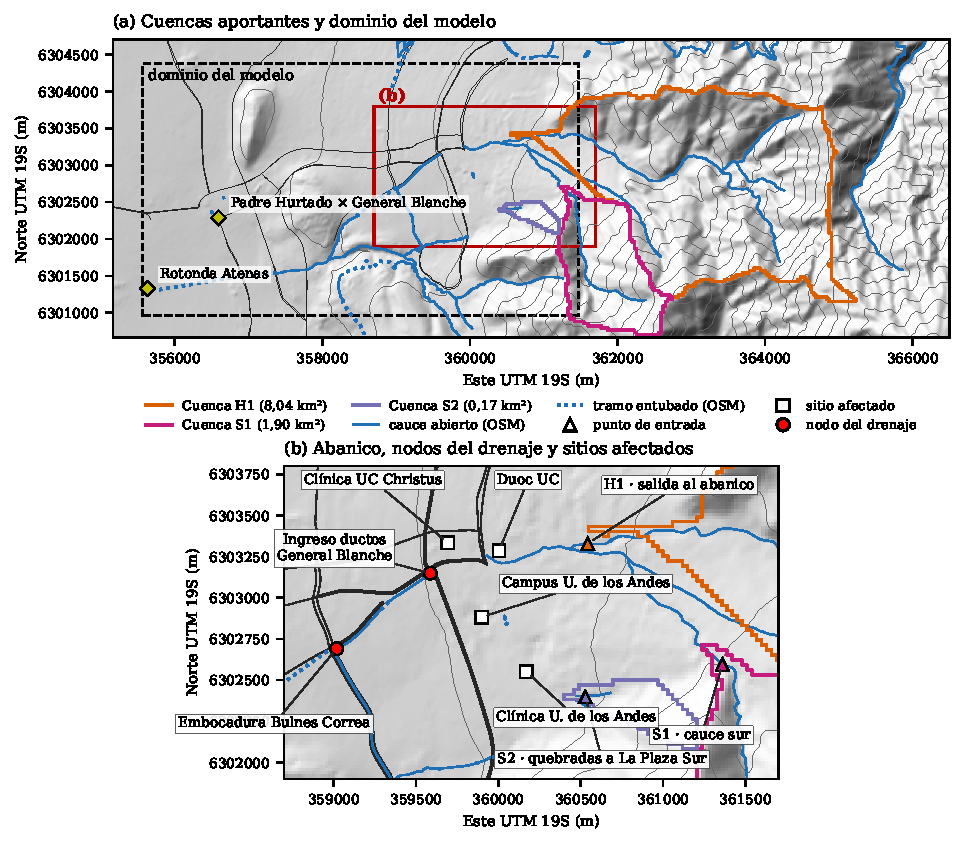
\includegraphics[width=\textwidth]{ubicacion}\caption{San Carlos de Apoquindo study area, Las Condes. (a) Contributing catchment boundaries calculated from the terrain (H1: main channel; S1: southern channel; S2: smaller ravines toward La Plaza Sur), open channels and piped reaches according to OpenStreetMap, model domain and downstream reference points. (b) Close-up of the alluvial fan: flow entry points, drainage nodes (entrance to the General Blanche conduits and Francisco Bulnes Correa culvert inlet) and sites with impacts reported by the sources collected in Section~\ref{sec:evidencia}. UTM coordinates, zone 19 south, WGS 84.}\label{fig:ubicacion}\end{figure}
\subsection{Evidence and Evidence Log}\label{sec:evidencia}
Every consultation of an external source was archived in an evidence log: UTC date and time, source, extracted data, page capture and SHA-256 hash. This records what information was available at the time of modeling and allows the prediction to be compared with subsequent observations. Observations were classified according to their physical nature, as recommended in the technical review (see the closing statement on the use of AI tools):
\begin{itemize}
\item \textbf{Reported presence:} streets along which the press reports that the flow ``descended'': Camino El Alba, General Blanche and Quebrada Honda \citep{latercera2026}; also Av.\ La Plaza, where T13 broadcast recordings of vehicles being swept away \citep{t13_2026vehiculos}.
\item \textbf{Municipal closures:} Mons.\ Álvaro del Portillo and Av.\ San Carlos de Apoquindo \citep{eldinamo2026}. These may reflect precautionary measures or cleanup.
\item \textbf{Municipal operational perimeter:} Camino El Alba to the north, La Plaza to the east, Quebrada Honda to the south and Padre Hurtado to the west \citep{latercera2026}. It may include dry areas.
\item \textbf{Reach:} to the Pueblito Los Dominicos area and Av.\ Padre Hurtado \citep{latercera2026}.
\item \textbf{Sites with reported flow presence:} the emergency department of Clínica UC Christus, with about \SI{1}{m} of mud \citep{cadena3_2026}; Clínica Universidad de los Andes, at its entrances and outside according to the clinic itself \citep{radiolasenal2026}; the Duoc UC campus \citep{biobio2026duoc}; and the Universidad de los Andes campus, whose community was stranded \citep{cooperativa2026}. Servicio Nacional de Prevención y Respuesta ante Desastres (Senapred) includes Av.\ La Plaza Sur among the affected areas \citep{eldinamo2026}.
\item \textbf{Low-reliability evidence, used only to formulate hypotheses:} an image circulated on social media marking several flow sources consistent with the mapped channels.
\end{itemize}
Rainfall data come from automatic station 330019 (Eulogio Sánchez, Tobalaba) of Dirección Meteorológica de Chile \citeyearpar{dmc2026}: \SI{34.8}{mm} on 8 October, \SI{13.8}{mm} between 15:00 and 21:00 local time, and, between 6 and 7 October, \SI{6}{h} reports totaling \SI{131.2}{mm}, with a maximum of \SI{49.2}{mm} in \SI{6}{h} (an earlier version of this text incorrectly attributed those \SI{49.2}{mm} to the two days). Press-search results recorded in the evidence log quoted figures of \SIrange{16}{20}{mm} in about one hour, with no station identified; these are unverified reported figures.

\paragraph{Hydrometeorological Information Obtained After Screening.} The mayor reported \SI{144}{mm} of accumulated rainfall in the area, \SI{20}{mm} of it on the day of the event, with saturated soil \citep{interferencia2026}. The analysis by Centro de Ciencia del Clima y la Resiliencia \citep{cr2_2026} records \SI{42.8}{mm} at Río Molina station on 8 October, \SI{31.6}{mm} between 15:00 and 19:00 and a maximum of \SI{10.9}{mm} in \SI{30}{min}, with the \SI{0}{\celsius} isotherm near \SI{2800}{m} according to the Cerro Tres Puntas observatory. The same analysis delineates the catchment between \SI{929}{m} and \SI{2355}{m} (about \SI{10.6}{km^2}) and estimates burn severity using the Sentinel-2 differenced normalized burn ratio (dNBR). The Open-Meteo historical hourly forecast \citep{openmeteo2023} places the isotherm between \SI{2700}{m} and \SI{2770}{m} between 14:00 and 17:00 on 8 October, and gives an accumulated total of about \SI{150}{mm} over the catchment between 2 and 8 October. This study’s interpretation of Sentinel-2 images \citep{drusch2012} from 21 September detected no snow in the catchment (calculated normalized difference snow index below 0.4 throughout the cloud-free portion; the white areas were interpreted as thin clouds), and this study’s analysis of those from 9 October estimates \SI{0.09}{km^2} of fresh snow, all above \SI{2000}{m}. The high Andes did have substantial snow cover: Valle Nevado reported about \SI{1.2}{m} of fresh snow on 6 and 7 October \citep{emol2026valle}, above \SI{3000}{m}.


\paragraph{Comparison with the CR2 Analysis.} Table~\ref{tab:cr2} compares the catchment and forcing data in this study with those in the CR2 analysis \citep{cr2_2026}, published after the hypotheses were formulated.
\begin{table}[htbp]\centering\small
\caption{Comparison of catchment and forcing data with the analysis by Centro de Ciencia del Clima y la Resiliencia (CR2) \citep{cr2_2026}. The difference in area and minimum elevation is due to the outlet location: CR2 places the catchment outlet farther downstream, in the linear park; this study places it where each channel enters the urban development.}\label{tab:cr2}
\begin{tabular}{p{0.24\textwidth}p{0.3\textwidth}p{0.36\textwidth}}\toprule
Variable & CR2 & This study (data and estimates)\\\midrule
Maximum catchment elevation & \SI{2355}{m} & \SI{2355}{m} (FABDEM and Copernicus GLO-30)\\
Minimum elevation & \SI{929}{m} & \SIrange{973}{1081}{m} (outlets H1, S1, S2)\\
Area & \SI{10.6}{km^2} & \SI{10.1}{km^2}\\
\SI{0}{\celsius} isotherm & $\sim\SI{2800}{m}$ (Cerro Tres Puntas) & \SIrange{2700}{2770}{m} between 14:00 and 17:00 (Open-Meteo)\\
Rainfall on 8 October & \SI{42.8}{mm} at Río Molina & same data\\
Fire & Sentinel-2 dNBR according to CR2 & dNBR (23-Dec-2025 and 6-Feb-2026): \SI{82}{\percent} with a burn signal and \SI{10}{\percent} moderate-high/high severity; used in the balance and in Gartner (Section~\ref{sec:res-incendio})\\
\bottomrule\end{tabular}
\end{table}

\paragraph{Later Assessments.} According to La Tercera, Senapred updated its assessment to 56 destroyed homes, 40 with major damage, 1,960 with minor damage, 384 people directly affected and more than 1,200 rescued \citep{latercera2026senapred}.

\subsection{Terrain, Buildings and Streets}\label{sec:terreno}
\emph{This section describes the terrain in the first model generation (1,103 buildings); the version with the full city (42,018 Overture Maps footprints, channels carved according to the official hydrographic network and about 852,000 triangles) is described in Section~\ref{sec:res-v4}.} The terrain without buildings or vegetation, i.e., the digital terrain model (DTM), is FABDEM V1-2 \citep{hawker2022,fabdem2023}, with a resolution of \SI{1}{\arcsecond} (about \SI{30}{m}), bilinearly resampled to a regular \SI{4}{m} grid in the UTM system, zone 19 south (WGS~84 datum). Resampling increases point density but does not improve the effective resolution of the elevation model. This limitation must be considered when interpreting the results. A total of \num{1107} building footprints from OpenStreetMap (OSM; \citealp{osm2026}) were incorporated as raised blocks. Each block's height is the mean of $\mathrm{DSM}-\mathrm{DTM}$, where the digital surface model (DSM) is Copernicus GLO-30 \citep{copernicus_glo30} and the DTM is FABDEM, when the footprint covers at least \SI{900}{m^2} and the difference exceeds \SI{2.5}{m}. Otherwise, the height is the OSM number of stories multiplied by \SI{3}{m}; without that information, \SI{6}{m} is assumed. The mean and 95th percentile of $\mathrm{DSM}-\mathrm{DTM}$ are reported for each block. Four OSM polygons tagged as buildings that correspond to facilities (sports complexes and a shopping center with mean $\mathrm{DSM}-\mathrm{DTM}$ below \SI{4}{m}) were excluded because, represented as solid blocks in the model, they would have artificially diverted the flow. Streets were lowered by \SI{0.15}{m}, the assumed curb height, with widths based on their category.

\subsection{Propagation Model}\label{sec:modelo}
ANUGA version 4.0.1 \citep{anuga} is used: finite volumes on an unstructured triangular mesh, with the DE1 scheme (second-order Runge--Kutta). For a homogeneous mixture of constant density, ANUGA solves the evolution of unit discharge $\mathbf q=h\mathbf u$ through the mass-conservation~\eqref{eq:masa} and momentum-conservation~\eqref{eq:movimiento} equations:
\begin{align}
\partial_t h+\nabla\cdot\mathbf q&=S_h,\label{eq:masa}\\
\partial_t\mathbf q+\nabla\cdot\left(\frac{\mathbf q\otimes\mathbf q}{h}+\tfrac12 gh^2\mathbf I\right)&=-gh\nabla z-\frac{\boldsymbol\tau_b}{\rho_m}+S_h\mathbf u_\mathrm{in},\label{eq:movimiento}
\end{align}
where $h$ is flow thickness (\si{m}); $\mathbf u$, depth-averaged velocity (\si{m.s^{-1}}); $\mathbf q=h\mathbf u$, discharge per unit width (\si{m^2.s^{-1}}); $z$, bed elevation (\si{m}); $g$, gravitational acceleration (\si{m.s^{-2}}); $S_h$, the rate of thickness input (\si{m.s^{-1}}); $\mathbf u_\mathrm{in}$, inflow velocity (\si{m.s^{-1}}); $\boldsymbol\tau_b$, basal shear stress (\si{Pa}); $\rho_m$, mixture density (\si{kg.m^{-3}}); and $\mathbf I$, the identity tensor. After dividing by the constant $\rho_m$, no density factor appears in the pressure or gravity terms. Basal resistance is $\boldsymbol\tau_b/\rho_m=ghS_f\,\mathbf u/U$, with $U=|\mathbf u|$ and friction slope $S_f$ given by
\begin{equation}
S_f=\frac{\tau_y}{\rho_m g h}+\frac{K\eta U}{8\rho_m g h^2}+\frac{n_\mathrm{td}^2U^2}{h^{4/3}},\label{eq:friccion}
\end{equation}
where $\tau_y$ is yield stress (\si{Pa}); $\eta$, the dynamic viscosity of the mixture (\si{Pa.s}); $K$, the dimensionless laminar resistance parameter; and $n_\mathrm{td}$, the equivalent Manning coefficient for turbulence and dispersion (\si{s.m^{-1/3}}). Yield stress and viscosity are obtained from the rheological relationships
\begin{equation}
\tau_y=0.1\,\alpha_2e^{\beta_2\Cvf},\qquad \eta=0.1\,\alpha_1e^{\beta_1\Cvf},\label{eq:reologia}
\end{equation}
where $\Cvf$ is the volumetric concentration of the fine matrix; in contrast, density $\rho_m$ uses the total concentration $\Cvt$ (Section~\ref{sec:marco}). The sweep simulations adopt $\Cvt=\Cvf$. The coefficients $(\alpha_1,\beta_1,\alpha_2,\beta_2)$ come from Table~13 of \citet{flo2d2021}, where $\alpha_1$ is expressed in poise and $\alpha_2$ in \si{dyn.cm^{-2}}; $\beta_1$ and $\beta_2$ are dimensionless. The factor 0.1 in~\eqref{eq:reologia} converts both quantities to SI units, so that $\tau_y$ is in \si{Pa} and $\eta$ in \si{Pa.s}. The Glenwood~2 sample appears in three variants in different versions of the documentation and was treated as a sensitivity test. $K$ and $n_\mathrm{td}$ vary by surface: on paved streets $K=100$ and $n_\mathrm{td}=0.025$; elsewhere, $K=400$ and $n_\mathrm{td}=0.050$.

Resistance~\eqref{eq:friccion} is applied as a fractional step and solved implicitly in each cell. With $a=\tau_y/(\rho_m h)$, $b=K\eta/(8\rho_m h^2)$, $c=gn_\mathrm{td}^2/h^{4/3}$ and $r=(U^*-\Delta t\,a)_+$, the result is
\begin{equation}
U^{n+1}=\frac{2r}{1+b\Delta t+\sqrt{(1+b\Delta t)^2+4c\Delta t\,r}},\label{eq:resistencia}
\end{equation}
where the asterisk indicates the state before the resistance step; the superscript $n+1$, the state after that step; $\Delta t$ is the time step and $(x)_+=\max(x,0)$. Solution~\eqref{eq:resistencia} satisfies $0\le U^{n+1}\le U^*$, preserves direction, dissipates energy and does not modify $h$. If $|\mathbf q^*|\le\Delta t\,\tau_y/\rho_m$, the cell stops and may reactivate in subsequent steps. ANUGA's own Manning friction is set to zero to avoid duplicating resistance.

The mixture enters through a triangular hydrograph with peak discharge $Q_p$, mixture volume $V_m$ and time to peak of \SI{600}{s}, with base $T_B=2V_m/Q_p$. In a circle of radius \SI{14}{m}, each source adds the thickness increment $\Delta h$ corresponding to the volume supplied by the hydrograph during the step, together with its momentum: $h^+=h^-+\Delta h$ and $\mathbf q^+=\mathbf q^-+\Delta h\,\mathbf u_\mathrm{in}$, where superscripts $-$ and $+$ indicate the states before and after the input, and $\mathbf u_\mathrm{in}$ is oriented along the channel axis. When $Q=0$, there is no forcing. In H3, each source receives the fraction of the hydrograph corresponding to its catchment area. The first-generation mesh has about \num{4.3e5} triangles: \SI{40}{m^2} in the corridor between the channels and Padre Hurtado (equivalent side length of about \SI{10}{m}) and \SI{600}{m^2} outside it. Gravitational acceleration is $g=\SI{9.8}{m.s^{-2}}$ throughout the model. In the first generation, simulations last $T_B+\SI{1200}{s}$, and the volume balance is recorded in each. The city, measured-rainfall and fine-campus-mesh variants are described in Sections~\ref{sec:res-v4} and~\ref{sec:res-posterior}.

\begin{table}[htbp]\centering\small
\caption{Physical and numerical parameters applied in the simulations. Rheological coefficients are from the O'Brien and Julien sample table compiled in the FLO-2D manual \citep{flo2d2021}; $\tau_y=0.1\,\alpha_2e^{\beta_2C_v}$ in Pa and $\eta=0.1\,\alpha_1e^{\beta_1C_v}$ in Pa\,s.}\label{tab:parametros}
\begin{adjustbox}{max width=\textwidth}\begin{tabular}{lrrrrrrr}\toprule
Sample & $\alpha_1$ & $\beta_1$ & $\alpha_2$ & $\beta_2$ & \multicolumn{3}{c}{$\tau_y$ (Pa) / $\eta$ (Pa\,s) with $C_v=$}\\\cmidrule(l){6-8}
 & & & & & 0.35 & 0.40 & 0.45\\\midrule
Glenwood 1 & 0.0028 & 23.00 & 0.0345 & 20.10 & 3.9 / 0.89 & 10.7 / 2.80 & 29.2 / 8.85\\
Glenwood 2a & 0.0648 & 6.20 & 0.0765 & 16.90 & 2.8 / 0.06 & 6.6 / 0.08 & 15.4 / 0.11\\
Glenwood 2b & 0.6480 & 6.20 & 0.0765 & 16.90 & 2.8 / 0.57 & 6.6 / 0.77 & 15.4 / 1.06\\
Glenwood 2c & 0.6480 & 8.20 & 0.0765 & 16.90 & 2.8 / 1.14 & 6.6 / 1.72 & 15.4 / 2.59\\
Aspen 1 & 0.0360 & 22.10 & 0.1810 & 25.70 & 145.9 / 8.23 & 527.5 / 24.86 & 1,906.8 / 75.05\\
Aspen 2 & 0.0538 & 14.50 & 2.7200 & 10.40 & 10.4 / 0.86 & 17.4 / 1.78 & 29.3 / 3.67\\
\midrule
\multicolumn{8}{l}{\textbf{Mixture and constants}}\\
\multicolumn{5}{l}{Water density $\rho_w$ / solids density $\rho_s$} & \multicolumn{3}{r}{\SI{1000}{kg/m^3} / \SI{2650}{kg/m^3}}\\
\multicolumn{5}{l}{Mixture density $\rho_m=\rho_w+C_v(\rho_s-\rho_w)$, $C_v=0.35/0.40/0.45$} & \multicolumn{3}{r}{1,578 / 1,660 / 1,742 kg/m$^3$}\\
\multicolumn{5}{l}{Gravity $g$} & \multicolumn{3}{r}{\SI{9.8}{m/s^2}}\\
\multicolumn{5}{l}{Laminar resistance $K$ (streets / elsewhere)} & \multicolumn{3}{r}{100 / 400}\\
\multicolumn{5}{l}{Turbulent-dispersive Manning $n_{td}$ (streets / elsewhere)} & \multicolumn{3}{r}{0.025 / 0.050 s\,m$^{-1/3}$}\\
\multicolumn{8}{l}{\textbf{Input, mesh and computation}}\\
\multicolumn{5}{l}{Mixture volume $V$ / peak discharge $Q_p$ / time to peak $t_p$} & \multicolumn{3}{r}{80--300 thousand m$^3$ / 100--250 m$^3$/s / 600 s}\\
\multicolumn{5}{l}{Inflow velocity / radius of each source} & \multicolumn{3}{r}{2 m/s / 14 m}\\
\multicolumn{5}{l}{Maximum triangle area (corridor / elsewhere); triangles, first model generation} & \multicolumn{3}{r}{40 / 600 m$^2$; $\approx$430,000}\\
\multicolumn{5}{l}{Terrain grid; street lowering; assumed building height} & \multicolumn{3}{r}{4 m; 0.15 m; 6 m}\\
\multicolumn{5}{l}{Courant number (screening / rainfall / final)} & \multicolumn{3}{r}{1 / 0.5 / $\le$0.25}\\
\multicolumn{5}{l}{Wetting threshold for evaluation $h^*$} & \multicolumn{3}{r}{5 cm (sensitivity 2 and 10 cm)}\\
\bottomrule\end{tabular}\end{adjustbox}\end{table}

\begin{figure}[htbp]\centering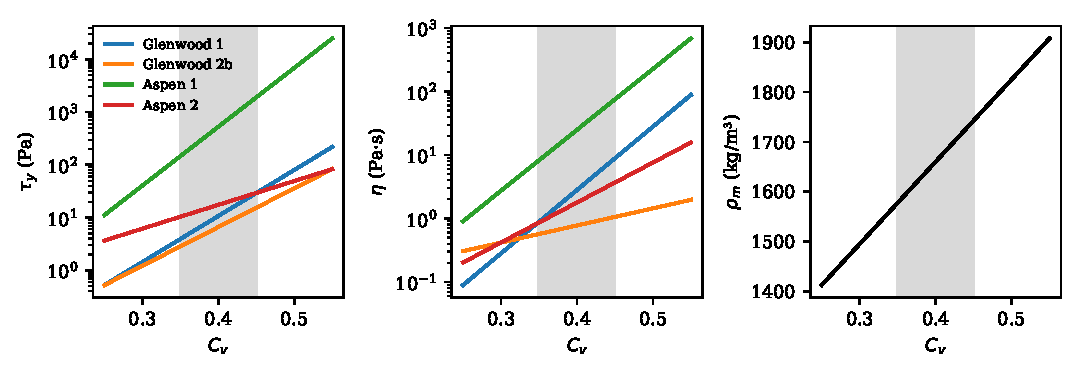
\includegraphics[width=\textwidth]{reologia}\caption{Calculated mixture properties as a function of volumetric solids concentration $C_v$ for the samples tested: yield stress $\tau_y$, viscosity $\eta$ and density $\rho_m$. The gray band indicates the initial range (0.35--0.45); subsequent tests extend the concentrations (Section~\ref{sec:res-posterior}).}\label{fig:reologia}\end{figure}

\subsection{Numerical Verification}\label{sec:verif}
\paragraph{Stopping.} On a plane with slope $S_0=0.05$, with $\tau_y=\SI{100}{Pa}$ and $\rho_m=\SI{1700}{kg.m^{-3}}$, depth-integrated Bingham-fluid theory predicts a static thickness $h_c=\tau_y/(\rho_m gS_0)=\SI{0.1200}{m}$. A block of mixture is released and the simulated deposit thickness is compared with the theoretical static thickness; it is also verified that momentum falls to zero.

\paragraph{Restart.} Mixture is added upstream of the stopped deposit, and it is verified that the deposit restarts, stops again and conserves volume.

\paragraph{Temporal Convergence.} The stopping test is repeated with Courant--Friedrichs--Lewy (CFL) numbers of 1, 0.5, 0.25, 0.1 and 0.05 using the DE1 scheme, and with the DE0 scheme for comparison; the final front reach is compared and the order of convergence relative to the extrapolated limit is estimated.

\paragraph{Volume Balance.} In each simulation, the cumulative volume supplied by the hydrograph is compared with the volume present in the mesh.

The results of these tests are presented in Section~\ref{sec:res-verif}.

\subsection{Independent Prior Volume Estimate}\label{sec:volumen}
Catchments were delineated using flow directions calculated with the eight-direction (D8) method on FABDEM reprojected to the UTM system, zone 19 south (WGS~84 datum), with \SI{30}{m} cells. A preliminary delineation in geographic coordinates underestimated the area. The outlet of each catchment is the cell with the greatest flow accumulation within \SI{120}{m} of the point where the mapped channel enters the urban development. The resulting areas are H1 with \SI{8.04}{km^2} and relief of \SI{1376}{m}, S1 with \SI{1.90}{km^2} and S2 with \SI{0.17}{km^2}: a total contributing area of \SI{10.1}{km^2}.

Two independent estimates were used, without combining them into a single distribution:
\begin{itemize}
\item \textbf{Rainfall--runoff balance with water and solids distinguished:} $V_w=f_wPAC$ and $V_m=V_w/(1-\Cvt)$, where $V_w$ is the water volume incorporated into the pulse; $P$, accumulated precipitation; $A$, catchment area; $C$, the runoff coefficient; $f_w$, the fraction of runoff incorporated into the pulse; and $V_m$, mixture volume. The ranges are: event-pulse precipitation $P$ between \SI{12}{\milli\metre} and \SI{35}{\milli\metre}, $C\in[0.3;0.8]$, $f_w\in[0.5;1]$ and $\Cvt\in[0.30;0.50]$.
\item \textbf{Empirical model for burned catchments} \citep{gartner2014}, applied by subcatchment and including its residual error $\varepsilon\sim N(0;1.04^2)$. This model predicts deposit volume $V_\mathrm{dep}$, which is converted to mixture volume using $V_m=(1-\phi)V_\mathrm{dep}/\Cvt$, where $\phi$ is deposit porosity. Its applicability outside southern California is a hypothesis.
\end{itemize}
The distributions are summarized by the median and the 5th and 95th percentiles, and the corresponding peak discharge is estimated using the relationship of \citet{mizuyama1992}. Calibration spans volumes from \SI{80000}{\metre\cubed} to \SI{300000}{\metre\cubed}. Initial results are presented in Section~\ref{sec:res-volumen}; the update with severity estimated by dNBR is presented in Section~\ref{sec:res-incendio}.

\begin{figure}[htbp]\centering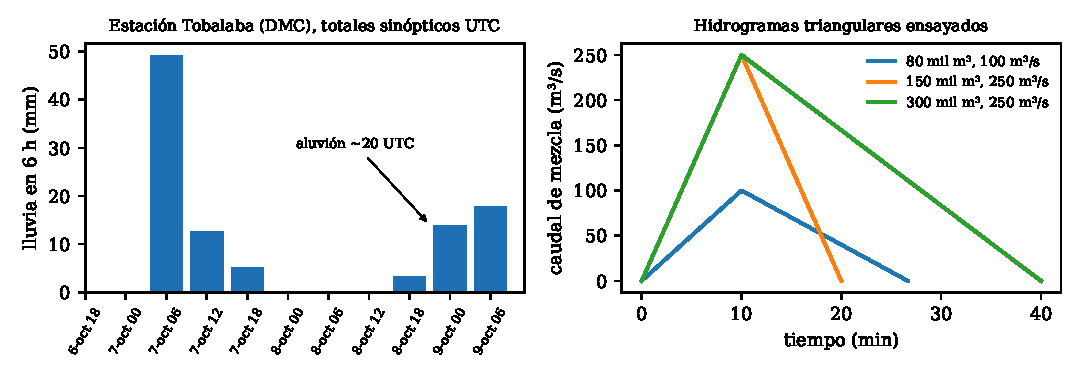
\includegraphics[width=\textwidth]{forzamiento}\caption{Observed and assumed model forcing. Left: rainfall accumulated over \SI{6}{h} intervals at the Tobalaba station of Dirección Meteorológica de Chile \citep{dmc2026} between 6 and 9 October 2026 (UTC times; the press reports cited in the account place the debris flow at about 20 UTC on 8 October). Right: triangular mixture hydrographs tested.}\label{fig:forzamiento}\end{figure}

\paragraph{Saturated-Soil Scenario.} With the hydrometeorological information obtained after screening (Section~\ref{sec:evidencia}), a third estimate was added, also without combining it with the previous ones. The relationship between the reported isotherm and the maximum catchment elevation (\SI{2355}{m}, the same as reported by CR2; an earlier version of the text mistakenly stated \SI{2775}{m}, a figure not used in any calculation: D8 delineation and hypsometry were always based on the elevation model) supports the assumption of liquid precipitation over the entire contributing area, and the soil saturation reported by the authority is adopted as an assumption of the calculation scenario. The ranges used are $P\in[20;40]$~\si{mm}, $C\in[0.6;0.9]$ and $f_w\in[0.6;1]$. The snowmelt contribution is bounded above by \SI{50}{mm} water equivalent over the \SI{0.31}{km^2} of the catchment above \SI{2000}{m}.

\subsection{Inverse Calibration and Uncertainty}\label{sec:calib}
Calibration follows the approach of retaining simulations that meet the acceptance criteria \citep{beven1992}. The criteria were specified before examining the results:
\begin{enumerate}
\item fraction $R$ of points on streets with reported flow presence at which $h_\mathrm{max}>h^*$, with $R\ge0.6$;
\item fraction $R_\mathrm{sit}$ of the four sites with reported flow presence that the flow reaches within \SI{40}{m}, with $R_\mathrm{sit}\ge3/4$;
\item arrival within \SI{200}{m} of the intersection of General Blanche and Padre Hurtado;
\item fraction $F_\mathrm{per}$ of the simulated affected area falling within the municipal perimeter expanded by \SI{100}{m}, with $F_\mathrm{per}\ge0.5$. Since 11 October, when the official affected area was published \citep{bbnn2026visor}, $F_\mathrm{per}$ has been calculated using that polygon and only for simulated mud in urban areas (within \SI{40}{m} of a building), to avoid counting hills wetted by rainfall.
\end{enumerate}
The threshold is $h^*=\SI{5}{cm}$, with sensitivity tests for \SI{2}{cm} and \SI{10}{cm}. Each acceptable simulation receives an informal weight $L=R\,R_\mathrm{sit}\,F_\mathrm{per}$. Streets closed by the municipality are used only as context, because a closure may be precautionary. The Jaccard index relative to the perimeter is reported descriptively, since the perimeter is operational rather than a mapped footprint.

The sweep covers hypotheses H1, H2 and H3; mixture volumes of \SI{80000}{\metre\cubed}, \SI{150000}{\metre\cubed} and \SI{300000}{\metre\cubed}; peak discharges of \SI{100}{\metre\cubed\per\second} and \SI{250}{\metre\cubed\per\second}; and three rheological samples (Glenwood~1, Glenwood~2b and Aspen~2). Screening used CFL~1. Checks with a fine time step (z01, z02, z26, z29 and z32) and the test with a fine mesh on campus (m36) were completed, as described in Sections~\ref{sec:res-verif} and~\ref{sec:res-posterior}.

\subsection{Ensemble Synthesis and Indicators by Street and Building}\label{sec:sintesis}
\paragraph{Three Levels of Evaluation.} Three levels are distinguished: (i) the \emph{original acceptance criteria}, specified before simulation with a threshold for each (Section~\ref{sec:calib}); with the previous terrain, no simulation met all of them; the candidate for the held-out test (z02) meets three of four (not meeting the perimeter criterion), while the subsequent porous-house fit (z26) and the integrated hypothesis with assumed rainfall (z32) meet all four; (ii) the \emph{exploratory compatibility index} (ECI), defined later, which summarizes the same four criteria on a continuous scale to compare hypotheses; and (iii) \emph{independent validation} of subsequent fits, untested at closure, which requires data not used to formulate the hypotheses, such as post-event satellite images, official deposit surveys or high-water marks.

\paragraph{Exploratory Compatibility Index.} To compare hypotheses, each simulation is summarized by an \emph{exploratory compatibility index} (ECI) of agreement with observations, on a scale from 0 to 100: the average of four components, each between 0 and 1, derived from the original criteria specified before simulation (Section~\ref{sec:calib}); the index was defined later and the perimeter reference was updated with the official polygon. These components are the fraction of points on streets with mud reported by the sources that the model wets ($R$); the fraction of the four facilities with reported impacts that are reached ($R_\mathrm{sit}$); reach, equal to 1 if the mud arrives within \SI{200}{m} of Padre Hurtado and decreasing linearly to 0 at \SI{1200}{m}; and $F_\mathrm{per}$. The ECI is neither a probability nor a measure of predictive accuracy: it summarizes how well a simulation reproduces a set of qualitative observations, and differences of two or three points should not be interpreted as conclusive evidence that one hypothesis is superior to another. Depths, velocities and pressures by street and building are extracted as the maximum within a radius of \SI{40}{m} of each point of interest.


\section{Model Inputs and Operation: A Guide to Application in Other Catchments}\label{sec:transferencia}
This section describes the method in general terms, without reference to specific products or programs, so that it can be applied to other catchments with the data available in each case. It explains what each input represents, the recommended minimum quality, how it enters the calculation and how its uncertainty affects the result.

\subsection*{How the Model Works}
At every instant and in every cell of a mesh covering the city, the model solves for how much mud is present (thickness), in which direction it moves and at what velocity. It does so using three principles:
\begin{enumerate}
\item \textbf{Conservation of mass:} mud entering a cell without leaving accumulates as thickness. Mud is neither created nor lost; the balance is verified in every simulation.
\item \textbf{Conservation of momentum:} mud accelerates downslope under gravity, according to the slope of the free surface and not just that of the ground, and is slowed by the material's own resistance and friction with the surface. This allows it to flow over a curb if it arrives with velocity, go around a building or pond behind an obstacle.
\item \textbf{Material behavior:} unlike water, a dense mixture of water and sediment has a \emph{yield threshold}: if the gravitational driving stress on a layer does not exceed it, the layer stops. This is why mud leaves deposits of a certain thickness instead of draining to the lowest elevation. Above that threshold, the mixture behaves as a highly viscous and turbulent fluid.
\end{enumerate}
The simulation advances in short time steps, of fractions of a second, limited by flow velocity and cell size. Each step first calculates transport and gravity, then material resistance, which can stop a cell or allow it to reactivate if more mud arrives from upstream. During the simulation, maximum thickness, maximum velocity, dynamic loading on obstacles and front arrival time are recorded for each cell.

\subsection*{Input Data}
\begin{table}[htbp]\centering\small
\caption{Input data for applying the model to other catchments: meaning, recommended quality and effect of uncertainty on calculated results.}\label{tab:transferencia}
\begin{tabular}{p{0.17\textwidth}p{0.25\textwidth}p{0.22\textwidth}p{0.245\textwidth}}\toprule
Data & What they represent and how they are used & Recommended quality & Effect of uncertainty\\\midrule
Bare-earth topography & Ground elevations without buildings or trees; defines slopes and flow directions. & Preferably \SIrange{1}{5}{m} resolution; \SI{30}{m} only reproduces the general direction. & The most influential input: a channel or street unresolved by the terrain changes the flow path.\\
Building footprints and heights & Obstacles that flow goes around; raised above the terrain. & Complete footprints; height from surveys or number of stories. & Divert flow locally; little influence on the general path if the footprints adequately represent building geometry.\\
Streets and curbs & Preferential corridors; lowered a few centimeters relative to sidewalks. & Centerline and width of each street; curb elevation if available. & Determine which streets act as channels.\\
Open channels and piped reaches & Where the ravine flows on the surface and where underground; transition points are potential overflow locations. & Alignment, cross section and capacity of each reach. & If an open channel is missing, the model substitutes the general slope; if a conduit is missing, its overflow cannot be evaluated.\\
Contributing catchment & Area and relief draining to each entry point into the city; derived from the terrain. & Terrain of the upper catchment; \SI{30}{m} is usually sufficient. & Scales expected volume in proportion to area.\\
Rainfall & Amount and intensity of the episode and preceding days (soil moisture). & Nearby station with hourly or subhourly records; ideally in the upper catchment. & Together with the catchment, constrains volume; short-duration intensity controls peak discharge.\\
Catchment condition & Burned area, vegetation cover, soil. & Burn-severity mapping. & Conditions the assumed runoff and sediment-load coefficients.\\
Volume and hydrograph & How much mixture enters, at what maximum discharge and over what time. & Estimated from rainfall and catchment, empirical relationships or deposits measured after the event. & Control reach and depths; constrained through calibration.\\
Material properties & Mixture density, yield threshold and viscosity, as a function of solids concentration. & Tests on deposit samples; otherwise, ranges from the literature. & Control when and where flow stops.\\
Event observations & Affected streets and buildings, reach, depths, times. & Georeferenced points with source and time; high-water marks. & Not model inputs: allow hypotheses to be rejected and calibration to be performed.\\
\bottomrule\end{tabular}\end{table}

\subsection*{Procedure for Another Catchment}
\begin{enumerate}
\item \textbf{Delineate the exposed urban area} and the points where channels enter the city or change from open to piped. These points are possible flow inputs.
\item \textbf{Construct the computational surface:} bare-earth topography, raised buildings, lowered streets and, if possible, open channels with their actual cross sections.
\item \textbf{Estimate a volume range} using at least two independent approaches (rainfall times catchment area times runoff coefficient, and empirical relationships for similar catchments), without combining them into a single figure.
\item \textbf{Formulate input hypotheses} (the points where flow emerges at the surface and in what proportions) and specify, \emph{before} simulation, the criteria for judging each against the observations.
\item \textbf{Simulate every combination} of hypothesis, volume, discharge and material; verify mass balance and numerical stability in each simulation.
\item \textbf{Compare with the observations}, retain compatible combinations and report the ensemble as a range of scenarios rather than a single answer.
\item \textbf{Repeat compatible simulations at higher temporal and spatial resolution} to estimate the numerical error in reaches and times.
\end{enumerate}

\subsection*{What Most Improves the Result}
In this case study, uncertainties ranked by influence were: terrain (resolution and representation of channels and streets), material properties, volume and hydrograph shape, and building heights. A high-resolution survey of the urban area and channel, and deposit samples, are the two improvements with the greatest benefit. For prevention purposes, without an event to calibrate against, the method is applied in the same way, but with volume and material scenarios chosen according to the catchment and with impact envelopes reported instead of a single flow path.


\section{Results}\label{sec:resultados}
\emph{Results at closure (13 October 2026): 84 completed simulations, 19 screening runs with the previous terrain, 41 with the full city, 5 concentration quadrature runs and 19 campus micro-simulations. Sections~\ref{sec:res-v4} to~\ref{sec:res-campus} use the terrain with the full city; Section~\ref{sec:res-calib} retains the initial screening with the previous terrain as a record of the process.}

\subsection{Simulations with the Full City}\label{sec:res-v4}
The terrain version used for the urban results incorporates all 42,018 Overture Maps building footprints over FABDEM at \SI{4}{m}, extends the domain to Paul Harris, Hospital Dipreca and the Atenas roundabout, and carves three channels that the \SI{30}{m} elevation model does not resolve: the linear park to the Francisco Bulnes Correa culvert inlet, Quebrada Honda downstream of the inlet according to the official hydrographic network, and the southern branch to the upper part of Av.\ Monseñor Álvaro del Portillo. The mesh has about 852,000 triangles. Table~\ref{tab:v4} summarizes the simulations; Appendix~\ref{sec:anexo} contains the catalog of screening, city and quadrature runs and a fact sheet with a figure for each key simulation.

\begin{table}[htbp]\centering\small
\caption{Simulations with the full city (42,018 buildings). Culvert capacities are assumed parameters of hypothetical scenarios; they do not describe the real structure. Streets: fraction of points on streets with mud reported by the sources that the model wets ($h>\SI{5}{cm}$); Sites: fraction of the four facilities with reported impacts that are reached by the simulated flow; dPH: minimum simulated mud distance to the intersection of General Blanche and Padre Hurtado; Perim.: fraction of simulated mud in urban areas falling within the official affected area (IDE Chile); QH: fraction of Quebrada Honda with simulated mud; UCC: maximum calculated thickness next to Clínica UC Christus (Cadena 3 reported about \SI{1}{m} in the emergency department); ECI: exploratory compatibility index, average of the four criteria (streets, sites, reach and perimeter) on a scale from 0 to 100; it is not predictive accuracy. Mud: G2b, Glenwood~2b ($C_v=0.40$); G1, Glenwood~1 ($C_v=0.45$); A2, Aspen~2.}\label{tab:v4}
{\setlength{\tabcolsep}{3.5pt}\begin{adjustbox}{max width=\textwidth}\begin{tabular}{llrlrrrrrrr}\toprule
Run & Scenario & $V$ (thousand m$^3$) & Mud & Streets & Sites & dPH (m) & Perim. & QH & UCC (m) & ECI\\
\midrule
z02 & channel + southern branches; rainfall 35 mm/h, time step 4× finer & 300 & G2b & 0.77 & 0.75 & 15 & 0.34 & 0.68 & 1.13 & 72\\
v02 & channel + southern branches; rainfall 35 mm/h on hillside & 300 & G2b & 0.77 & 0.75 & 15 & 0.34 & 0.68 & 1.13 & 72\\
v19 & channel + southern branches; rainfall 35 mm/h + official southern branch to Álvaro del Portillo (terrain v6) & 300 & G2b & 0.77 & 0.75 & 15 & 0.34 & 0.68 & 1.11 & 71\\
v14 & channel + southern branches; rainfall 35 mm/h + Álvaro del Portillo ravine & 300 & G2b & 0.77 & 0.75 & 15 & 0.34 & 0.68 & 1.15 & 71\\
v01 & main channel & 300 & G2b & 0.77 & 0.50 & 96 & 0.46 & 0.68 & 1.16 & 68\\
z01 & main channel; numerical check (time step 4× finer) & 300 & G2b & 0.77 & 0.50 & 96 & 0.46 & 0.68 & 1.16 & 68\\
v15 & main channel; Quebrada Honda carved downstream (terrain v5) & 300 & G2b & 0.77 & 0.50 & 96 & 0.45 & 0.68 & 1.18 & 68\\
v03 & main channel; culvert with assumed capacity of 30 m$^3$/s & 300 & G2b & 0.77 & 0.50 & 96 & 0.50 & 0.64 & 1.16 & 69\\
v17 & main channel; culvert with assumed capacity of 30 m$^3$/s, capture 25 m, Quebrada Honda carved & 300 & G2b & 0.76 & 0.50 & 96 & 0.50 & 0.62 & 1.18 & 69\\
v05 & main channel; culvert with assumed capacity of 100 m$^3$/s & 300 & G2b & 0.74 & 0.50 & 96 & 0.53 & 0.44 & 1.16 & 69\\
v10 & main channel; culvert with assumed capacity of 100 m$^3$/s, capture 25 m & 300 & G2b & 0.69 & 0.50 & 96 & 0.52 & 0.00 & 1.16 & 68\\
v18 & main channel; culvert with assumed capacity of 100 m$^3$/s, capture 25 m, Quebrada Honda carved & 300 & G2b & 0.69 & 0.50 & 96 & 0.52 & 0.00 & 1.18 & 68\\
v07 & main channel & 150 & G2b & 0.72 & 0.50 & 348 & 0.62 & 0.68 & 1.09 & 67\\
v08 & main channel & 300 & G1 & 0.74 & 0.50 & 396 & 0.63 & 0.69 & 1.16 & 67\\
v09 & main channel & 300 & A2 & 0.77 & 0.50 & 151 & 0.52 & 0.68 & 1.14 & 70\\
v21 & channel + southern branches; official southern branch (terrain v6), without rainfall & 300 & G2b & 0.77 & 0.50 & 131 & 0.45 & 0.68 & 1.11 & 68\\
\bottomrule\end{tabular}\end{adjustbox}}
\end{table}


Four results stand out:
\begin{enumerate}
\item \textbf{The represented city channels the mud in the model.} With all buildings, the calculated thickness around Clínica UC Christus increases from \SI{0.3}{m} to \SIrange{1.1}{1.2}{m}, comparable in magnitude to the meter reported by Cadena 3 in its emergency department \citep{cadena3_2026} (a maximum near the facility does not necessarily represent its interior), and reaches \SI{1.9}{m} next to Duoc UC. Mud runs deeper along the streets and covers less area: about \SI{54}{ha} within the official affected area, compared with \SI{93}{ha} with the previous terrain.
\item \textbf{Volume.} In the model, with \SI{150000}{m^3}, the front stops \SI{348}{m} from Padre Hurtado; with \SI{300000}{m^3}, it comes within \SI{100}{m}. That volume agrees with the independent estimate assuming saturated soil (Section~\ref{sec:res-volumen}).
\item \textbf{Hypothesis selected for the held-out test.} The main channel plus the southern branches and rainfall of \SI{35}{mm/h} on the hillside (z02, v02) obtains an ECI of 72/100 (streets 0.77; facilities 0.75; reach 1.00; official affected area 0.34): it reproduces flow presence at \SI{77}{\percent} of control points on the streets considered, three of the four facilities---including Clínica Universidad de los Andes, with \SI{0.14}{m}---and the reach, but only one third of its urban mud falls within the official affected area. Without the assumed rainfall on the hillside (v21), the model does not reach Clínica Universidad de los Andes and the ECI falls to 68/100.
\item \textbf{Robustness.} z02 repeats v02 with a time step four times smaller and gives the same indicators; z01 does the same for the main channel alone. The very fluid mud mixture (Aspen~2) obtains 70/100; the thick mixture (Glenwood~1) stops \SI{396}{m} from Padre Hurtado. The ECI of v20 with the normal time step (78/100) depends on \SI{10}{cm} at a single point on the campus and is not reproduced with a fine time step (v19), so it is not considered.
\end{enumerate}

\subsection{Assumed Francisco Bulnes Correa Culvert Capacity: Hypothetical Scenarios}\label{sec:res-colector}
This section is an analysis of hypothetical scenarios. Public information on the actual capacity, cross section and condition of the culvert was unavailable; the following values do not evaluate the structure or constitute an official conclusion, and require validation with design and inspection information. \emph{Calculated result:} with the full city and the adopted volume hypothesis, the mixture discharge reaching the culvert inlet peaks at about \SI{65}{m^3/s}, four times that with the previous terrain. \emph{Hypothetical scenarios:} if the model sink captures the entire channel cross section (capture radius of \SIrange{25}{40}{m}), with an assumed capacity of \SI{100}{m^3/s} or \SI{200}{m^3/s} it removes about \SI{93000}{m^3} with a peak of \SIrange{62}{66}{m^3/s}, and Quebrada Honda remains dry (v10, v11, v18). With an assumed capacity of \SI{30}{m^3/s}, the sink reaches that limit, removes \SI{67600}{m^3}, and Quebrada Honda is wetted at \SI{62}{\percent} of its points (v17). In these scenarios, the calculated range of assumed capacity that leaves no surface flow downstream of the sink lies between \SI{30}{m^3/s} and about \SI{65}{m^3/s}; that interval depends on the assumed volume, hydrograph and rheology. \emph{Why this changed relative to the first model generation.} With 1,103 buildings, mud spread across the surface and \SI{12800}{m^3} reached the culvert inlet with a peak of \SI{16.5}{m^3/s}, which the model sink with an assumed capacity of \SI{30}{m^3/s} removes. In the model with the 42,018 footprints, streets concentrate the flow, increase velocity and deliver about \SI{93000}{m^3} to the inlet with a peak near \SI{65}{m^3/s}. Both results are calculated and depend on the urban representation; the version with the full city is the current one. A capture radius of \SI{12}{m} allowed flow to pass beside the sink and produced mud at \SI{44}{\percent} of Quebrada Honda even with \SI{100}{m^3/s}; this was a representation artifact, corrected by capturing the entire cross section. Official hydrographic mapping represents channel continuity from the culvert inlet along Quebrada Honda toward Hospital Dipreca; in the simulations, flow not removed by the sink representing the culvert continues along that alignment.

\subsection{Comparison with the Official Affected Area}\label{sec:res-oficial}
The emergency viewer of Ministerio de Bienes Nacionales, developed by IDE Chile, publishes the affected area (\SI{288.5}{ha}), 2,266 properties and 368 affected street segments \citep{bbnn2026visor}. The area is the strip between two corridors: Camino El Alba and General Blanche to the north, and Quebrada Honda to the south, with an extension along Camino El Alba west of Padre Hurtado (Figure~\ref{fig:ide}). Simulated mud runs along these two edges, but leaves the interior of the strip dry and extends beyond it in three sectors: the hills and ravines wetted by rainfall on the hillside, the street network west of Padre Hurtado (\SIrange{8}{20}{ha}), and Quebrada Honda downstream toward Dipreca (\SIrange{14}{26}{ha}), with thicknesses of \SIrange{0.3}{0.4}{m}. Since the published properties represent the full set within the perimeter rather than properties with verified mud (\SI{91}{\percent} are inside the area), the fraction of properties touched by simulated mud (717 of 2,266, \SI{32}{\percent} in z02) serves to compare simulations, not as an accuracy rate. With this polygon, the perimeter criterion decreases and the ECI of z02 changes from 74/100 (press perimeter) to 72/100.

\begin{figure}[htbp]\centering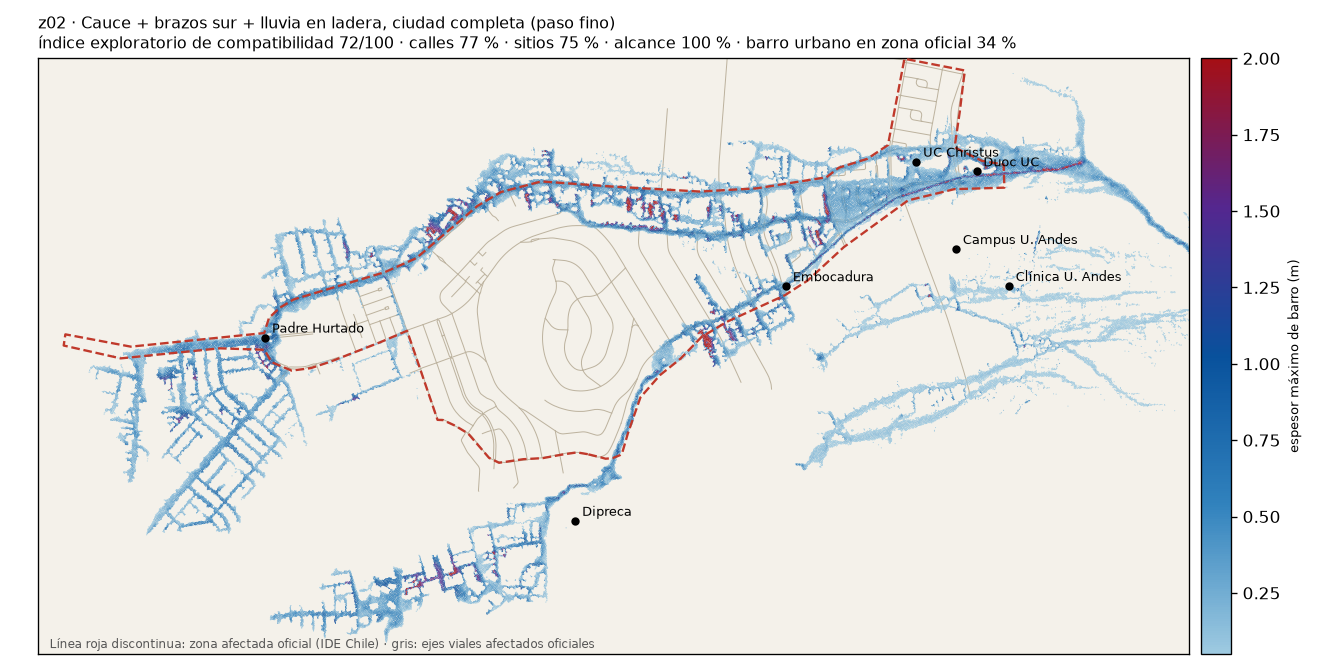
\includegraphics[width=\textwidth]{anexo/z02}\caption{Simulation z02 (main channel, southern branches and assumed hillside rainfall, fine time step) over the official affected area from IDE Chile (dashed red line) and affected street centerlines (gray) \citep{bbnn2026visor}. Colors: maximum simulated thickness.}\label{fig:ide}\end{figure}

\subsection{11 October Round and Test Using Held-Out Observations}\label{sec:res-ronda}
\paragraph{Tests of Extent and Double Counting.} Each test changed one factor in the main hypothesis:
\begin{itemize}
\item \textbf{Slightly more concentrated mud} (v25, $C_v=0.43$): does not reduce mud outside the official affected area (fraction inside the area: 0.346, compared with 0.344 in z02).
\item \textbf{Greater roughness outside streets} (v27; $K=800$ and $n=0.08$): the only test that reduces it somewhat (0.388).
\item \textbf{Rainfall applied only outside the contributing catchments} (v28): eliminates double counting without changing the indicators. The calculated depth next to Clínica Universidad de los Andes persists (\SI{0.15}{m}).
\item \textbf{Rheology by zone} (v29; $C_v=0.27$ on the lower hillside): does not change the index components.
\end{itemize}
In all four, the ``sites'' component reaches 1.00 because the campus control point exceeds \SI{5}{cm} with the normal time step (\SIrange{0.06}{0.15}{m}); in the fine-time-step references available for that selection, that point is at \SI{0.01}{m} (v19, z02). The subsequent verification specifically for v29 (z29) does keep the point wet (Section~\ref{sec:res-posterior}). Under a rule recorded before selecting the candidate (validation protocol, amendment~1), this component is calculated without the campus point. Thus, indices of 78--79 become 72--73. All configurations are tied within three points, and z02, verified with a fine time step, is selected.

\paragraph{Campus Micro-Simulations.} Overflows of \SI{20}{m^3/s} and \SI{40}{m^3/s} in the upper part of Álvaro del Portillo were tested, with mud mixtures of $C_v$ 0.25--0.40 and \SI{8}{m^2} triangles (m20, mk20, ml20, ml40). In all cases, flow runs down the avenue and leaves the domain without reaching the Biblioteca. The overflow point lies outside the Biblioteca's local catchment, about \SI{220}{m} from its boundary, so with this terrain that flow drains elsewhere. The variants with runoff generated within that local catchment and with an entry path that the \SI{30}{m} terrain does not resolve were tested subsequently: the micro-simulations and m36 reproduce entry through the clearing into the courtyard (Section~\ref{sec:res-posterior}). Their independent validation remains untested (Section~\ref{sec:conclusiones}).

\paragraph{Test Using Held-Out Observations.} The procedure was:
\begin{itemize}
\item \textbf{Observations held out in advance and evaluation metric.} Before comparison with the model, the 49 affected facilities in the official layer that do not coincide with fitting facilities were held out. The metric was specified: fraction of points with more than \SI{5}{cm} of simulated mud within \SI{15}{m}. A favorable outcome required a fraction of at least 0.70 and performance exceeding the reference simulations v01 (main channel only) and e03 (overflow at the culvert inlet only).
\item \textbf{Single execution.} The test was run only once on the frozen candidate.
\item \textbf{Results.} z02 reaches 19 of 49 points (0.39), v01 the same 19 and e03 none.
\end{itemize}
\textbf{The outcome is unfavorable.} It is reported without modifying the model. In a subsequent diagnosis, which does not change the verdict:
\begin{itemize}
\item the median distance to the nearest cell with mud is \SI{32}{m};
\item 16 points lie more than \SI{100}{m} away;
\item z02 wets about \SI{20}{\percent} of the official affected area and \SI{32}{\percent} of its affected properties.
\end{itemize}
Thus, besides extending outside the official affected area, the reconstruction leaves substantial parts of it without mud. Some of the unreached points are service facilities; their inclusion in the official layer does not allow the physical process of impact to be inferred. The test is only partially independent, because the points are in the area used by the index.

\subsection{Tests following the Held-Out Test}\label{sec:res-posterior}
The tests in this section were completed after freezing the candidate and running the held-out test (Section~\ref{sec:res-ronda}). Their results concern fitting and do not change the verdict of that test. Any new selection would require new held-out observations.

\paragraph{Porous Houses.} In v26, buildings within the official affected area allow mud to enter and retain it: floors are at terrain elevation plus \SI{0.3}{m}, with high resistance. With this representation:
\begin{itemize}
\item the fraction of urban mud within the official affected area increases from 0.34 to 0.54;
\item the model wets \SI{36}{\percent} of the official affected area (\SI{20}{\percent} in z02) and \SI{40}{\percent} of its affected properties;
\item all four original criteria are met.
\end{itemize}
The repeat run with a fine time step (z26) confirms an ECI of 76/100, and halving the resistance (v30) barely changes the result. The tradeoff is that retaining mud within lots reduces the thickness next to the emergency department of Clínica UC Christus to \SI{0.30}{m}, compared with about \SI{1}{m} reported by Cadena 3 \citep{cadena3_2026}.

\paragraph{More Fluid Flow on the Lower Hillside.} With rheology by zone ($C_v=0.27$ on the lower hillside), the campus control point is also wetted with a fine time step (\SI{0.09}{m} in z29), unlike z02 (\SI{0.01}{m}). The verified ECI is 78/100.

\paragraph{Concentration Quadrature.} Five Gauss nodes were used for $C_v=0.20+0.30X$, $X\sim\mathrm{Beta}(3,2)$, with the configuration without double counting. The values, conditional on that belief distribution and not representing flood probabilities, are:
\begin{itemize}
\item expected area with more than \SI{5}{cm}: \SI{169}{ha} (\SI{144.5}{ha} wetted at all nodes and \SI{192.3}{ha} at at least one);
\item averaged expected maximum thickness: \SI{0.38}{m}, with a deviation across nodes of \SI{0.027}{m};
\item ECI between 71 and 73 across the entire range.
\end{itemize}
Concentration mainly shifts the edges of the extent, rather than the thicknesses.

\paragraph{Campus and Av.\ La Plaza Sur.} The author supplied five types of information:
\begin{itemize}
\item a video published by Meganoticias at 18:16 on 8 October \citep{meganoticias2026uandes}, interpreted in this study as showing turbid water flowing down from the woodland and filling a sunken courtyard next to a campus building (depth estimated visually in this study: about \SIrange{15}{35}{cm} based on the benches);
\item the location of that courtyard and of the clearing through which the water enters;
\item Street View images showing La Plaza Sur with two roadways at different elevations (visually estimated elevation difference: approximately \SI{1.5}{m});
\item 81 points with elevations from Google Earth (calculated difference from the model: \SI[uncertainty-mode=separate,retain-explicit-plus=true]{+1.1 +- 1.8}{m});
\item the alignments of a straight dirt road descending from the hill to La Plaza Sur and of a secondary entrance to a parking lot.
\end{itemize}
Micro-simulations (\SI{8}{m^2} triangles, rainfall of \SI{35}{mm/h} for one hour and turbid water, $C_v=0.10$) yielded the following:
\begin{itemize}
\item simulated overflow from Álvaro del Portillo does not reach the courtyard with any of the fluids tested: the overflow point lies outside its local catchment;
\item local rainfall on the unmodified terrain leaves \SI{0.15}{m} in the courtyard. A \SI{0.3}{m} ridge in the terrain, smaller than its vertical accuracy, diverts water away from the clearing toward another low point;
\item carving the passage from the clearing to the courtyard produces depths of \SIrange{0.17}{0.30}{m} in the courtyard, within the range visually estimated from the video;
\item carving the lower roadway of La Plaza Sur produces more than \SI{5}{cm} at \SIrange{81}{87}{\percent} of the avenue's points, compared with \SIrange{12}{20}{\percent} without carving. This is compatible with what El Dínamo attributes to Senapred regarding the most affected streets \citep{eldinamo2026};
\item the hill road adds water where it meets the avenue.
\end{itemize}
The resulting configuration assumes turbid runoff from the hillside and the hill: dirt roads, a \emph{bike park} with bare tracks and the surface classified as burned. In the model, the avenue channels water northward and it enters the university through the clearing. It is represented with different properties from the thick mud of the main branch; this does not identify the process that occurred during the event. The carved features are coarse representations based on supplied observations, not measurements.

\paragraph{Integrated Hypothesis.} v32 combines the above at city scale:
\begin{itemize}
\item porous houses;
\item lower hillside with $C_v=0.10$ and the rest with $C_v=0.40$;
\item carved road, La Plaza Sur and university entrances;
\item rainfall of \SI{35}{mm/h} over the entire lower hillside, outside the contributing catchments.
\end{itemize}
Results of v32:
\begin{itemize}
\item raw ECI of 82/100: streets 0.77; sites 1.00; reach 1.00; official affected area 0.51. It meets all four original criteria;
\item the campus point reaches \SI{0.61}{m};
\item La Plaza Sur has more than \SI{5}{cm} at \SI{46}{\percent} of its points;
\item water reaches the courtyard (\SI{0.07}{m}) and the parking lot (\SI{0.05}{m}) through the clearing. This is less than in the micro-simulations; the resolution difference was examined subsequently with m36.
\end{itemize}
The repeat run with a fine time step (z32) maintains the ECI at 82/100 and the campus depth at \SI{0.61}{m}: the result is verified. It is also conditional on rainfall of \SI{35}{mm/h} for one hour, which exceeds the measured intensity (a calculated equivalent maximum intensity of approximately \SI{22}{mm/h} over \SI{30}{min}, from the reported Río Molina record \citep{cr2_2026}).

\paragraph{Rainfall Sensitivity.} CR2 reports records from Río Molina of about \SI{32}{mm} between 15:00 and 19:00, with a maximum of \SI{10.9}{mm} in \SI{30}{min} \citep{cr2_2026}. With measured rainfall averaged for the model (v33: \SI{8}{mm/h} for \SI{4}{h}):
\begin{itemize}
\item the ECI of the integrated hypothesis falls to 79/100 and the fraction within the official affected area to 0.41: the prolonged rainfall wets a larger area outside it with a shallow layer of water;
\item the campus remains wet (\SI{0.48}{m});
\item on La Plaza Sur and in the courtyard, the signal weakens, although the city mesh underestimates it.
\end{itemize}
At the detailed scale, with \SIlist{15;25;35}{mm/h}, the simulated La Plaza Sur $\rightarrow$ clearing $\rightarrow$ courtyard route appears in all three cases: courtyard depths are \SIrange{0.12}{0.17}{m}, and \SIrange{41}{87}{\percent} of La Plaza Sur is wetted. It does not depend on excluding the contributing catchments or on inflow from the short southern ravines. The fitting results are therefore reported as a range depending on rainfall: an ECI of 79--82.

A first attempt (v31), which injected the main channel flow upstream of a dense belt of trees identified by the author, was discarded: the injection point was not on the ravine bottom, and the flow escaped northward.

\paragraph{Rainfall with Its Recorded Temporal Distribution.} With Río Molina rainfall at \SI{30}{min} intervals (\SI{31.8}{mm} between 15:00 and 19:00, digitized from the CR2 figure and consistent with its totals), with the hydrograph peak at the end of the most intense interval (p34b, corrected):
\begin{itemize}
\item the integrated hypothesis obtains an ECI of 81 (streets 0.77; official affected area 0.48);
\item the campus reaches \SI{0.49}{m} and La Plaza Sur has mud at \SI{33}{\percent} of its points;
\item the area with more than \SI{5}{cm} is \SI{222}{ha}.
\end{itemize}
The pulse concentrates the water and wets less area outside the official affected area than the same rainfall distributed over \SI{4}{h} (79).

With \SI{8}{m^2} triangles on the campus and La Plaza Sur (m36), the city simulation reproduces the mechanism seen in the micro-simulations:
\begin{itemize}
\item the courtyard reaches \SI{0.17}{m}, within the range visually estimated from the video, and the clearing reaches \SI{0.19}{m};
\item La Plaza Sur has mud at \SI{58}{\percent} of its points;
\item the rest of the city changes little (ECI 82; \SI{220}{ha} wetted).
\end{itemize}
The difference between simulation scales reflects mesh resolution under the same assumed process. m36 was launched before the time-step correction and has a residual of \SI[retain-explicit-plus=true]{+0.6}{\percent}.

\paragraph{Numerical Artifact Detected and Corrected.} In this batch of runs (p34, d39, f35, f38, arc and art), hydrograph inflows begin only at \SI{2.8}{h} to coincide with the rainfall pulse. Meanwhile, the domain is almost dry and the model takes very large time steps over the thin layer of rainwater. Between minutes 1 and 2, the correction of negative depths created about \SI{7500}{m^3} on the lower hillside: a balance residual of \SI[retain-explicit-plus=true]{+2.1}{\percent} (\SI[retain-explicit-plus=true]{+3.1}{\percent} in the runs without fire). All six runs share the artifact, so comparisons between them remain valid. With a maximum time step of \SI{0.5}{s}, the residual returns to zero. The corrected repeat runs (p34b, f35b and f38b) have a residual of \SI{0.00}{\percent} and confirm the conclusions: the values change by a few hectares and hundredths of a meter. The corrected values are reported.

\paragraph{Hypothetical Tree Obstacle.} The author marked a line of trees descending along the main ravine (from \SI{1046}{m} to \SI{994}{m} elevation over about \SI{720}{m}) and an accumulation at its end, shortly before the outlet onto the alluvial fan. A channel was carved along that line, with the main-channel hydrograph injected upstream (arc), and the accumulation was added as an obstacle with an assumed height of \SI{3}{m} (art). Model results:
\begin{itemize}
\item the assumed obstacle does not divert the simulated flow southward: Álvaro del Portillo and the campus have the same wetted area in both cases (\SI{20.2}{ha});
\item it retains and spreads mud near the alluvial fan (about \SI{59}{ha} more wetted area), and the mud travels less far westward (about \SI{70}{ha} more dry area);
\item the ECI barely changes (78 versus 79).
\end{itemize}

\paragraph{\emph{Bike Park}.} With the domain expanded eastward and southward, rainfall of \SI{25}{mm/h} and turbid water, terrain with and without the main \emph{bike park} trail carved down to the start of the hill road was compared (mrbt and mrbc). The results are identical:
\begin{itemize}
\item La Plaza Sur has mud at \SI{78}{\percent} of its points;
\item \SI{0.26}{m} at the end of the road, \SI{0.14}{m} in the clearing and \SI{0.11}{m} in the courtyard.
\end{itemize}
In the model, with this terrain, water from the surface of the \emph{bike park} drains toward the road, with or without the carved trail. Including the entire upper hillside in the rainfall does add water: compared with mrd25, La Plaza Sur increases from \SI{69}{\percent} to \SI{78}{\percent}. The sediment contribution from the trails cannot be evaluated, because the model does not simulate erosion.

\paragraph{Size-Based Porosity.} If only houses of \SI{250}{m^2} or less allow mud to enter (d39), the depth next to Clínica UC Christus remains at \SI{0.31}{m}. The lower calculated depth there results from the storage represented in upstream houses, not from building size.

\subsection{Universidad de los Andes Campus}\label{sec:res-campus}
According to Cooperativa, the university's vice-rector described an overflow in the ravine along the north side of the campus, bordering General Blanche, down which the mud mass reportedly descended \citep{cooperativa2026}, and, according to La Tercera, Carabineros located ``ground zero'' at Álvaro del Portillo and Av.\ La Plaza \citep{latercera2026zonacero}; a video circulated on social media is captioned as showing mud in the Aula Magna \citep{quintaconectado2026}. In the model with the southern branch following the official channel (v19), mud reaches the upper part of Álvaro del Portillo (\SI{0.49}{m} where the channel ends and \SI{0.13}{m} on the avenue) and runs down it toward La Plaza and General Blanche, consistent with both accounts. However, it does not cross the woodland separating the avenue from the Biblioteca, although the terrain model descends from \SI{936.5}{m} to \SI{927.4}{m} toward a depression next to the building. Three mechanisms were initially tested: (i) \emph{inflow from secondary ravines}: terrain-based delineation assigns the Biblioteca a local catchment of \SI{11.3}{ha}, separate from the contributing catchments, only \SI{57}{\percent} of which receives rainfall in the main simulations; (ii) \emph{more fluid runoff on the lower hillside}: no stones or urban debris can be discerned in the cited campus images; a more dilute flow than in the main branch was therefore tested; and (iii) \emph{local redistribution} by embankments, paths and access routes. Local micro-simulations were used for this purpose covering about \SI{800}{m} $\times$ \SI{720}{m} with \SI{8}{m^2} triangles, overflows of \SIrange{10}{40}{m^3/s} in the upper part of Álvaro del Portillo, mud mixtures of $C_v$ 0.25, 0.30 and 0.40, and rainfall over the entire local catchment. A simulation with the full city (v29) was also used with rheology by zone: $C_v=0.27$ on the lower hillside and $C_v=0.43$ elsewhere, plus rainfall applied only outside the contributing catchments. Rheology by zone is an intermediate representation: it assigns different mud mixtures according to location but does not represent the evolution of concentration along the flow path. Subsequent tests reproduced entry through the clearing into the courtyard; m36 calculates \SI{0.17}{m} in the courtyard and wets \SI{58}{\percent} of La Plaza Sur (Section~\ref{sec:res-posterior}).

\subsection{Previous Terrain}\label{sec:res-terreno}
The domain covers \SI{5.9}{km} by \SI{3.4}{km} with a \SI{4}{m} grid. It contains 1,103 buildings represented as blocks, with a mean height of \SI{6.2}{m} and a maximum of \SI{39}{m}: 82 heights obtained from the difference between surface and terrain, 26 from recorded stories, and 995 assumed at \SI{6}{m}. Four polygons corresponding to facilities (sports complexes and a shopping center) rather than built volumes were excluded. In the base terrain, the open channel in the linear park between the alluvial fan and Francisco Bulnes Correa is practically flat (cross-channel relief of $\pm\SI{0.5}{m}$). In the 2014 photogrammetric terrain \citep{hussain2021}, with an effective resolution of \SIrange{8}{10}{m}, the channel appears as a depression of \SIrange{1}{4.5}{m} relative to its banks. That terrain has a vertical offset of \SI{26.7}{m} (difference between ellipsoidal and geoidal references) and spurious depressions, which were corrected before use.

\subsection{Numerical Verification}\label{sec:res-verif}
\paragraph{Deposit Equilibrium.} Upon stopping on a plane of slope 0.05, the deposit satisfies the yield criterion: the local residual $r=\rho_m g h|\nabla(z+h)|/\tau_y$ has a median and 95th percentile equal to 1.00, with no cells having $r>1.05$. The theoretical static thickness is $h_c=\SI{0.1200}{m}$ with $g=\SI{9.8}{m.s^{-2}}$.
\paragraph{Restart.} When mixture is added upstream, the front advances \SI{26}{m} farther than in the control without inflow. However, the control also advances \SI{19}{m} in \SI{900}{s}, and the stopped front drifts \SI{6.7}{m} in the final \SI{300}{s}. This residual sliding arises from the fractional step and decreases as the time step is reduced.
\paragraph{Convergence.} With CFL~0.25, reach converges as the mesh is refined: \SIlist{354;345.7;341.2}{m} for cells of \SIlist{4;2;1}{m}, with an extrapolated value of about \SI{337}{m}. With \SI{2}{m} cells, reach decreases as the Courant number is reduced: \SIlist{431;374;346;328}{m} for CFL 1, 0.5, 0.25 and 0.1. This is first-order convergence, with a bias of \SI[retain-explicit-plus=true]{+30}{\percent} for CFL~1.
\paragraph{Convergence in the Urban Domain.} On the terrain with the 42,018 building footprints, the \SI{300000}{m^3} simulation through the main channel was repeated with CFL~0.25. Relative to CFL~1, the difference in maximum thickness has a median of \SI{2}{mm} and a 95th percentile of \SI{9}{mm}; \SI{99}{\percent} of cells agree on wet or dry status; front arrival differs by less than \SI{20}{s}; and the minimum distance to Padre Hurtado is the same (\SI{96}{m}). In the city simulation, the front stops because of the represented street and building geometry rather than the residual sliding in the planar test. The urban temporal comparison performed does not show a bias of that magnitude in the indicators examined.
\paragraph{Double Counting of Hillside Rainfall.} Hillside rainfall is applied within a polygon of \SI{1.048}{km^2} and contributes \SI{36680}{m^3} in addition to the hydrographs. Of that polygon, \SI{74}{\percent} lies outside the contributing catchments, whose runoff already enters through the hydrographs; the remaining \SI{26}{\percent} overlaps part of S1 (\SI{0.096}{km^2}) and all of S2 (\SI{0.172}{km^2}), double counting about \SI{9400}{m^3}, or \SI{2.8}{\percent} of the total volume, concentrated around Clínica Universidad de los Andes. Simulation v28 repeats the main hypothesis with rainfall applied only outside the catchments (\SI{27290}{m^3}) to quantify its effect.
\paragraph{Volume Balance.} In all urban-domain simulations, the volume in the mesh matches the supplied volume, minus the volume removed by the sink representing the culvert and that leaving through the boundaries, with a residual below \SI{0.01}{\percent}. There are documented exceptions. In the six runs with delayed hydrographs (p34, d39, f35, f38, arc and art), the negative-depth correction created between \SI{2.1}{\percent} and \SI{3.1}{\percent} of mass (Section~\ref{sec:res-posterior}); it was corrected, and the repeat runs p34b, f35b and f38b give \SI{0.00}{\percent}. In m36, with a fine mesh on campus and launched before the correction, the residual is \SI[retain-explicit-plus=true]{+0.6}{\percent}. In some campus micro-simulations with rainfall, the residual reaches up to \SI{3.2}{\percent}, and it is reported in each case. An earlier version of the outlet boundary generated spurious mass when the front reached the southern boundary, with an increase of up to \SI{20}{\percent}; those simulations were discarded and repeated with an outflow-only boundary.

\subsection{Independent Volume Estimate}\label{sec:res-volumen}
Delineation on the elevation model calculates a contributing catchment of \SI{10.1}{km^2}: the main channel (\SI{8.04}{km^2}, relief of \SI{1376}{m}), the southern channel (\SI{1.90}{km^2}) and the smaller ravines (\SI{0.17}{km^2}). With the rainfall--runoff balance, the median mixture volume is \SI{151000}{m^3}, with 5th and 95th percentiles of \SI{67000}{m^3} and \SI{310000}{m^3}. In the initial calculation with the model for burned catchments \citep{gartner2014}, with assumed severity, the median was \SI{374000}{m^3}, with percentiles of \SI{61000}{m^3} and \SI{2.3e6}{m^3}; using severity estimated with dNBR yielded \SI{148000}{m^3} (Section~\ref{sec:res-incendio}). For \SI{151000}{m^3}, the relationship of \citet{mizuyama1992} gives $Q_p\approx\SI{230}{m^3/s}$.

With the saturated-soil scenario, the median increases to \SI{295000}{m^3}, with 5th and 95th percentiles of \SI{181000}{m^3} and \SI{468000}{m^3}. The calculated upper bound for snowmelt is about \SI{15000}{m^3}, less than \SI{5}{\percent}: the satellite analysis described detected no prior snow cover in the cloud-free part of the catchment, and hypsometry calculates \SI{90}{\percent} of its surface below \SI{1800}{m}. In the isotherm scenarios, the assumed area receiving rainfall changes: if the snowline is taken to be about \SI{300}{m} below the isotherm, in the calculation an assumed \SI{2000}{m} isotherm leaves \SI{8.2}{km^2} under rain (\SI{81}{\percent}), an \SI{1800}{m} isotherm, \SI{6.0}{km^2} (\SI{59}{\percent}), and a \SI{1500}{m} isotherm, \SI{1.7}{km^2} (\SI{16}{\percent}); with the isotherm reported for 8 October, rainfall is assumed over all \SI{10.1}{km^2}. With the same assumed rainfall, the typical-isotherm scenarios calculate between \SI{20}{\percent} and \SI{40}{\percent} less water in the pulse.

\subsection{Estimated Burn Severity and Volume Scenarios}\label{sec:res-incendio}
Severity was calculated using the Sentinel-2 dNBR index \citep{keybenson2006}, comparing a cloud-free scene from 23 December 2025, six days before the fire began, with one from 6 February 2026 (Figure~\ref{fig:dnbr}). The spatial distribution agrees with that published by CR2 \citep{cr2_2026}. Of the \SI{10.1}{km^2} of contributing catchments:
\begin{itemize}
\item \SI{8.2}{km^2} (\SI{82}{\percent}) show a burn signal (dNBR of 0.10 or more);
\item severity is mostly low (\SI{2.8}{km^2}) or moderate-low (\SI{4.5}{km^2});
\item only \SI{1.0}{km^2} (\SI{10}{\percent}) is of moderate-high or high severity, almost all in the main channel.
\end{itemize}
The class thresholds were calibrated in North American forests, and the post-fire image includes five weeks of regrowth, so severity may be underestimated in sclerophyllous shrubland.

\emph{Correction of the empirical volume estimate.} The model of \citet{gartner2014} had been applied with an assumed moderate-high-severity fraction between \SI{30}{\percent} and \SI{90}{\percent} (Section~\ref{sec:res-volumen}). With satellite-estimated severity for input $B_{mh}$, its median mixture volume falls from \SI{374000}{m^3} to \SI{148000}{m^3}, with 5th and 95th percentiles of \SI{25000}{m^3} and \SI{858000}{m^3}. The rainfall--runoff balance does not depend on that assumption.

\emph{Comparison of scenarios with and without fire.} In the saturated-soil balance, the runoff coefficient was assigned by severity class:
\begin{itemize}
\item $C_u$ between 0.40 and 0.60 in unburned areas;
\item $C_u$ plus 0.05--0.15 at low severity, 0.15--0.30 at moderate-low severity and 0.25--0.45 at moderate-high or high severity, as assumed increments motivated by hydrophobicity and loss of cover discussed in the literature \citep{moody2013};
\item $C_v$ between 0.30 and 0.50 with fire and between 0.20 and 0.35 without fire.
\end{itemize}
In the scenario without fire, $C_u$ is assigned to the entire catchment area. These increments are assumptions, not measurements. Under these assumptions, the effective coefficient increases from 0.50 without fire to 0.66 with fire, and the scenario without fire calculates the following for the pulse:
\begin{itemize}
\item \SI{76}{\percent} of the water (\SIrange{70}{81}{\percent});
\item \SI{62}{\percent} of the mud volume (\SIrange{51}{76}{\percent}), i.e., a median of \SI{163000}{m^3} instead of \SI{262000}{m^3};
\item \SI{43}{\percent} of the solids (\SIrange{25}{74}{\percent}).
\end{itemize}
With the M1 model of \citet{staley2017}, which estimates the probability of a storm generating a debris flow in a burned catchment, the \SI{15}{min} rainfall inferred from Río Molina gives a median probability of 0.28 with fire and 0.07 without it. That model was calibrated in the western United States, and its use here is illustrative.

\emph{Response of the city model.} The integrated hypothesis was repeated with measured rainfall and the volume without fire, that is, the model's \SI{300000}{m^3} multiplied by the median no-fire/fire ratio of the balance (0.62): \SI{187000}{m^3}, with $Q_p=\SI{172}{m^3/s}$ from the relation of \citet{mizuyama1992} (f35b, corrected repeat of f35), and also with more fluid mud, $C_v=0.25$ (f38b, corrected repeat of f38). Compared with the same configuration with fire (p34b, corrected):
\begin{itemize}
\item the area with more than \SI{5}{cm} decreases from \SI{222}{ha} to \SIrange{179}{193}{ha} (\SIrange{13}{19}{\percent} less);
\item the fraction of streets with mud decreases from 0.77 to 0.70--0.73;
\item the thickness next to Clínica UC Christus decreases from \SI{0.30}{m} to \SIrange{0.19}{0.23}{m}.
\end{itemize}
The ECI is 80--82, compared with 81 with fire. The official affected area metric improves when there is less mud, offsetting the decrease in simulated street coverage. These values correspond to the corrected repeat runs (p34b, f35b and f38b).

\begin{figure}[htbp]\centering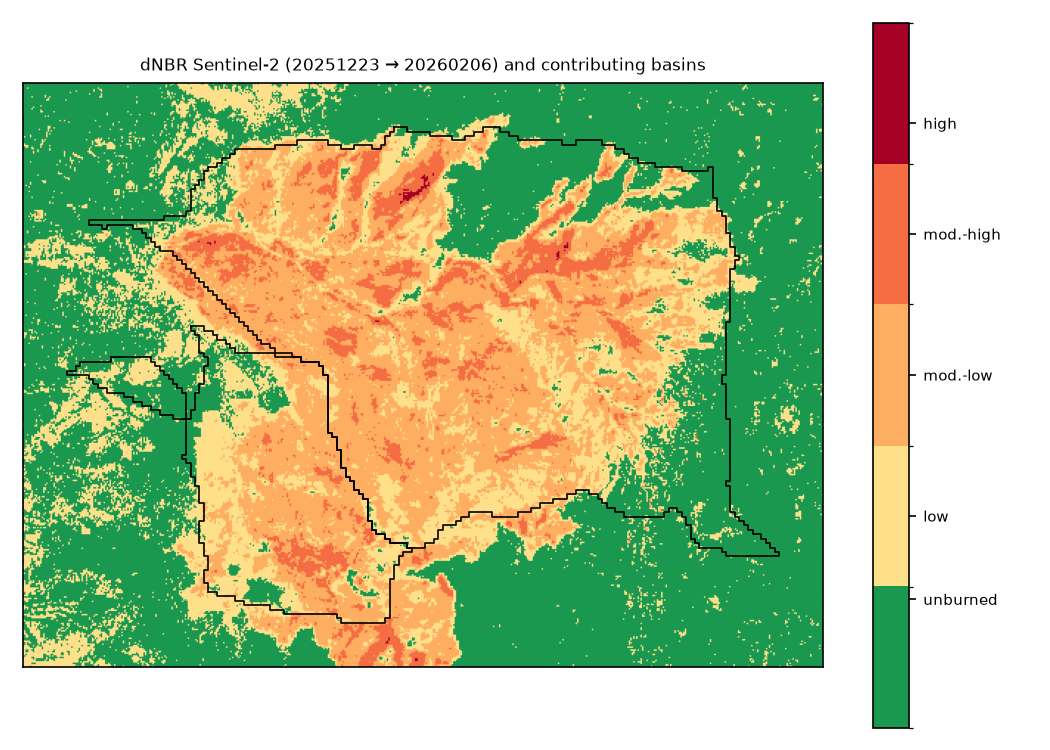
\includegraphics[width=.85\textwidth]{dnbr}\caption{Estimated severity of the December 2025 fire according to the Sentinel-2 differenced normalized burn ratio (dNBR) (23 December 2025 and 6 February 2026) and catchment boundaries calculated from the terrain (main channel to the north, southern branch and smaller ravines).}\label{fig:dnbr}\end{figure}

\subsection{Initial Screening with the Previous Terrain}\label{sec:res-calib}
\begin{table}[htbp]\centering\small
\caption{First model generation (9 October 2026), with the previous terrain of 1,103 buildings: fraction of control points with maximum simulated thickness greater than \SI{5}{cm}, by street, and maximum thickness within a radius of \SI{40}{m} of each site. Culvert capacities are assumed; they do not describe the real structure. H1: main-channel inflow onto the alluvial fan; H2: inflow at the culvert inlet; H3: inflow distributed among channels; H4: combined alluvial-fan and culvert-inlet inflows plus southern inflows; H5: H4 plus hillside rainfall. All simulations use Glenwood~2b, $C_v=0.40$ and $Q_p=\SI{250}{m^3/s}$, except d03 ($Q_p=\SI{100}{m^3/s}$). LP: La Plaza (Álvaro del Portillo--Camino El Alba); GB: General Blanche (San Carlos de Apoquindo--Las Condesas); CEA: Camino El Alba; QH: Quebrada Honda; LPS: La Plaza Sur; UCC: Clínica UC Christus; CUA: Clínica Universidad de los Andes; Duoc: Duoc UC campus; dPH: minimum mud distance to the intersection of General Blanche and Padre Hurtado.}\label{tab:hipotesis}
{\setlength{\tabcolsep}{4pt}\begin{adjustbox}{max width=\textwidth}\begin{tabular}{llrrrrrrrrr}\toprule
Hypothesis & $V$ (thousand \si{m^3}) & LP & GB & CEA & QH & LPS & UCC (\si{m}) & CUA (\si{m}) & Duoc (\si{m}) & dPH (\si{m})\\\midrule
H3 & 80 & 0.87 & 0.86 & 0.61 & 0.00 & 0.00 & 0.22 & 0.00 & 0.42 & 1,160\\
H1 & 150 & 0.91 & 0.92 & 0.85 & 0.00 & 0.00 & 0.42 & 0.00 & 0.55 & 366\\
H3 & 150 & 0.88 & 0.92 & 0.78 & 0.00 & 0.00 & 0.39 & 0.00 & 0.53 & 516\\
H3 & 300 & 0.91 & 0.93 & 0.96 & 0.00 & 0.00 & 0.42 & 0.00 & 0.54 & 4\\
H2 & 150 & 0.00 & 0.00 & 0.00 & 0.69 & 0.00 & 0.00 & 0.00 & 0.00 & 856\\
H4, $f_\mathrm{sup}=0.5$ & 150 & 0.88 & 0.88 & 0.57 & 0.66 & 0.00 & 0.26 & 0.00 & 0.46 & 1,007\\
H4, $f_\mathrm{sup}=0.9$ & 150 & 0.88 & 0.91 & 0.68 & 0.54 & 0.00 & 0.35 & 0.00 & 0.52 & 816\\
H5 (H4 + rainfall of \SI{20}{mm/h}) & 150 & 0.88 & 0.88 & 0.57 & 0.66 & 0.00 & 0.26 & 0.06 & 0.46 & 1,005\\
H1, carved channel, no model sink & 150 & 0.89 & 0.94 & 0.87 & 0.55 & 0.00 & 0.31 & 0.00 & 1.63 & 338\\
\quad same, assumed sink capacity \SI{10}{m^3/s} & 150 & 0.89 & 0.94 & 0.87 & 0.43 & 0.00 & 0.31 & 0.00 & 1.63 & 338\\
\quad same, assumed sink capacity \SI{30}{m^3/s} & 150 & 0.89 & 0.94 & 0.87 & 0.01 & 0.00 & 0.31 & 0.00 & 1.63 & 338\\
\bottomrule\end{tabular}\end{adjustbox}}
\end{table}

Table~\ref{tab:hipotesis} summarizes the screening simulations. Four patterns emerge from the simulations:
\begin{enumerate}
\item \textbf{Alluvial-fan corridors.} La Plaza, Mons.\ Álvaro del Portillo, Av.\ San Carlos de Apoquindo, upper General Blanche and Camino El Alba exceed the threshold at \SIrange{85}{100}{\percent} of their points in all hypotheses with outflow on the alluvial fan, for volumes between \SI{80000}{m^3} and \SI{300000}{m^3}. Duoc UC and Clínica UC Christus are reached in all of them, with thicknesses of \SIrange{0.4}{1.6}{m} and \SIrange{0.2}{0.4}{m}, respectively.
\item \textbf{Quebrada Honda.} In screening, this street exceeds the threshold only when simulated flow emerges at the surface at the Francisco Bulnes Correa culvert inlet. This occurs if a source is imposed there (H2, H4) or if the terrain represents the open channel conveying flow to the culvert inlet and the model sink does not remove it. In those tests, outflow there of \SI{8}{\percent} of the volume is sufficient.
\item \textbf{Assumed culvert capacity (previous terrain; superseded).} With the channel represented and only 1,103 buildings, \SI{12800}{m^3} reaches the culvert inlet, with a maximum discharge of \SI{16.5}{m^3/s}; in that scenario, the model sink with an assumed capacity of \SI{30}{m^3/s} or \SI{100}{m^3/s} removes it and Quebrada Honda remains dry (\SI{1}{\percent}). With the full city, this conclusion changes: the calculated discharge increases to about \SI{65}{m^3/s} and an assumed capacity of \SI{30}{m^3/s} leaves surface flow (Section~\ref{sec:res-colector}). With an assumed capacity of \SI{10}{m^3/s}, the model calculates an overflow of about \SI{2600}{m^3} and Quebrada Honda is wetted at \SI{43}{\percent} of its points (Table~\ref{tab:hipotesis}).
\item \textbf{Southern sector.} None of the simulations in Table~\ref{tab:hipotesis} wets Av.\ La Plaza Sur or the Universidad de los Andes campus. Only rainfall on the eastern hillside (H5) reaches Clínica Universidad de los Andes, with \SI{6}{cm} in its surroundings, consistent with the clinic's statement reported by Radio La Señal that the impact was outside \citep{radiolasenal2026}.
\end{enumerate}
With the previous terrain, no simulation meets the four acceptance criteria specified in advance (Section~\ref{sec:calib}). The sites criterion is not met in any simulation because the campus is not reached, and the reach criterion is not met in the \SI{150000}{m^3} simulations.

\begin{figure}[htbp]\centering
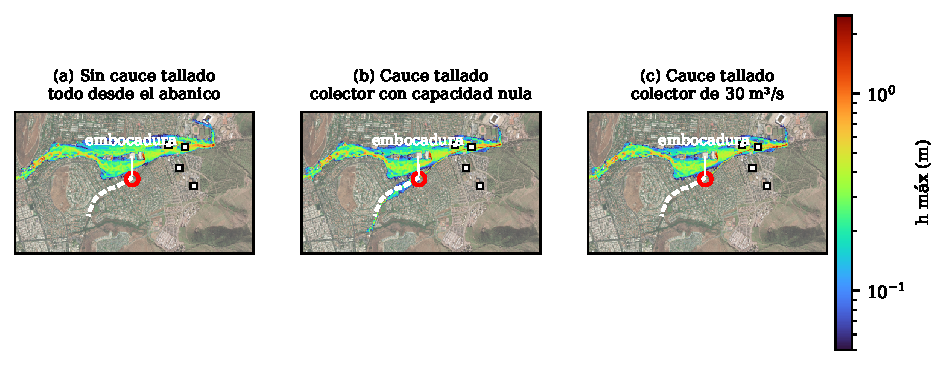
\includegraphics[width=\textwidth]{colector}
\caption{First model generation (previous terrain, 1,103 buildings; superseded by Section~\ref{sec:res-colector}). Maximum simulated thickness with \SI{150000}{m^3} emerging on the alluvial fan. (a) Base terrain: flow does not reach Quebrada Honda (dashed white line). (b) Carved linear-park channel and model sink with assumed zero capacity: flow reaching the culvert inlet through the channel (red circle) overflows toward Quebrada Honda. (c) Same terrain with an assumed sink capacity of \SI{30}{m^3/s}: the model removes the arriving flow and Quebrada Honda remains dry. Squares indicate sites with impacts reported by the sources in Section~\ref{sec:evidencia}.}\label{fig:colector}\end{figure}

\subsection{Comparison with Information Obtained after Formulation of the Hypotheses}\label{sec:res-contraste}
Three sources became available after the hypotheses were formulated, allowing a partial comparison that was not independent of the press:
\begin{itemize}
\item \textbf{Preliminary account collected by El Desconcierto} \citep{eldesconcierto2026}: the outlet reports an account from the presidential delegate about obstruction of the entrance to two parallel conduits on General Blanche and describes an interruption in the operation of the Francisco Bulnes Correa settling chamber; it also reports channel overflow on that street as described by Carabineros. These are accounts from the source. In the scenarios tested, representing surface inflows in both sectors allows flow on the alluvial fan and Quebrada Honda to be reproduced, without confirming those accounts or the condition of the structures.
\item \textbf{Sernageomin technical report on the 31 January 2026 debris flow} \citep{sernageomin2026reterm}: describes a single corridor from Parque San Carlos de Apoquindo, through the Universidad de los Andes sector, to Quebrada Honda at Francisco Bulnes Correa, continuing toward the Apoquindo ravine, Hospital Dipreca and Paul Harris. The report describes the channel parallel to Quebrada Honda as filled with mud after that event. This matches the channel path that the model needs to represent. The expanded domain of the current version already includes the continuation toward Dipreca and Paul Harris.
\item \textbf{Press map} \citep{chilevision2026mapa}: traces the centerlines of Camino El Alba, General Blanche and Quebrada Honda to Padre Hurtado as debris-flow routes. Along those full lines, the simulation considered in that comparison wets \SI{92}{\percent} of Camino El Alba, \SI{40}{\percent} of General Blanche and \SI{27}{\percent} of Quebrada Honda. Lower General Blanche, between Las Condesas and Padre Hurtado, is not reproduced: the simulated flow favors Camino El Alba along that stretch.
\end{itemize}

More data became available between 9 and 10 October and were compared without modifying the simulations:
\begin{itemize}
\item \textbf{Locations where mud or water entered.} Senapred includes Av.\ La Plaza Sur among the three most affected streets, according to El Dínamo \citep{eldinamo2026}; the Universidad de los Andes campus had mud and stranded people, and Clínica Universidad de los Andes had minor water ingress \citep{interferencia2026,cooperativa2026}, as recorded in the municipal assessment reported by CNN Chile \citep{cnnchile2026balance}. On the terrain with buildings, the main-channel simulation does not wet any of these three points. The simulation adding the southern branches and hillside rainfall gives \SI{0.14}{m} next to Clínica Universidad de los Andes and wets part of La Plaza Sur, but leaves the campus with \SI{1}{cm}. Both calculate depths next to Clínica UC Christus (\SIrange{1.13}{1.16}{m}, compared with about \SI{1}{m} reported in its emergency department \citep{cadena3_2026}) and the Duoc UC campus (\SI{1.9}{m}).
\item \textbf{31 January event.} According to T13, with \SI{75}{mm} in \SI{1}{h} \SI{20}{min}, a much greater intensity than on 8 October, it affected \SI{8}{ha}, about \SI{4}{km} of streets and 11 homes \citep{t13_2026mallas}, and the Francisco Bulnes Correa culvert ``worked very well'' according to the mayor \citep{latercera2026enero}. The difference between the reported assessments motivates scenarios of antecedent saturation and available material; it does not establish their contribution to the event or allow a causal comparison with peak intensity.
\item \textbf{Affected surface area.} The \SI{253}{ha} reported by Chicureo Hoy \citep{chicureohoy2026} matches the area of the municipal perimeter published by the press (calculated area: \SI{253.0}{ha}). It is a safety perimeter rather than a map of mud: simulated mud occupies about \SI{40}{ha} inside it, because it concentrates in the streets. It is not used to discriminate between hypotheses.
\item \textbf{Hospital de la FACh.} According to Interferencia, water was reported in its emergency department \citep{interferencia2026}. No simulation reaches that point, about \SI{1.3}{km} north of the flow path; it is not used as a fitting criterion. Urban rainfall drainage lies outside the model, and the origin of that impact is not inferred here.
\end{itemize}

\subsection{Indicators at Critical Sites}\label{sec:res-indicadores}
First model generation (previous terrain, simulation e04; not directly comparable with simulations with the full city). In the simulation with the carved channel and the culvert with assumed zero capacity, maxima within a radius of \SI{40}{m} are as follows:
\begin{itemize}
\item Duoc UC: \SI{1.6}{m} thickness, \SI{6.3}{m/s} and \SI{33}{kPa} dynamic pressure; the front arrives at minute~4.
\item Intersection of General Blanche and San Carlos de Apoquindo: \SI{1.4}{m}, \SI{6.7}{m/s} and \SI{37}{kPa}, at minute~7.
\item Clínica UC Christus: \SI{0.3}{m} and \SI{1.6}{m/s}, at minute~9.
\item Francisco Bulnes Correa culvert inlet: \SI{1.6}{m} and \SI{3.9}{m/s}, at minute~13.
\end{itemize}
Minutes are counted from the start of the pulse. In that scenario, 170 buildings have mud above \SI{5}{cm} next to their façades, 46 above \SI{0.5}{m} and 11 above \SI{1}{m}; 8 receive dynamic pressure greater than \SI{10}{kPa}. These values carry the screening bias already noted and have not been compared with measurements.


\IfFileExists{secciones/recorrido.tex}{\section{The Hypotheses, One by One}\label{sec:recorrido}
This section brings together in a single account what the preceding sections present separately. For each hypothesis, it indicates the observation that motivated it, how it was represented in the model, the results and its status at closure. Table~\ref{tab:recorrido} summarizes the account. A ``compatible'' result means that the model reproduces observations under reasonable assumptions; it does not prove that the event occurred that way. The exploratory compatibility index (ECI) compares hypotheses using the same criteria; it is not a validation.

\subsection{Flow Entry Points Tested in the Model}
\paragraph{H1: Assumed Main-Channel Discharge onto the Alluvial Fan.} \emph{Why it was proposed.} Initial reports collected by Chilevisión and Interferencia placed the origin in the ravine descending to the alluvial fan at Álvaro del Portillo, La Plaza and General Blanche, where the ravine enters a conduit beneath the developed area \citep{chilevision2026,interferencia2026}. The scenario assumes that the conduit receives no flow and assigns the entire inflow to the surface from that point. \emph{How it was represented.} A triangular mixture hydrograph injected at the channel outlet onto the alluvial fan. \emph{Results.} In the model with only the main channel (v01), mud travels along General Blanche and Camino El Alba and reaches close to Padre Hurtado, but it does not reproduce the reported impacts in the southern sector: Av.\ La Plaza Sur, Clínica Universidad de los Andes and the campus remain dry. In the test using held-out observations, it reaches the same 19 of 49 points as the selected hypothesis. \emph{Status.} Inflow through the main channel reproduces the northern branch in these scenarios; by itself it does not reproduce the reported impacts in the southern sector.

\paragraph{H2: Assumed Surface Inflow at the Francisco Bulnes Correa Culvert.} \emph{Why it was proposed.} Interferencia and BioBioChile collected accounts of an overflow where the enclosed channel crosses Francisco Bulnes Correa, at the start of Quebrada Honda, which is among the reported affected streets \citep{interferencia2026,biobio2026origen}. \emph{How it was represented.} A source at the culvert inlet (e03), and hypothetical scenarios of culvert capacity represented as a sink (v10, v11, v17, v18). \emph{Results.} A discharge only at the inlet reaches none of the 49 held-out points: by itself it does not reproduce the full set of observations. With assumed inflow from the alluvial fan, the city model channels about \SI{93000}{m^3} toward the inlet, with peaks near \SI{65}{m^3/s}. In those scenarios, which do not evaluate the real structure, the sink with an assumed capacity of \SI{30}{m^3/s} reaches that limit and simulated flow remains in Quebrada Honda. \emph{Status.} As a sole input, it does not reproduce observations under the assumptions tested. As a transit point for assumed flow from the alluvial fan, it reproduces flow in Quebrada Honda; it does not establish why that street was affected during the event.

\paragraph{H3: Inflow Distributed among Several Channels.} \emph{Why it was proposed.} Sites with reported impacts to the south (La Plaza Sur, the campus, Clínica Universidad de los Andes) are not reached in the model by inflow from the main channel. The mapping used also represents a southern branch reaching the campus and short ravines ending at La Plaza Sur. \emph{How it was represented.} The same hydrograph, distributed in proportion to each catchment's area: \SI{79.5}{\percent} to the main channel, \SI{18.8}{\percent} to the southern branch and \SI{1.7}{\percent} to the short ravines. \emph{Results.} Without hillside rainfall, the configuration with the official southern branch (v21) obtains an ECI of 68/100 and does not reach Clínica Universidad de los Andes. With rainfall on the hillside (H5, below), z02 obtains an ECI of 72/100 and was the hypothesis selected for the held-out test, whose outcome was unfavorable (19 of 49 points). \emph{Status.} It is the basis of all subsequent hypotheses, but by itself leaves much of the official affected area without mud.

\paragraph{H4: Combined Discharge.} \emph{Why it was proposed.} Initial results showed that Quebrada Honda became wet only if part of the simulated flow discharged at the inlet. \emph{How it was represented.} Inflows on the alluvial fan and at the inlet, plus the southern branches (e01 and g03). \emph{Results.} In screening with \SI{150000}{m^3}, Quebrada Honda is wetted at \SIrange{54}{66}{\percent} of its points, but the front remains \SIrange{816}{1007}{m} from Padre Hurtado (Section~\ref{sec:res-calib}). \emph{Status.} It does not meet the reach criterion in those tests.

\paragraph{H5: Rainfall on the Hillside.} \emph{Why it was proposed.} Initial results showed that Clínica Universidad de los Andes remained dry if mud arrived only through the channels. \emph{How it was represented.} H4 plus rainfall on the lower hillside in screening (f02 and f03); subsequently, distributed channels plus rainfall with the full city (v02 and z02). \emph{Results.} z02 obtains an ECI of 72 and reaches 19 of 49 facilities in the unfavorable held-out test. Without the assumed hillside rainfall (v21), the model does not reach Clínica Universidad de los Andes and the ECI falls to 68. \emph{Status.} Assumed rainfall on the lower hillside contributes to reproducing the reported impacts in the southern sector; the held-out test remains unfavorable. Its intensity is revisited below.

\subsection{How Much Mud, and of What Type}
\paragraph{Volume.} \emph{Why it matters.} In the model, reach depends on the assumed volume: with \SI{150000}{m^3}, the front stops \SI{348}{m} from Padre Hurtado; with \SI{300000}{m^3}, it reaches within \SI{100}{m}. \emph{How it was constrained.} Using estimates independent of the urban model (Section~\ref{sec:res-volumen}): a rainfall--runoff balance with soil saturation assumed from the information that about \SI{95}{mm} had fallen at Río Molina between 5 and 7 October \citep{cr2_2026} gives a median of \SI{295000}{m^3}. \emph{Status.} The input volume compatible with the simulated reach agrees in order of magnitude with the rainfall balance under its assumptions; it was not adjusted to make them agree.

\paragraph{Mud Concentration.} \emph{Why it matters.} Thicker mud stops sooner; more fluid mud travels farther and spreads out. \emph{Results.} In the model, thick mud (Glenwood~1) stops \SI{396}{m} from Padre Hurtado; very fluid mud (Aspen~2) obtains 70/100. Quadrature over concentration (Section~\ref{sec:res-posterior}) gives an expected area of \SI{169}{ha} (\SIrange{144.5}{192.3}{ha}) and an ECI between 71 and 73. \emph{Status.} Within the plausible range, concentration has little effect on the comparison between hypotheses.

\subsection{How the City Is Represented in the Model}
\paragraph{Channeling by the Represented Streets.} \emph{Why it was proposed.} The first terrain had 1,103 buildings; mud spread over the surface and did not reproduce the meter reported at Clínica UC Christus \citep{cadena3_2026}. \emph{Results.} With the 42,018 building footprints, mud flows deeper along the streets: next to Clínica UC Christus it rises from \SI{0.3}{m} to \SIrange{1.1}{1.2}{m}, and the culvert inlet receives seven times as much mud. \emph{Status.} Confirmed as a model effect: without the buildings, the reconstruction is not comparable with observations.

\paragraph{Mud Entry into the Represented Houses.} \emph{Why it was proposed.} After the held-out test, the diagnosis showed that the model left the interior of the affected strip dry: mud ran along the streets but did not enter lots, whereas the images consulted are interpreted as showing mud inside houses and courtyards. \emph{How it was represented.} Buildings in the official affected area with floors \SI{0.3}{m} above ground and high resistance, allowing mud to enter and retaining it (v26). \emph{Results.} The fraction of urban mud within the official affected area rises from 0.34 to 0.54, and the verified ECI reaches 76. With half the resistance, the result barely changes: what matters is that mud enters the lots. The tradeoff is the depth next to Clínica UC Christus, which falls to \SI{0.30}{m} because the represented upstream houses store mud in the model. Keeping large blocks solid and making only houses of \SI{250}{m^2} or less porous (d39) does not restore that depth (\SI{0.31}{m}): the effect comes from upstream storage, not building size.
\emph{Status.} It improves agreement with the official affected area, but is a fitting adjustment after the held-out test and has not been validated with new observations.

\subsection{The Universidad de los Andes Campus and La Plaza Sur}
\paragraph{Tested Inflows from the Avenue and Hillside.} \emph{Why it was proposed.} The Meganoticias video is interpreted as showing turbid water descending from the woodland and filling a sunken courtyard on campus (visually estimated depth: \SIrange{15}{35}{cm}) \citep{meganoticias2026uandes}, and El Dínamo reports that Senapred named La Plaza Sur among the most affected streets \citep{eldinamo2026}. The city model left that sector almost dry. \emph{What was tested.} First, assumed surface inflow at Álvaro del Portillo toward the campus: with none of the fluids tested, not even turbid water, does the simulated flow reach the courtyard, because the inflow point lies outside the local catchment delineated for the courtyard. Then, runoff from the hillside itself and from the hill, with features that the \SI{30}{m} terrain does not resolve: the low-lying roadway of La Plaza Sur, the passage from the clearing to the courtyard, and the dirt road on the hill. \emph{Results.} With those represented features, simulated water follows La Plaza Sur northward, enters through the clearing and fills the courtyard to \SIrange{0.12}{0.30}{m}, within the range visually estimated from the video, with assumed rainfall of \SIrange{15}{35}{mm/h}. \emph{Status.} The simulated La Plaza Sur $\rightarrow$ clearing $\rightarrow$ courtyard route is compatible with observations and persists at the rainfall intensities tested. The assumed inflow at Álvaro del Portillo does not reach the courtyard under the assumptions tested. With a fine mesh on the campus within the city simulation and measured rainfall (m36), the courtyard reaches \SI{0.17}{m} and La Plaza Sur is \SI{58}{\percent} wetted: the difference between scales was due to resolution.

\paragraph{More Fluid Flow on the Lower Hillside.} \emph{Why it was proposed.} The cited Meganoticias video is interpreted as showing turbid water, with no discernible urban debris; this motivates testing a more dilute flow on the lower hillside. \emph{Results.} With a lower concentration on the lower hillside, the campus also becomes wet with a fine time step and the verified ECI reaches 78. \emph{Status.} Compatible: the scenario with a more fluid mixture in the southern sector better reproduces the fitting observations; it does not determine the actual flow composition.

\paragraph{The \emph{Bike Park}.} \emph{Why it was proposed.} In the images consulted, the author identified a \emph{bike park} with bare-earth trails above the hill road; its representation was tested to examine the calculated route toward the road. \emph{Results.} With and without the main trail carved, results along the road, on La Plaza Sur, in the clearing and in the courtyard are identical (mrbc and mrbt): with this terrain, water was already draining toward the road. Including the entire area of the \emph{bike park} and upper hillside in the rainfall does increase water input (La Plaza Sur rises from \SI{69}{\percent} to \SI{78}{\percent} wetted). \emph{Status.} In the tests, carving the trail does not change the calculated route; including that area in the applied rainfall increases the model’s water input. Its possible sediment contribution cannot be evaluated with this model, which does not simulate erosion.

\subsection{The Integrated Hypothesis and Rainfall}
\paragraph{Integrated Hypothesis.} It combines the distributed channels, rainfall on the lower hillside, porous houses, more fluid flow on the lower hillside and campus features. With assumed rainfall of \SI{35}{mm/h} for one hour, it obtains 82/100, verified with a fine time step, and meets all four original criteria. With rainfall measured at Río Molina and its recorded temporal distribution, a pulse with a maximum of \SI{10.9}{mm} in \SI{30}{min} (p34b, corrected), it obtains 81/100; the campus reaches \SI{0.49}{m}, La Plaza Sur is wetted at \SI{33}{\percent} of its points and the area with more than \SI{5}{cm} is \SI{222}{ha}. With the same rainfall distributed uniformly over \SI{4}{h} (v33), it falls to 79/100.
\emph{Status.} It is the hypothesis most compatible with the fitting observations, but it was constructed after the held-out test: validating it requires new independent observations.

\paragraph{The Hypothetical Tree Obstacle.} \emph{Why it was proposed.} The author marked a line of trees descending along the main ravine and an accumulation at its end, shortly before the outlet onto the alluvial fan. An assumed obstacle was tested to examine whether the calculated flow is diverted southward. \emph{How it was represented.} A channel carved along the line of trees, with flow injected upstream, and the same channel with the accumulation represented as a \SI{3}{m}-high obstacle (arc and art). \emph{Results.} In the model, the assumed obstacle does not divert the flow southward: the Álvaro del Portillo sector and campus have the same wetted area with and without the assumed obstacle (\SI{20.2}{ha}). The model obstacle retains and spreads mud near the outlet onto the alluvial fan, and the mud travels less far westward. The ECI barely changes (78 versus 79). \emph{Status.} With this terrain, the assumed obstacle at the end of the line of trees does not reproduce the reported impacts in the southern sector.

\paragraph{The Fire.} \emph{Why it was proposed.} According to CR2, the December 2025 fire affected most of the catchment \citep{cr2_2026}. The literature cited in the severity analysis describes possible increases in runoff (hydrophobic soil without cover) and available loose material after fires. \emph{How it was quantified.} Using severity estimated by satellite (dNBR, Section~\ref{sec:res-incendio}): \SI{82}{\percent} of the contributing catchments shows a burn signal, but only \SI{10}{\percent} at moderate-high or high severity. With that severity and the assumed coefficients, the balance for the scenario without fire gives a mud pulse of about \SI{62}{\percent} of the volume with fire (between \SI{51}{\percent} and \SI{76}{\percent}), with \SI{43}{\percent} of the solids. The empirical Staley M1 model gives a median probability of 0.28 with fire versus 0.07 without it, as an illustrative application. \emph{Results in the city.} With the volume without fire (f35b and f38b, corrected), mud wets \SIrange{179}{193}{ha}, compared with \SI{222}{ha} in p34b (\SIrange{13}{19}{\percent} less), reaches fewer streets (0.70--0.73 versus 0.77) and leaves a smaller thickness at Clínica UC Christus (\SIrange{0.19}{0.23}{m} versus \SI{0.30}{m}). However, the ECI does not fall (80--82), because it rewards the fraction of mud within the official affected area, which rises when there is less mud. \emph{Status.} With the assumed coefficients, the scenario with fire calculates a greater volume and, above all, more solids and a higher empirical probability of debris flow. With these metrics, the urban model does not support a claim that this additional volume was necessary to reproduce observations.

\subsection{Aspects Untested at Closure}
The full list appears under ``What Remains Unproven'' (Section~\ref{sec:conclusiones}); three limitations are highlighted here.
\begin{itemize}
\item \textbf{Independent validation.} Everything after the held-out test concerns fitting. Its independent validation remains untested: the integrated hypothesis was not compared with new observations, such as post-event radar images or official high-water marks.
\item \textbf{Clínica UC Christus.} No configuration simultaneously reproduces the meter reported there and the extent within the official affected area.
\item \textbf{What the model does not simulate:} erosion and deposition along the flow path, logs and vehicles swept away, urban drainage, infiltration within the city and changes in flow concentration.
\end{itemize}

\begin{table}[htbp]\centering\small
\caption{Summary of the modeling hypotheses: what motivated them, what was calculated and their status within the tests. ECI: exploratory compatibility index (a comparison of fit, not a measure of predictive accuracy); QH: Quebrada Honda. Compatibility refers to the model; it does not identify causes of the event.}\label{tab:recorrido}
\begin{adjustbox}{max width=\textwidth}\begin{tabular}{@{}>{\raggedright\arraybackslash}p{.17\textwidth}>{\raggedright\arraybackslash}p{.27\textwidth}>{\raggedright\arraybackslash}p{.30\textwidth}>{\raggedright\arraybackslash}p{.22\textwidth}@{}}\toprule
Hypothesis & Motivating information & Model result & Status in the model\\\midrule
H1 main channel & Origin reported on the alluvial fan (press cited in H1) & Reproduces the northern branch; not the southern sector & Insufficient by itself\\
H2 Francisco Bulnes Correa culvert & Overflow reported at the start of Quebrada Honda (press cited in H2) & As sole input, 0 of 49 points; as a flow passage, reproduces Quebrada Honda & Insufficient as sole input\\
H3 distributed inflow & Southern sector outside the main channel & ECI 68 without rainfall (v21); 72 with rainfall (z02, H5) & Basis of subsequent hypotheses\\
H4 combined discharge & Quebrada Honda dry in the model without inflow at the inlet & Screening: QH \SIrange{54}{66}{\percent}; front \SIrange{816}{1007}{m} from Padre Hurtado & Does not meet reach criterion\\
H5 hillside rainfall & Clínica Universidad de los Andes dry in the model without rainfall & ECI 72 (z02); without rainfall, 68; held-out test 19/49 & Compatible fit; unfavorable test\\
Volume & Reach to Padre Hurtado & Assumed \SI{300000}{m^3}, of the order of the balance with saturated soil & Consistent\\
Buildings & Meter reported by Cadena 3 at Clínica UC Christus & Represented streets channel simulated mud & Confirmed in the model\\
Porous houses & Interior of the official affected area dry in the model & ECI 76; Clínica UC Christus falls to \SI{0.30}{m} & Unvalidated fit\\
Campus via La Plaza Sur & Meganoticias video; Senapred according to El Dínamo & Courtyard \SIrange{0.12}{0.30}{m} via the clearing; m36: \SI{0.17}{m} and La Plaza Sur \SI{58}{\percent} & Compatible\\
Overflow from Álvaro del Portillo to campus & Assumed overflow location & Does not reach the courtyard with the fluids tested & Not reproduced in the tests\\
\emph{Bike park} & Bare trails above the road & Carving the trail does not change the simulated route; assumed rainfall on its area adds water & No effect on the simulated route\\
Integrated hypothesis & All of the above & ECI 79--82 depending on rainfall & Best fit, unvalidated\\
Tree obstacle & Line of trees and accumulation identified in images & Does not divert flow southward; retains mud near the alluvial fan & Does not reproduce the southern sector\\
Fire & Fire reported by CR2 nine months earlier & Scenario without fire: about \SI{62}{\percent} of the volume, \SI{43}{\percent} of the solids and about 4-fold lower illustrative model probability; in the city, \SIrange{13}{19}{\percent} less area, ECI 80--82 versus 81 & Sensitivity to assumptions\\\bottomrule
\end{tabular}\end{adjustbox}
\end{table}
}{}

\section{Discussion}\label{sec:discusion}
\paragraph{What the Model Reproduces.} With the full city, the configuration selected for the held-out test (z02) reproduces the two corridors delimiting the official affected area---Camino El Alba and General Blanche to the north, Quebrada Honda to the south---the reach to Av.\ Padre Hurtado, and the reported impacts near Duoc UC and Clínica Universidad de los Andes. It calculates about one meter of mud next to Clínica UC Christus, comparable in magnitude to the depth reported in its emergency department \citep{cadena3_2026}. The input volume that reproduces that reach in the model, about \SI{300000}{m^3}, agrees with the independently obtained estimate from reported rainfall, assuming saturated soil and rain falling across the entire catchment surface. Agreement between estimates obtained through different procedures supports the consistency of the order of magnitude, under their respective assumptions; it does not constitute independent validation.

\paragraph{Antecedent Rainfall, Isotherm and Volume.} According to T13, \SI{75}{mm} fell in \SI{80}{min} on 31 January, and its impact assessment was smaller than those reported for October \citep{t13_2026mallas}. The intensities reported for October are lower; the mayor reported about \SI{144}{mm} of accumulated rainfall \citep{interferencia2026} and CR2 placed the \SI{0}{\celsius} isotherm above the catchment summit \citep{cr2_2026}. This information motivates scenarios with different assumptions about saturation and the area receiving rainfall; the comparison does not establish the cause of the event or the relative contribution of those factors. Under the calculation assumptions, the upper bound on the snowmelt contribution is below \SI{5}{\percent}: no snow was detected in the cloud-free part of the catchment in the Sentinel-2 image of 21 September.

\paragraph{The Role of Drainage (Hypothetical Scenarios).} In the scenarios tested, the impact on Quebrada Honda is reproduced when part of the calculated flow is not removed by the model sink representing the Francisco Bulnes Correa culvert. With the full city, the calculated discharge at the culvert inlet reaches about \SI{65}{m^3/s}; under the assumptions tested, an assumed capacity of \SI{30}{m^3/s} leaves surface flow, and the analysis places the calculated threshold of assumed capacity for removing it entirely near \SI{65}{m^3/s}, with capture of the entire cross section in the model. These values do not describe the real structure. Official hydrographic mapping represents channel continuity along Quebrada Honda downstream of the culvert inlet; in the simulations, flow not removed by that sink continues along that alignment. The analysis constrains assumed capacities under the model assumptions; it does not determine the capacity, condition or operation of the real structure during the event and does not allow responsibility to be attributed.

\paragraph{Possible Explanations for the Simulated Extent outside the Official Affected Area.} In z02, only one third of the simulated urban mud falls within the official affected area; with porous houses (z26), the fraction rises to 0.54, and with the corrected integrated hypothesis and measured rainfall (p34b), to 0.48. The reference is the official affected area, which is a management perimeter rather than a verified mud footprint. The following representations were tested; their results describe model sensitivity and their correspondence with the event remains unproven:
\begin{enumerate}
\item \textbf{Impermeable buildings.} In the initial configuration each building is a solid block; the press sources collected in the account report mud entering homes. Entry and retention within lots through porous buildings, a representation commonly used in urban flooding \citep{schubert2012}, were tested as an alternative assumption (v26, verified with a fine time step in z26). The fraction within the official affected area rises from 0.34 to 0.54, but the depth next to Clínica UC Christus falls to \SI{0.30}{m}.
\item \textbf{Coarse load.} The images consulted, described in the theoretical framework, show stones, logs and entrained vehicles. Fine-matrix rheology does not include that additional resistance; a slightly more concentrated mud mixture ($C_v=0.43$, between the one that extends too far and the one that falls short) represented it in a simple way (v25), without reducing the extent outside the official affected area (fraction inside: 0.346 versus 0.344 in z02).
\item \textbf{Vegetation and gardens.} FABDEM removes trees and roughness outside streets is moderate; increasing it (v27) raises the fraction within the official affected area to 0.388.
\end{enumerate}
There is also a limitation of the metric: the model does not distinguish rainwater from debris-flow mud, so rainfall runoff in other neighborhoods counts as mud outside the official affected area and penalizes hypotheses with hillside rainfall.

\paragraph{Sensitivity to Terrain.} In the tests, explicit representation of smaller channels is the factor that most changes the calculated flow path: carving the linear-park channel modifies the presence of simulated flow in Quebrada Honda, the assumed southern-branch alignment modifies its arrival at upper Álvaro del Portillo, and the representation of the culvert inlet changed Quebrada Honda coverage by \SI{44}{\percent}. With \SI{30}{m} terrain, these corridors must be carved from mapping; the official hydrographic network at 1:25,000 scale proved more reliable than OpenStreetMap for the southern branch.

\paragraph{Campus and Sunken Courtyard.} The simulated overflow at Álvaro del Portillo descends toward General Blanche and does not reach the courtyard with any of the fluids tested. The variants with local runoff, a more fluid mixture and representation of the clearing and lower roadway of La Plaza Sur were completed: the micro-simulations and m36 reproduce entry along La Plaza Sur $\rightarrow$ clearing $\rightarrow$ courtyard. With a fine mesh, m36 calculates \SI{0.17}{m} in the courtyard and wets \SI{58}{\percent} of La Plaza Sur (Section~\ref{sec:res-posterior}). This result is compatible with the images consulted, but does not identify the process that occurred during the event or constitute independent validation.

\paragraph{Test Using Held-Out Observations.} The only test using held-out observations, defined before comparing them with the model, had an unfavorable outcome: the selected hypothesis reaches 19 of 49 held-out affected facilities (\SI{39}{\percent}), compared with the specified \SI{70}{\percent}, and does not outperform the main-channel-only hypothesis (Section~\ref{sec:res-ronda}). The ECI of 72/100 measures compatibility with observations used to formulate the hypotheses; this test shows that such compatibility does not transfer to the fine spatial distribution of official impacts. The model also leaves substantial parts of the official affected area without mud, as well as exceeding its extent. This may be due to terrain resolution, building representation, volume or its temporal distribution, unmodeled local inflows, or differences between the definition of impacts in the official layer and the modeled depth threshold. Building representation, local resolution, volume and the temporal distribution of rainfall were tested subsequently (Section~\ref{sec:res-posterior}); those fits do not change the outcome of the held-out test and their independent validation remains untested.

\paragraph{What Improved after the Test.} Two changes in representation explain most of the improvement following the held-out test. First, allowing mud to enter lots redistributes the mixture within the official affected area. Second, the model assumes turbid water on campus and on La Plaza Sur and thick mud in the main branch, and represents the roads and confined roadways that convey it. Both have observational support (videos, Street View, Google Earth). Even so, they were chosen with knowledge of the results, so the increase in ECI (from 72 to 76--82 in fits verified with a fine time step) measures an improved fit, not validation. At closure, the integrated hypothesis obtains 79--82: 82 with an assumed \SI{35}{mm/h} and a fine time step (z32), 81 with the pulse measured at Río Molina (p34b, corrected) and 79 with that rainfall distributed over \SI{4}{h} (v33). With this representation of retention within lots, the calculated street depth next to Clínica UC Christus falls below the depth reported inside the clinic; this comparison does not establish actual storage within lots.

\paragraph{Fire and Metrics.} Severity estimated with dNBR (23 December 2025 and 6 February 2026) yields \SI{82}{\percent} with a burn signal and \SI{10}{\percent} with moderate-high or high severity; with the latter fraction, the Gartner median is \SI{148000}{m^3}. With the assumed coefficients, the balance without fire calculates about \SI{62}{\percent} of the volume and \SI{43}{\percent} of the solids; Staley M1 yields 0.28 with fire versus 0.07 without it, as an illustrative application. The corrected runs f35b and f38b wet \SIrange{179}{193}{ha}, compared with \SI{222}{ha} in p34b (\SIrange{13}{19}{\percent} less), and calculate \SIrange{0.19}{0.23}{m} next to Clínica UC Christus. The ECI of 80--82, compared with 81, shows that this index does not distinguish these scenarios (Section~\ref{sec:res-incendio}).

\paragraph{Validity.} The available observations are qualitative: streets and facilities reported by the press and authorities, and an official perimeter delimiting the management area rather than the area with verified mud. No published discharge measurements or high-water marks were located in the sources consulted. The exploratory compatibility index summarizes four criteria specified before simulation and serves to compare hypotheses with one another; it is not a measure of predictive accuracy, and differences of two or three points should not be interpreted as conclusive evidence that one hypothesis is superior to another.


\paragraph{Confidence by Result.} Instead of reducing results to a single indicator, Table~\ref{tab:confianza} assigns each a qualitative confidence assessment at closure.
\begin{table}[htbp]\centering\small
\caption{Qualitative assessment of confidence in each result at closure, conditional on assumptions and available evidence.}\label{tab:confianza}
\begin{tabular}{p{0.42\textwidth}p{0.5\textwidth}}\toprule
Result & Confidence level\\\midrule
General simulated mud corridors & Relatively high: compatible with multiple scenarios and the official affected area\\
Need to represent channels and transitions to culverts & Robust finding of model sensitivity\\
Order of magnitude of estimated mixture volume & Conditional estimate, with a wide range (\SIrange{181000}{468000}{m^3})\\
Actual culvert capacity & Not determined; only capacities tested in hypothetical scenarios\\
Calculated depth in front of buildings & Exploratory, dependent on terrain and parameters\\
Velocities, pressures and arrival times & Calculated indicators, without instrumental validation\\
\bottomrule\end{tabular}
\end{table}


\section{Directions for Further Investigation}\label{sec:profundizacion}
The study is closed. These seven topics distinguish completed tests from aspects untested at closure, collected under ``What Remains Unproven'' (Section~\ref{sec:conclusiones}):
\begin{enumerate}
\item \textbf{Burn severity and speed of runoff concentration.} Sentinel-2 dNBR was calculated using scenes from 23 December 2025 and 6 February 2026: \SI{82}{\percent} of the catchments shows a burn signal and \SI{10}{\percent} has moderate-high or high severity. That estimate was incorporated into the balance with assumed runoff coefficients by severity and into the model of \citet{gartner2014}, whose median mixture volume became \SI{148000}{m^3} (Section~\ref{sec:res-incendio}). Runoff increases and the time of concentration of each subcatchment by severity remain untested; the hydrograph rise time to peak remains assumed (\SI{10}{min}).
\item \textbf{Higher-resolution terrain on the campus.} The micro-simulations and m36 reproduced entry through the clearing into the courtyard; m36 calculates \SI{0.17}{m}. The actual geometry of embankments, paths and access points remains unverified by a local LiDAR or photogrammetric survey, which was unavailable in this study.
\item \textbf{Separating rainwater from mud.} Untested: a passive tracer marking the fluid from the hydrographs would allow the perimeter to be evaluated using only that contribution, without counting urban rainfall runoff.
\item \textbf{Porous buildings and coarse load.} Mud retention in homes and additional resistance were tested in a simplified way (v25--v27; porosity verified in z26). Their calibration using damage information by dwelling remains untested; stones, logs and vehicles were not simulated as transported load.
\item \textbf{Independent validation.} Untested for fits made after the held-out test. The facilities test was performed and had an unfavorable outcome (19/49); the fits were not compared with Sentinel-1 radar, official deposit surveys or high-water marks.
\item \textbf{Concentration as a random variable.} Concentration was treated as uncertain through $C_v=0.20+0.30X$ with $X\sim\mathrm{Beta}(3,2)$ (mode 0.40 and mean 0.38), and propagated using five Gaussian nodes (q1--q5). An expected area of \SI{169}{ha} and an ECI between 71 and 73 were obtained (Section~\ref{sec:res-posterior}). Alternative distributions and the estimation of inundation probabilities and extreme percentiles remain untested. Three precautions remain. The distribution, constructed from literature ranges and event evidence, is a belief distribution rather than the actual statistical distribution of sediment, so its results are conditional on it and comparison with alternatives (uniform, Beta(2,2)) was not tested. Quadrature estimates moments well but not inundation probabilities or extreme percentiles, because wetting and drying introduce discontinuities, which can be handled by interpolating between simulations the threshold concentration at which each cell exceeds a given thickness, or with more simulations (Latin hypercube sampling). Varying concentration between simulations represents uncertainty in a parameter, which is a different level of modeling from the physical evolution of concentration along the flow path.
\item \textbf{Evolution of concentration.} Erosion, deposition and incorporation of debris change concentration along the flow path. Untested: an input sediment hydrograph (a more concentrated front and a more dilute tail) and a concentration tracer transported with the flow would allow yield stress and viscosity to vary with it. This distinguishes the final deposit from the maximum flow extent, which is the only one reported at closure.
\end{enumerate}


\section{Conclusions and Closure of the Study}\label{sec:conclusiones}
This study closes with the version dated 13 October 2026. The following conclusions do not establish what happened or why. They describe what the results of a numerical model suggest, given the input parameters declared in this document and the 84 completed simulations: 19 screening runs with the previous terrain, 41 with the full city, 5 concentration quadrature runs and 19 campus micro-simulations. With different input data, another model or new observations, the results may change.

\subsection*{What the Results Suggest}
\begin{enumerate}
\item \textbf{General structure.} With the full city and the assumptions adopted, the model reproduces the Camino El Alba, General Blanche and Quebrada Honda corridors that delimit the official affected area, and the reach to Padre Hurtado. It does not reproduce the spatial distribution of impacts within that area: the test using held-out observations, defined before examining the results and performed only once, had an unfavorable outcome (19 of 49 facilities, compared with the specified \SI{70}{\percent}).
\item \textbf{Volume.} In the scenarios tested, about \SI{300000}{m^3} of mixture allows the observed reach to be reproduced. This is the same order of magnitude as an independent rainfall-balance estimate adopting the reported soil saturation. Neither value is a measurement.
\item \textbf{Flow inputs to the model.} Scenarios in which mud emerges at a single point do not reproduce the full set of observations. The most compatible scenarios combine inflow through the main channel, which reproduces the northern branch in the model, with the southern branch and assumed hillside rainfall, which reproduce part of the reported impacts in the southern sector.
\item \textbf{Role of the city.} Representing the 42,018 buildings changes the result: in the model, streets concentrate the flow and increase depths.
\item \textbf{Drainage.} The capacity scenarios for the Francisco Bulnes Correa culvert are hypothetical. In the model, with the assumed volume, a calculated discharge of the order of \SI{65}{m^3/s} reaches the inlet. With lower assumed capacities, flow continues over the surface along Quebrada Honda. These scenarios do not describe the real structure, for which public information on capacity, cross section and condition was unavailable. They do not support claims that the structure was obstructed, that it malfunctioned or that a different capacity would have changed what happened.
\item \textbf{Universidad de los Andes campus.} In the simulations, the assumed turbid-water inflow from the hillside and hill follows La Plaza Sur and enters a sunken courtyard through a clearing; this calculated route is compatible with the images consulted. With a fine mesh (m36), the calculated depth in the courtyard reaches \SI{0.17}{m}, within the range estimated from the published video, and La Plaza Sur is wetted at \SI{58}{\percent} of its points. The simulated overflow from Álvaro del Portillo does not reach that courtyard with this terrain.
\item \textbf{Fire.} According to the severity estimated with Sentinel-2, \SI{82}{\percent} of the contributing catchments shows a burn signal and \SI{10}{\percent} has moderate-high or high severity. With the assumed coefficients, the balance without fire yields about \SI{62}{\percent} of the mud volume and \SI{43}{\percent} of the solids of the scenario with fire. Staley M1, used illustratively, yields a median probability of 0.28 with fire versus 0.07 without it. In the city, the corrected runs without fire (f35b and f38b) wet \SIrange{179}{193}{ha}, compared with \SI{222}{ha} in p34b (\SIrange{13}{19}{\percent} less), and calculate \SIrange{0.19}{0.23}{m} next to Clínica UC Christus. The ECI remains at 80--82, compared with 81 with fire, and does not distinguish these scenarios.
\item \textbf{Best fit.} The integrated hypothesis obtains an exploratory compatibility index (ECI) of 79--82/100: 82 with an assumed \SI{35}{mm/h} and a fine time step (z32), 81 with the pulse measured at Río Molina (p34b, corrected) and 79 with that rainfall distributed over \SI{4}{h} (v33). It combines distributed channels, rainfall on the lower hillside, houses that allow mud to enter, turbid water on the lower hillside and campus features. It is a fit made after the held-out test: it is not validated and the index is not a measure of accuracy.
\item \textbf{Hypotheses unsupported by the model.} In the tests, carving the \emph{bike park} trail does not change the calculated water route, and an assumed log obstacle at the end of the tree line does not divert the simulated flow southward.
\end{enumerate}

\subsection*{What Remains Unproven}
\begin{itemize}
\item \textbf{Independent validation.} No hypothesis developed after the held-out test was compared with new observations, such as Sentinel-1 radar, high-water marks or depths measured in the field.
\item \textbf{Rainfall in the catchment.} No rain gauge within the catchment was identified in the sources consulted. The Río Molina station, about \SI{7}{km} away, was used with an assumed time offset.
\item \textbf{Actual flow volume and composition.} No measurements of the mobilized volume, its concentration or its rheology were located in the sources consulted. Alternatives to the Beta(3,2) distribution used in the quadrature, and the estimation of inundation probabilities and extreme percentiles, remain untested.
\item \textbf{Drainage structures.} The actual capacity, cross section and condition of the culvert and conduits are unknown. The study's scenarios do not evaluate them.
\item \textbf{Clínica UC Christus.} No configuration reproduces both the reported depth of about \SI{1}{m} \citep{cadena3_2026} and the extent within the official affected area. Calibration of retention in homes using damage information by dwelling remains untested.
\item \textbf{Terrain.} The \SI{30}{m} elevation model does not resolve roadways, curbs or narrow passages. The carved features are coarse representations based on supplied observations. No LiDAR terrain model was available.
\item \textbf{Processes not simulated:} erosion and deposition along the flow path, entrained logs and vehicles, urban drainage, infiltration within the city and changes in flow concentration. The tracer that would separate hydrograph inflow from rainfall, the sediment hydrograph and concentration transport remain untested.
\item \textbf{Fire parameters.} Runoff increases by severity are assumed; their local calibration and the time of concentration of each subcatchment by severity remain untested. Severity thresholds and empirical volume and probability models were calibrated outside Chile.
\item \textbf{Hypothetical tree obstacle.} Only one assumed location and height were tested, on the available terrain. It was not verified in the field.
\end{itemize}

\subsection*{Nature and Scope of This Study}
This document is an independent technical exercise for academic and public-information purposes, undertaken on personal initiative and not commissioned by third parties. It is not an expert assessment, an expert report, an official technical opinion or an evaluation of the structures, services or decisions of any person or institution. It is based exclusively on public information consulted between 8 and 13 October 2026, recorded with dates and hashes in the evidence log. The author has no direct knowledge of the events beyond these sources.

The results are responses of a numerical model to declared input parameters and explicit assumptions, several of them hypothetical. No calculated figure is a measurement, and no statement in this document asserts the cause of the event or attributes responsibility. References to structures, services or institutions concern model scenarios or what the cited sources reported, with attribution. The sources disagree on several points, and those discrepancies are presented without resolving them.

The study is closed as of this version. The code, derived data and frozen versions are available for review and reproduction. Any use of these results in technical, administrative or judicial decisions requires an independent professional assessment, with design information, inspection and field measurements.


\section*{Data and Code Availability}
The programs (\nolinkurl{prep.py}, \nolinkurl{sim.py}, \nolinkurl{calibrar.py}, \nolinkurl{verif_parada.py}, \nolinkurl{cuenca.py}, \nolinkurl{volumen_previo.py}), the evidence log of source consultations with their SHA-256 hashes, and the results are available at \url{https://aluvion.hirely.cl/datos.html}. The technical review reports are published in full on the same site.

\section*{Statement on the Use of AI Tools}\label{sec:declaracion-ia}
\section*{Version Control}\phantomsection\label{sec:versiones}
\begin{itemize}
\item \textbf{9 October 2026 (first model generation):} previous terrain with 1,103 buildings; screening of hypotheses H1--H4, carved linear-park channel and initial culvert tests (runs d, e, f, g, k and s). Its results for assumed culvert capacities were superseded by the version with the full city.
\item \textbf{10 October:} full city with 42,018 buildings and expanded domain (v01--v03, v05--v09, z01); volume with saturated soil, isotherm and Sentinel-2; comparison with the press.
\item \textbf{10 and 11 October:} model sink representing the culvert and capturing the entire cross section (v10, v11, v17, v18), Quebrada Honda and southern branch according to the official hydrographic network (v14, v15, v19--v21), fine-time-step check of the main hypothesis (z02).
\item \textbf{11 October, morning:} official affected area from IDE Chile as reference, exploratory compatibility index, maximum catchment elevation corrected in the text (\SI{2355}{m}), citations to the original CR2 analysis, distinction between observed and calculated results and hypothetical scenarios, and appendix of fact sheets.
\item \textbf{11 October, afternoon:} tests v25--v29, campus micro-simulations, protocol amendment~1 (tie-breaking rule) and test using held-out observations (unfavorable).
\item \textbf{12 October, early morning:} tests following the held-out test: porous houses (v26, v30, z26), verified more fluid flow on the lower hillside (z29), concentration quadrature (q1--q5), campus and La Plaza Sur micro-simulations with observations supplied by the author (mw10, mwq20, mrt10, mrp10, mrc10, mrd10) and integrated hypothesis (v32, verified with a fine time step in z32; v31 discarded), rainfall sensitivity (v33 with measured rainfall; micro-simulations at \SI{15}{mm/h} and \SI{25}{mm/h}; mrdn, mrds2).
\item \textbf{12 and 13 October (version 13a):}
\begin{itemize}
\item new sections: account of the events and explanation of each hypothesis;
\item Río Molina rainfall at \SI{30}{min} intervals (p34);
\item estimated burn severity from dNBR and response of volume and city scenarios (f35, f38);
\item \emph{bike park} (mrbc, mrbt), hypothetical tree obstacle (arc, art) and size-based porosity (d39);
\item correction of the 6 and 7 October rainfall at Tobalaba;
\item detection and correction of a numerical mass artifact (Section~\ref{sec:res-posterior}).
\end{itemize}
\item \textbf{13 October, afternoon (this version):} corrected repeat runs with measured rainfall and for the scenarios without fire (p34b, f35b, f38b), confirming the results: p34b obtains ECI 81, campus \SI{0.49}{m}, La Plaza Sur \SI{33}{\percent} and \SI{222}{ha}; f35b/f38b, \SIrange{179}{193}{ha}, Clínica UC Christus \SIrange{0.19}{0.23}{m} and ECI 80--82. The city simulation with a fine mesh on campus (m36) calculates \SI{0.17}{m} in the courtyard and wets \SI{58}{\percent} of La Plaza Sur. Closure of the study on 13 October 2026.
\end{itemize}
Table~\ref{tab:catalogo} records the completion dates of 65 runs: 19 screening runs, 41 full-city runs and 5 quadrature runs. The 19 campus micro-simulations are summarized in Sections~\ref{sec:res-ronda} and~\ref{sec:res-posterior}, but have no rows in that catalog.


\subsection*{Frozen Versions, Experiment Log and Held-Out Observations}
\begin{itemize}
\item \textbf{Frozen versions.} Each published version of the paper and sub-study is preserved as published, with its SHA-256 hash and a version-control tag (\url{https://aluvion.hirely.cl/paper/versiones/}). The main link points to the latest version without deleting earlier ones. Terrain files are not modified after use: each variant has its own file.
\item \textbf{Experiment log.} The log includes all runs, including stopped and canceled runs, runs ending in errors, and discarded runs, with their parameters, terrain, code version and reason. Discarded cases include: the transmissive boundary that created mass, the photogrammetric terrain with spurious depressions, v20 because of a threshold artifact, the \SI{12}{m} capture radius and v22--v24. At closure on 13 October, 84 simulations had been completed: 19 screening runs, 41 full-city runs, 5 concentration quadrature runs and 19 campus micro-simulations. The total of completed runs does not equal the number of accepted configurations; discard statuses are retained in the log.
\item \textbf{Separation of observations.} There are three groups:
  \begin{itemize}
  \item \emph{fitting observations}: streets, facilities, reach and perimeter (press and official affected area), thickness at Clínica UC Christus and campus accounts. These were used to formulate and select hypotheses, so the ECI measures compatibility, not validation;
  \item \emph{descriptive comparison}: affected properties and street centerlines from IDE Chile, and housing assessments. These have already been consulted, but did not enter the index or selection;
  \item \emph{held-out observations}: the 49 affected facilities from IDE Chile that do not coincide with fitting facilities were used only once in the unfavorable test (19/49). Comparison with post-event Sentinel-1 images and official high-water marks or depths was not tested; it was not used to validate subsequent fits (Section~\ref{sec:conclusiones}).
  \end{itemize}
\item \textbf{Preregistered test.} The metric for the facilities test was specified before comparison with the model: sensitivity with $h>\SI{5}{cm}$ within \SI{15}{m}, and a favorable outcome requiring a value of at least 0.70 and higher than those of two reference simulations (v01 and e03). The candidate z02 was chosen using only fitting observations and frozen before the test, which was performed once and had an unfavorable outcome (19/49, compared with the specified \SI{70}{\percent}; Section~\ref{sec:res-ronda}). The test is only partially independent, because the points lie within the official affected area used in the index, and does not replace independent scientific validation.
\end{itemize}

Artificial intelligence tools were used to support technical and editorial review. Two rounds of physics and mathematics review (A1 and A2) and one round of format review (F1) were completed using the gpt-6-astra language model (Codex). The available reports and the changes made are documented alongside the manuscript. Responsibility for the content rests with the author.


\bibliographystyle{apacite}\bibliography{referencias}
\clearpage\appendix
\section{Appendix: simulation catalog and fact sheets}\label{sec:anexo}

Table~\ref{tab:catalogo} lists the 65 screening, full-city and quadrature simulations; the 19 campus microsimulations are described in the text. Each key simulation then has a fact sheet with its figure: simulated mud (maximum thickness) over the official affected area from IDE Chile and the affected street centerlines, what it tests, what it shows, what limitations it has and what hypotheses it raises. Tests v25 to v29 and the campus microsimulations are summarized in Sections~\ref{sec:res-ronda} and~\ref{sec:res-posterior}; v22 to v24 were stopped before completion (experiment log).

{\scriptsize\setlength{\tabcolsep}{2.5pt}
\begin{longtable}{lll>{\raggedright\arraybackslash}p{3.3cm}rlrrrrrrr}
\caption{Catalogue of the 65 screening, full-city and quadrature simulations (the 19 campus microsimulations are described in Section~\ref{sec:res-posterior}), ordered by exploratory compatibility index (ECI). Culvert capacities and scenarios without fire are calculation assumptions; they do not describe real structures or establish counterfactuals for the event. Columns as in Table~\ref{tab:v4}; runs with the normal time step whose ``sites'' component depends on the campus control point are not used for selection with their raw ECI: without that point they obtain 71--76, unless verified with a fine time step (z26: 76; z29: 78) (protocol amendment 1); v31 was discarded (main channel injection outside the ravine bottom); runs following the held-out test concern fitting; Date: day and month when the simulation ended (2026). Terrain: city (42,018 buildings), previous (1,103 buildings), prev.+ch. (previous terrain with the linear-park channel carved) or SPOT 2014.}\label{tab:catalogo}\\\toprule
Terr. & Date & Run & Scenario & $V$ (thousand m$^3$) & Mud & Streets & Sites & dPH (m) & Perim. & QH & UCC (m) & ECI\\\midrule\endfirsthead
\toprule Terr. & Date & Run & Scenario & $V$ (thousand m$^3$) & Mud & Streets & Sites & dPH (m) & Perim. & QH & UCC (m) & ECI\\\midrule\endhead
city & 11-10 & v26 & channel + southern branches; porous houses in the official area + net rainfall & 300 & G2b & 0.77 & 1.00 & 1 & 0.54 & 0.56 & 0.30 & 83\\
city & 12-10 & v30 & channel + southern branches; porous houses, Kp 1000 and n 0.1 (v26 sensitivity) & 300 & G2b & 0.76 & 1.00 & 1 & 0.53 & 0.54 & 0.31 & 82\\
city & 12-10 & v32 & channel + southern branches; integrated hypothesis: porous houses, turbid water on the lower hillside, road, La Plaza Sur and university entrances & 300 & G2b & 0.77 & 1.00 & 1 & 0.51 & 0.56 & 0.30 & 82\\
city & 12-10 & z32 & channel + southern branches; integrated hypothesis, fine time step & 300 & G2b & 0.77 & 1.00 & 5 & 0.51 & 0.56 & 0.30 & 82\\
city & 13-10 & f35 & channel + southern branches; as p34, without fire: 187 thousand m$^3$ and Qp 172 m$^3$/s; with a +3.1 \% artifact, repeated as f35b/f38b & 187 & G2b & 0.73 & 1.00 & 5 & 0.53 & 0.56 & 0.23 & 82\\
city & 13-10 & m36 & channel + southern branches; as p34, with a fine mesh (8 m$^2$) on the campus and La Plaza Sur & 300 & G2b & 0.78 & 1.00 & 6 & 0.48 & 0.52 & 0.32 & 82\\
city & 13-10 & f35b & channel + southern branches; corrected repeat of f35, without fire & 187 & G2b & 0.73 & 1.00 & 5 & 0.55 & 0.56 & 0.23 & 82\\
city & 13-10 & d39 & channel + southern branches; as p34, only houses of 250 m$^2$ or less are porous & 300 & G2b & 0.77 & 1.00 & 5 & 0.47 & 0.55 & 0.31 & 81\\
city & 13-10 & p34 & channel + southern branches; integrated hypothesis with Río Molina rainfall measured every 30 min (31.8 mm); with a +2.1 \% mass artifact, repeated without it as p34b & 300 & G2b & 0.77 & 1.00 & 1 & 0.48 & 0.56 & 0.30 & 81\\
city & 13-10 & p34b & channel + southern branches; corrected repeat of p34 (maximum time step 0.5 s, residual 0.00 \%) & 300 & G2b & 0.77 & 1.00 & 1 & 0.48 & 0.56 & 0.30 & 81\\
city & 13-10 & f38 & channel + southern branches; as f35, more fluid mud (Cv 0.25); with a +3.1 \% artifact, repeated as f35b/f38b & 187 & G2b & 0.70 & 1.00 & 5 & 0.49 & 0.54 & 0.19 & 80\\
city & 13-10 & f38b & channel + southern branches; corrected repeat of f38, without fire and with more fluid mud & 187 & G2b & 0.70 & 1.00 & 5 & 0.50 & 0.54 & 0.19 & 80\\
city & 11-10 & v27 & channel + southern branches; greater roughness in gardens and trees + rainfall & 300 & G2b & 0.78 & 1.00 & 8 & 0.39 & 0.68 & 1.13 & 79\\
city & 12-10 & v33 & channel + southern branches; integrated hypothesis with measured rainfall: 8 mm/h for 4 h & 300 & G2b & 0.76 & 1.00 & 1 & 0.41 & 0.56 & 0.30 & 79\\
city & 13-10 & arc & channel + southern branches; as p34, main channel carved along the line of trees and flow injected upstream (hypothetical obstacle control) & 300 & G2b & 0.75 & 1.00 & 5 & 0.40 & 0.56 & 0.24 & 79\\
city & 11-10 & v20 & channel + southern branches; rainfall 35 mm/h + official southern branch (terrain v6), normal time step & 300 & G2b & 0.77 & 1.00 & 15 & 0.33 & 0.68 & 1.12 & 78\\
city & 11-10 & v25 & channel + southern branches; slightly denser mud (Cv 0.43) + rainfall & 300 & G2b & 0.77 & 1.00 & 15 & 0.35 & 0.68 & 1.11 & 78\\
city & 11-10 & v29 & channel + southern branches; liquid flow on lower hillside (Cv 0.27) + main branch Cv 0.43 + net rainfall & 300 & G2b & 0.77 & 1.00 & 15 & 0.35 & 0.68 & 1.11 & 78\\
city & 11-10 & v28 & channel + southern branches; rainfall 35 mm/h only outside contributing catchments (no double counting) & 300 & G2b & 0.77 & 1.00 & 15 & 0.34 & 0.68 & 1.13 & 78\\
city & 11-10 & q3 & channel + southern branches; Cv quadrature: node Cv 0.365 & 300 & G2b & 0.77 & 1.00 & 15 & 0.34 & 0.68 & 1.13 & 78\\
city & 11-10 & q4 & channel + southern branches; Cv quadrature: node Cv 0.429 & 300 & G2b & 0.77 & 1.00 & 15 & 0.36 & 0.68 & 1.12 & 78\\
city & 12-10 & z29 & channel + southern branches; lower hillside Cv 0.27, fine time step & 300 & G2b & 0.77 & 1.00 & 15 & 0.35 & 0.68 & 1.11 & 78\\
city & 12-10 & v31 & channel + southern branches; integrated hypothesis: porous houses, road, La Plaza Sur, university entrances, trees, H1 upstream, lower hillside Cv 0.10 & 300 & G2b & 0.72 & 1.00 & 191 & 0.40 & 0.51 & 0.19 & 78\\
city & 13-10 & art & channel + southern branches; as arc, with a hypothetical log obstacle with an assumed height of 3 m at the end of the line of trees & 300 & G2b & 0.73 & 1.00 & 5 & 0.39 & 0.54 & 0.22 & 78\\
city & 11-10 & q2 & channel + southern branches; Cv quadrature: node Cv 0.297 & 300 & G2b & 0.77 & 1.00 & 15 & 0.32 & 0.68 & 1.14 & 77\\
city & 11-10 & q1 & channel + southern branches; Cv quadrature: node Cv 0.239 & 300 & G2b & 0.76 & 1.00 & 15 & 0.32 & 0.68 & 1.14 & 77\\
city & 12-10 & z26 & channel + southern branches; porous houses, fine time step & 300 & G2b & 0.76 & 0.75 & 5 & 0.54 & 0.56 & 0.30 & 76\\
city & 11-10 & q5 & channel + southern branches; Cv quadrature: node Cv 0.478 & 300 & G2b & 0.78 & 0.75 & 34 & 0.38 & 0.68 & 1.11 & 73\\
city & 10-10 & v02 & channel + southern branches; rainfall 35 mm/h on hillside & 300 & G2b & 0.77 & 0.75 & 15 & 0.34 & 0.68 & 1.13 & 72\\
city & 10-10 & z02 & channel + southern branches; rainfall 35 mm/h, time step 4× finer & 300 & G2b & 0.77 & 0.75 & 15 & 0.34 & 0.68 & 1.13 & 72\\
previous & 09-10 & f03 & arainfalll fan + culvert inlet + southern branches; rainfall 35 mm/h on hillside & 150 & G2b & 0.73 & 0.75 & 225 & 0.39 & 0.66 & 0.26 & 71\\
city & 10-10 & v14 & channel + southern branches; rainfall 35 mm/h + Álvaro del Portillo ravine & 300 & G2b & 0.77 & 0.75 & 15 & 0.34 & 0.68 & 1.15 & 71\\
city & 11-10 & v19 & channel + southern branches; rainfall 35 mm/h + official southern branch to Álvaro del Portillo (terrain v6) & 300 & G2b & 0.77 & 0.75 & 15 & 0.34 & 0.68 & 1.11 & 71\\
city & 10-10 & v09 & main channel & 300 & A2 & 0.77 & 0.50 & 151 & 0.52 & 0.68 & 1.14 & 70\\
city & 10-10 & v03 & main channel; culvert with assumed capacity of 30 m$^3$/s & 300 & G2b & 0.77 & 0.50 & 96 & 0.50 & 0.64 & 1.16 & 69\\
city & 10-10 & v05 & main channel; culvert with assumed capacity of 100 m$^3$/s & 300 & G2b & 0.74 & 0.50 & 96 & 0.53 & 0.44 & 1.16 & 69\\
city & 10-10 & v06 & main channel; culvert with assumed capacity of 60 m$^3$/s & 300 & G2b & 0.74 & 0.50 & 96 & 0.53 & 0.44 & 1.16 & 69\\
city & 10-10 & v17 & main channel; culvert with assumed capacity of 30 m$^3$/s, capture 25 m, Quebrada Honda carved & 300 & G2b & 0.76 & 0.50 & 96 & 0.50 & 0.62 & 1.18 & 69\\
prev.+ch. & 09-10 & f01 & main channel & 150 & G2b & 0.71 & 0.50 & 338 & 0.63 & 0.55 & 0.31 & 68\\
prev.+ch. & 09-10 & e04 & main channel & 300 & G2b & 0.75 & 0.50 & 2 & 0.46 & 0.56 & 0.32 & 68\\
city & 10-10 & v01 & main channel & 300 & G2b & 0.77 & 0.50 & 96 & 0.46 & 0.68 & 1.16 & 68\\
city & 10-10 & z01 & main channel; numerical check (time step 4× finer) & 300 & G2b & 0.77 & 0.50 & 96 & 0.46 & 0.68 & 1.16 & 68\\
city & 10-10 & v10 & main channel; culvert with assumed capacity of 100 m$^3$/s, capture 25 m & 300 & G2b & 0.69 & 0.50 & 96 & 0.52 & 0.00 & 1.16 & 68\\
city & 10-10 & v11 & main channel; culvert with assumed capacity of 200 m$^3$/s, capture 40 m & 300 & G2b & 0.69 & 0.50 & 96 & 0.52 & 0.00 & 1.16 & 68\\
city & 10-10 & v15 & main channel; Quebrada Honda carved downstream (terrain v5) & 300 & G2b & 0.77 & 0.50 & 96 & 0.45 & 0.68 & 1.18 & 68\\
city & 10-10 & v18 & main channel; culvert with assumed capacity of 100 m$^3$/s, capture 25 m, Quebrada Honda carved & 300 & G2b & 0.69 & 0.50 & 96 & 0.52 & 0.00 & 1.18 & 68\\
city & 11-10 & v21 & channel + southern branches; official southern branch (terrain v6), without rainfall & 300 & G2b & 0.77 & 0.50 & 131 & 0.45 & 0.68 & 1.11 & 68\\
prev.+ch. & 09-10 & k03 & main channel; culvert with assumed capacity of 10 m$^3$/s & 150 & G2b & 0.70 & 0.50 & 338 & 0.64 & 0.43 & 0.31 & 67\\
city & 10-10 & v07 & main channel & 150 & G2b & 0.72 & 0.50 & 348 & 0.62 & 0.68 & 1.09 & 67\\
city & 10-10 & v08 & main channel & 300 & G1 & 0.74 & 0.50 & 396 & 0.63 & 0.69 & 1.16 & 67\\
prev.+ch. & 09-10 & k01 & main channel; culvert with assumed capacity of 30 m$^3$/s & 150 & G2b & 0.65 & 0.50 & 338 & 0.63 & 0.01 & 0.31 & 66\\
prev.+ch. & 09-10 & k02 & main channel; culvert with assumed capacity of 100 m$^3$/s & 150 & G2b & 0.65 & 0.50 & 338 & 0.63 & 0.01 & 0.31 & 66\\
previous & 09-10 & d02 & channel + southern branches & 300 & G2b & 0.68 & 0.50 & 4 & 0.41 & 0.00 & 0.42 & 65\\
previous & 09-10 & d04 & main channel & 150 & G2b & 0.63 & 0.50 & 366 & 0.55 & 0.00 & 0.42 & 63\\
previous & 09-10 & d01 & channel + southern branches & 150 & G2b & 0.60 & 0.50 & 516 & 0.55 & 0.00 & 0.39 & 58\\
previous & 09-10 & g01 & channel + southern branches & 150 & G2b & 0.58 & 0.50 & 592 & 0.51 & 0.00 & 0.38 & 55\\
previous & 09-10 & g03 & arainfalll fan + culvert inlet + southern branches & 150 & G2b & 0.60 & 0.50 & 816 & 0.53 & 0.54 & 0.35 & 50\\
previous & 09-10 & f02 & arainfalll fan + culvert inlet + southern branches; rainfall 20 mm/h on hillside & 150 & G2b & 0.56 & 0.75 & 1,005 & 0.46 & 0.66 & 0.26 & 49\\
previous & 09-10 & g02 & arainfalll fan + culvert inlet + southern branches & 150 & G2b & 0.61 & 0.50 & 947 & 0.51 & 0.57 & 0.33 & 47\\
previous & 09-10 & e06 & main channel & 150 & G1 & 0.47 & 0.50 & 1,686 & 0.80 & 0.45 & 0.59 & 44\\
previous & 09-10 & d03 & channel + southern branches; peak discharge 100 m$^3$/s & 80 & G2b & 0.50 & 0.50 & 1,160 & 0.68 & 0.00 & 0.22 & 43\\
previous & 09-10 & e01 & arainfalll fan + culvert inlet + southern branches & 150 & G2b & 0.56 & 0.50 & 1,007 & 0.46 & 0.66 & 0.26 & 43\\
previous & 09-10 & e02 & arainfalll fan + culvert inlet + southern branches & 150 & G2b & 0.52 & 0.50 & 982 & 0.43 & 0.67 & 0.23 & 42\\
SPOT 2014 & 09-10 & s01 & main channel & 150 & G2b & 0.50 & 0.50 & 1,188 & 0.60 & 0.77 & 0.37 & 40\\
previous & 09-10 & e03 & culvert inlet only & 150 & G2b & 0.08 & 0.00 & 856 & 0.20 & 0.69 & 0.00 & 16\\
\bottomrule\end{longtable}}


\subsection*{Tests following the held-out test (fitting)}

\paragraph{v32 · Integrated hypothesis: porous houses, turbid water on the lower hillside and campus features.} \textbf{What it tests:} It combines what was learned after the held-out test: houses in the official area that allow mud to enter, turbid water (Cv 0.10) on the lower hillside of the campus and La Plaza Sur, mud with Cv 0.40 in the main branch, and features unresolved by the 30 m terrain (hillside road, lower roadway of La Plaza Sur, university and parking lot entrances), with rainfall over the entire lower hillside outside the contributing catchments. \textbf{What it shows:} Calculated: it meets the four original acceptance criteria (ECI 82/100; the repeat run with a fine time step, z32, gives the same value); urban mud within the official area reaches 51 \%; the campus records 0.61 m; La Plaza Sur is wetted along 46 \% of its length; in the model, water enters through the clearing into the courtyard (0.07 m) and the parking lot. \textbf{Model limitations:} Next to the UC Christus emergency department it calculates 0.30 m (Cadena 3 reported about 1 m in the emergency department). On campus, with the city mesh, less water arrives than in the detailed simulations; with a fine mesh on campus (m36), the courtyard reaches 0.17 m, attributing the difference to resolution. It is conditional on rainfall of 35 mm/h for one hour, greater than the measured rainfall: with the measured rainfall it scores 79/100 (distributed evenly) or 81/100 (with its pulse shape). \textbf{What it raises:} In the model, different properties are assigned to flow in the main branch and on campus; assumed retention within lots modifies the calculated distribution within the official area. The fit does not identify the processes that occurred during the event. \textbf{Status:} ECI 82/100 verified with a fine time step (z32). Fitting after the held-out test.

\begin{figure}[H]\centering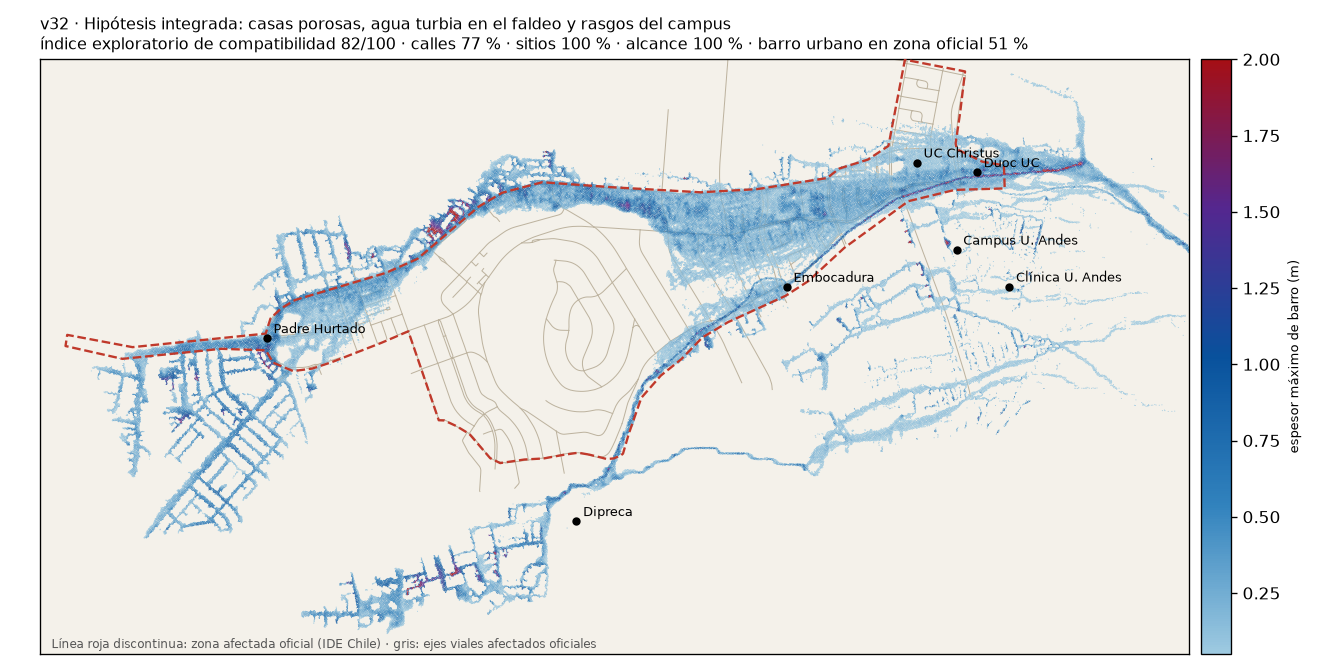
\includegraphics[width=\textwidth]{anexo/v32}\caption{Fact sheet v32: Integrated hypothesis: porous houses, turbid water on the lower hillside and campus features.}\end{figure}

\paragraph{z26 · Porous houses (fine time step).} \textbf{What it tests:} Allowing buildings in the official area to admit mud (floor at ground elevation plus 0.3 m and high resistance), instead of representing them as solid blocks. \textbf{What it shows:} Calculated: urban mud within the official area increases from 34 \% to 54 \%; it wets 36 \% of the official area and 40 \% of its affected properties; it meets the four original acceptance criteria. With half the resistance (v30), there is almost no change. \textbf{Model limitations:} The calculated depth next to the UC Christus emergency department drops to 0.30 m. The campus point remains dry with a fine time step. \textbf{What it raises:} In the model, assumed mud retention within lots modifies the calculated distribution within the official area; its representation remains an assumption. \textbf{Status:} ECI verified with a fine time step: 76/100 (subsequent fitting).

\begin{figure}[H]\centering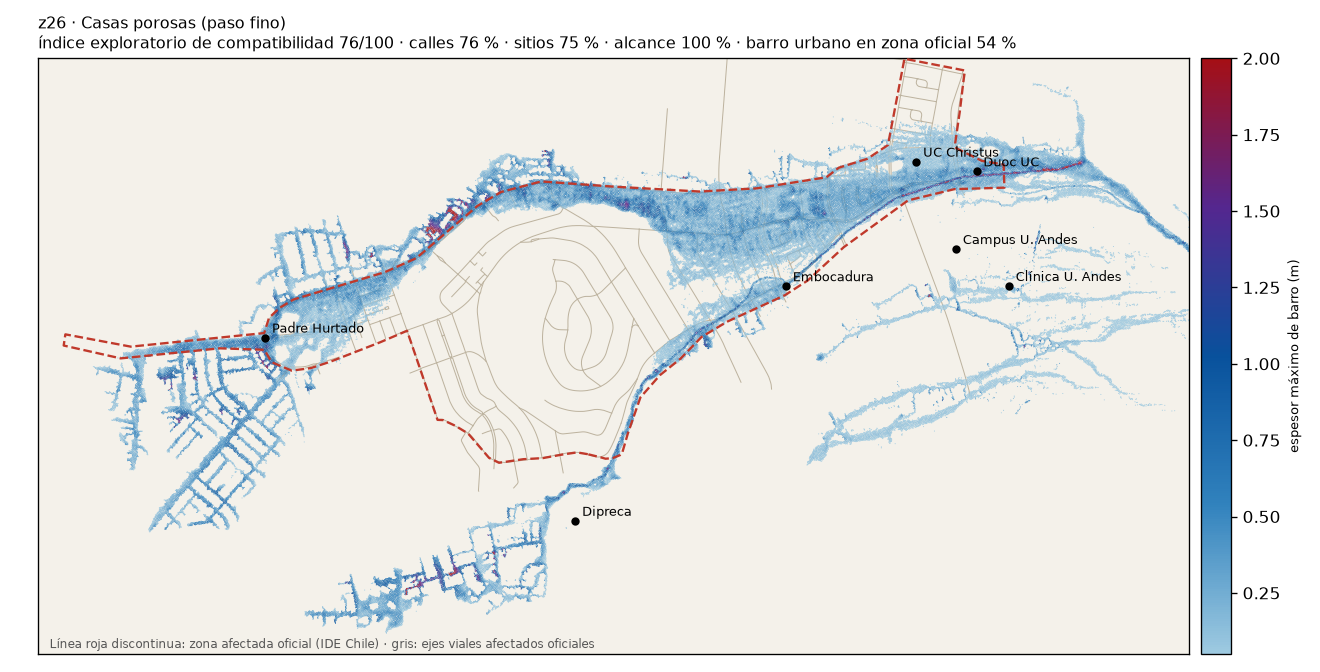
\includegraphics[width=\textwidth]{anexo/z26}\caption{Fact sheet z26: Porous houses (fine time step).}\end{figure}

\paragraph{z29 · More liquid fluid on the lower hillside (fine time step).} \textbf{What it tests:} Two mud mixtures depending on the area: Cv 0.27 on the lower hillside of the campus and Cv 0.43 in the main branch, with rainfall only outside the contributing catchments. \textbf{What it shows:} Calculated: the campus control point remains wet with a fine time step (0.09 m), unlike the hypothesis with a single mud mixture (0.01 m). \textbf{Model limitations:} It does not reduce mud outside the official area: the fraction within it remains at 0.35. \textbf{What it raises:} In these tests, an assumed more liquid fluid on the lower hillside, compatible with the turbid water interpreted in the Meganoticias video, also produces flow on campus with a fine time step. \textbf{Status:} ECI verified with a fine time step: 78/100 (subsequent fitting).

\begin{figure}[H]\centering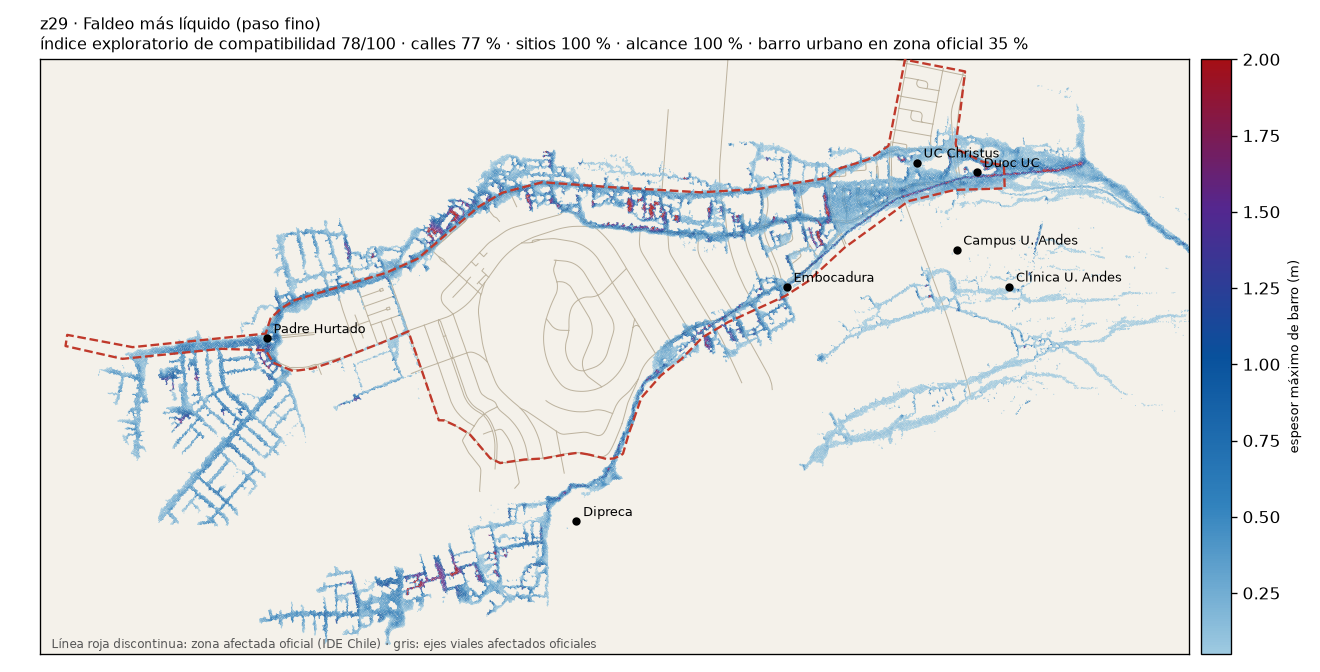
\includegraphics[width=\textwidth]{anexo/z29}\caption{Fact sheet z29: More liquid fluid on the lower hillside (fine time step).}\end{figure}

\subsection*{Hypothesis selected for the held-out test}

\paragraph{z02 · Channel + southern branches + hillside rainfall, full city (fine time step).} \textbf{What it tests:} The hypothesis selected before the test with held-out observations: mud emerges through the main channel onto the alluvial fan and through the southern branches, with rainfall of 35 mm/h also applied over the burned hillside. It repeats v02 with a time step four times finer to examine sensitivity to the time step. \textbf{What it shows:} Calculated: simulated flow follows the two corridors delimiting the official area (El Alba–General Blanche and Quebrada Honda) and comes within 200 m of Padre Hurtado; around Clínica UC Christus it calculates 1.13 m (Cadena 3 reported about 1 m in the emergency department) and produces flow next to Clínica U. de los Andes. The indicators match those of v02; this numerical check does not validate the event reconstruction. \textbf{Model limitations:} Only one third of simulated mud in urban areas falls within the official area: it extends west of Padre Hurtado, along Quebrada Honda towards Dipreca and, because of the applied rainfall, along streets in other neighborhoods. It does not reach the U. de los Andes campus. Part of the applied rainfall (about 9,400 m$^3$) overlaps catchments already entering through the hydrographs; v28 corrects this. \textbf{What it raises:} In z02, hillside rainfall contributes to reproducing flow next to the clinic; the result does not establish its contribution during the event. Building representation, coarse load and vegetation are considered possible explanations for the extent outside the official area (v25–v27). \textbf{Status:} Hypothesis selected before the test with held-out observations (unfavorable test result): ECI 72/100. Subsequent tests (porous houses, liquid fluid on the lower hillside, integrated hypothesis) outperform it through fitting.

\begin{figure}[H]\centering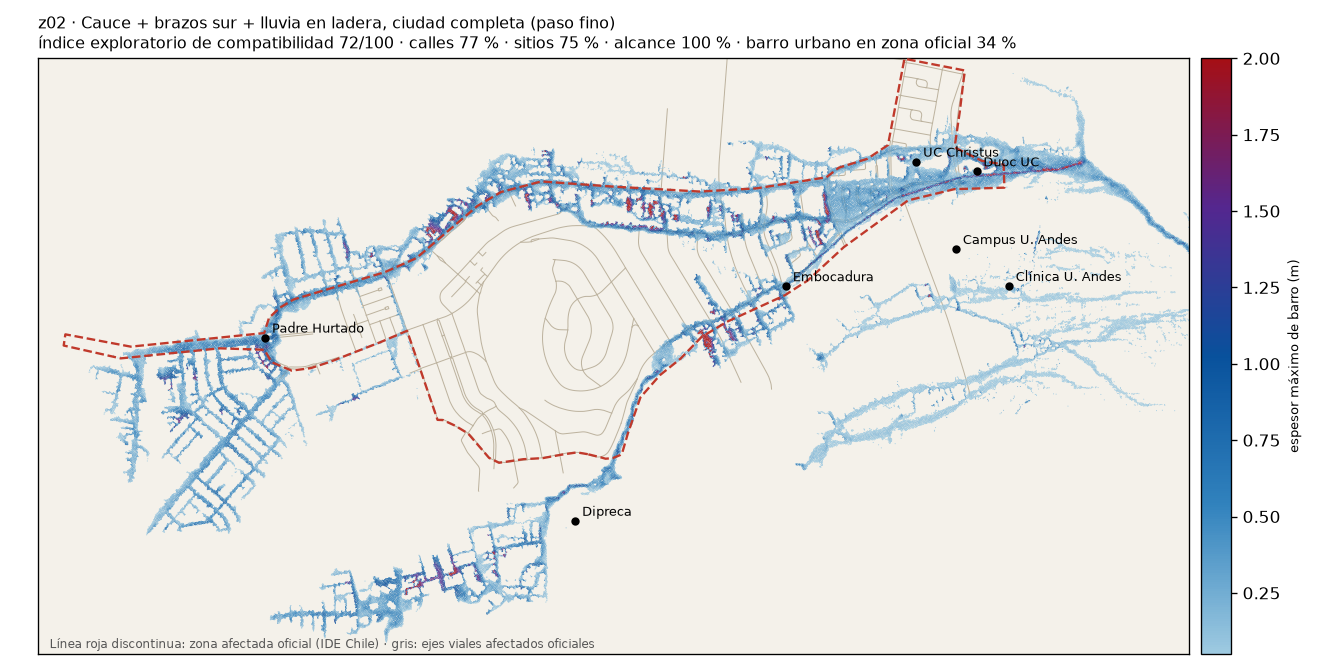
\includegraphics[width=\textwidth]{anexo/z02}\caption{Fact sheet z02: Channel + southern branches + hillside rainfall, full city (fine time step).}\end{figure}

\subsection*{Full city}

\paragraph{v01 · Main channel only, culvert with assumed zero capacity (300 thousand m$^3$).} \textbf{What it tests:} All mud emerges through the main channel onto the alluvial fan, with the General Blanche conduits and the Bulnes Correa culvert assumed to have zero capacity (hypothetical scenario). \textbf{What it shows:} Calculated: with the 42 thousand buildings, flow is channeled along streets; it calculates 1.16 m around UC Christus (0.3 m with the previous terrain), 1.9 m next to Duoc UC, comes within 96 m of Padre Hurtado and wets Quebrada Honda. \textbf{Model limitations:} It does not reproduce impacts next to Clínica U. de los Andes, on La Plaza Sur or on the campus. \textbf{What it raises:} This configuration does not reproduce impacts in the southern sector. Inflows from that sector are one of the hypotheses considered to explain the discrepancy. \textbf{Status:} Reference: ECI 68/100.

\begin{figure}[H]\centering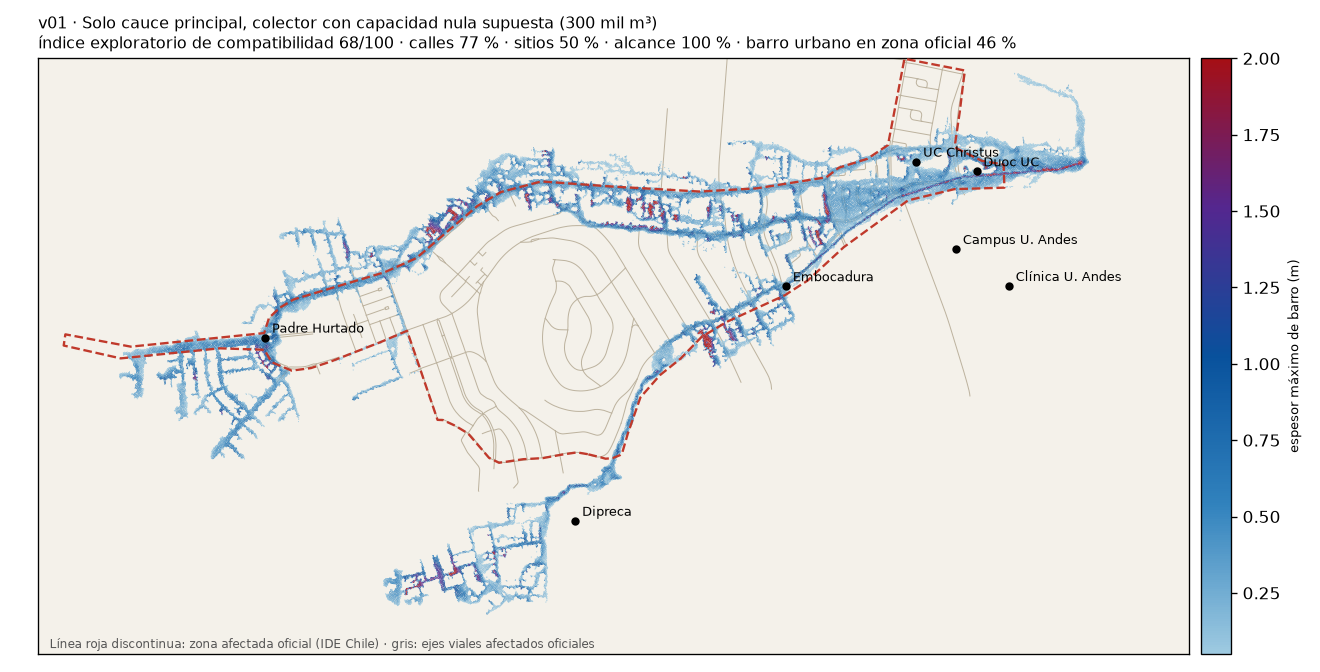
\includegraphics[width=\textwidth]{anexo/v01}\caption{Fact sheet v01: Main channel only, culvert with assumed zero capacity (300 thousand m$^3$).}\end{figure}

\paragraph{v07 · Main channel only with 150 thousand m$^3$.} \textbf{What it tests:} Same as v01, but with half the volume: the central value of the first rainfall-based estimate. \textbf{What it shows:} Calculated: the front stops 348 m from Padre Hurtado. \textbf{Model limitations:} It does not meet the reach criterion. \textbf{What it raises:} In the scenarios tested and under their assumptions, about 300 thousand m$^3$ allows the reach criterion to be reproduced; that order of magnitude is consistent with a rainfall-based estimate adopting the soil saturation reported by the authority. \textbf{Status:} The low-volume configuration does not meet the reach criterion: ECI 67/100.

\begin{figure}[H]\centering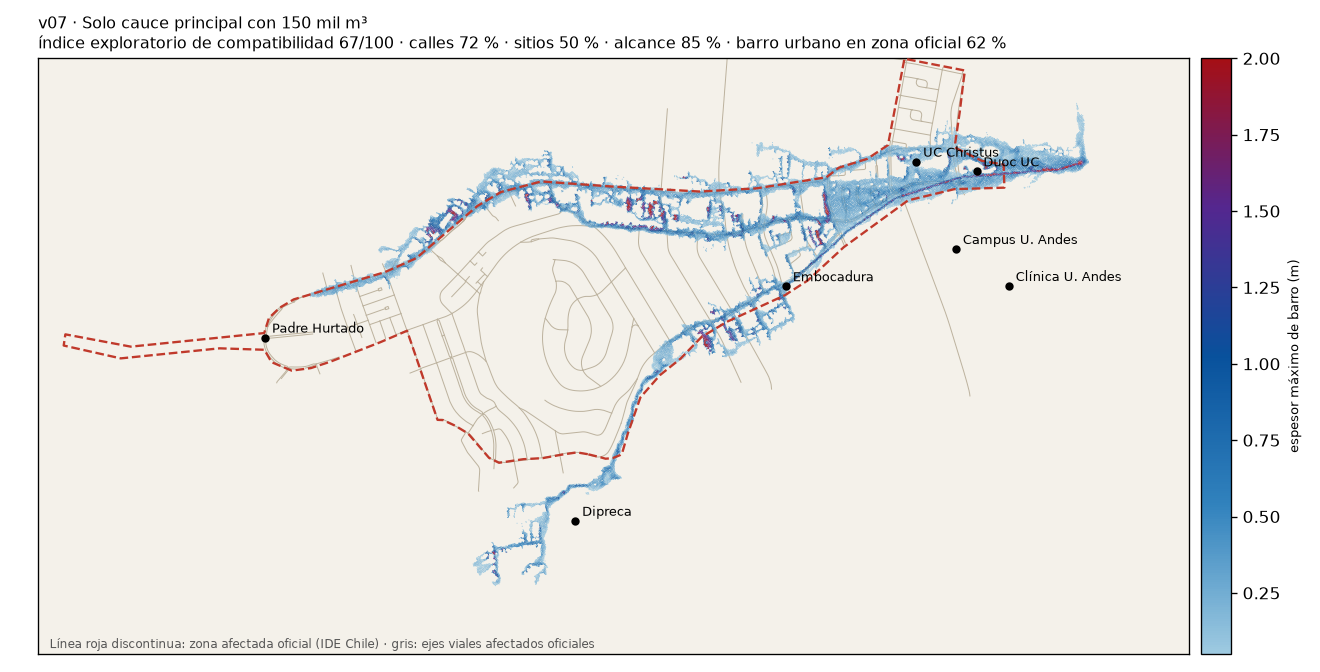
\includegraphics[width=\textwidth]{anexo/v07}\caption{Fact sheet v07: Main channel only with 150 thousand m$^3$.}\end{figure}

\subsection*{U. Andes campus}

\paragraph{v21 · Southern branch along the official channel, without hillside rainfall.} \textbf{What it tests:} The southern branch follows the official hydrographic network alignment to upper Av. Álvaro del Portillo, where the official alignment ends and the model allows flow to discharge onto the avenue. Without hillside rainfall, to isolate its effect. \textbf{What it shows:} Calculated: mud from the southern branch reaches the avenue (0.48 m where the channel ends) and runs down it towards La Plaza and General Blanche, in a manner compatible with what Cooperativa attributed to the vice-rector and La Tercera to Carabineros. \textbf{Model limitations:} Without hillside rainfall, the impact next to Clínica U. de los Andes is not reproduced (0 m) and flow does not reach the Biblioteca. \textbf{What it raises:} In the configurations compared, hillside rainfall allows impacts next to the clinic to be reproduced, and, in the model, the southern branch generates an overflow compatible with the one the vice-rector described to Cooperativa on the north side of the campus. \textbf{Status:} ECI 68/100.

\begin{figure}[H]\centering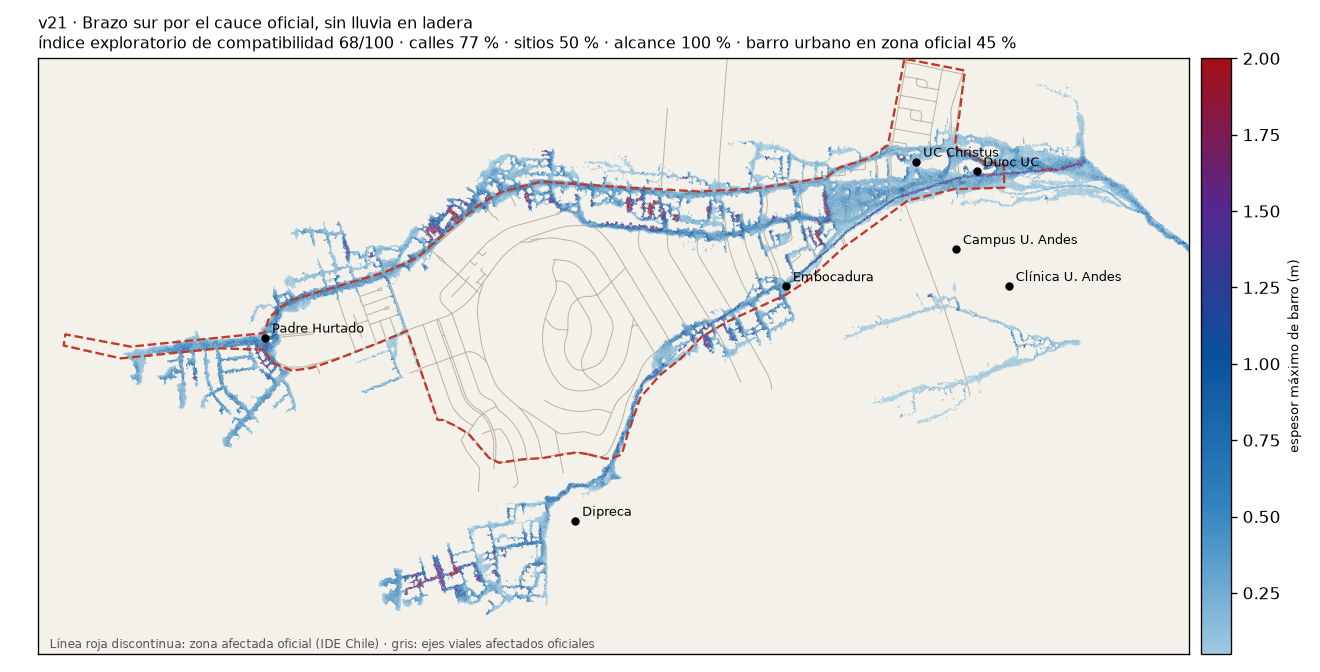
\includegraphics[width=\textwidth]{anexo/v21}\caption{Fact sheet v21: Southern branch along the official channel, without hillside rainfall.}\end{figure}

\paragraph{v19 · Southern branch along the official channel to Álvaro del Portillo + rainfall (fine time step).} \textbf{What it tests:} The selected hypothesis (z02) with the southern branch traced according to official mapping, to examine whether flow reaches the campus and the Aula Magna. \textbf{What it shows:} Calculated: it reproduces an overflow in upper Álvaro del Portillo and its descent along the avenue, in addition to what z02 achieves. \textbf{Model limitations:} Simulated flow continues along the avenue, which is steeper ($\sim$8 \%) than the woodland towards the Biblioteca ($\sim$4 \%), and does not reach the depression next to the building or the campus control point (1 cm). \textbf{What it raises:} In subsequent microsimulations, the assumed overflow does not reach the courtyard with any of the fluids tested; the most compatible scenario assumes turbid hillside runoff that, in the model, follows La Plaza Sur and enters through a clearing, with carved features unresolved by the 30 m terrain. \textbf{Status:} ECI 71/100. Superseded as a fit by the scenario with assumed local runoff input (see v32); the actual origin of the water is not determined.

\begin{figure}[H]\centering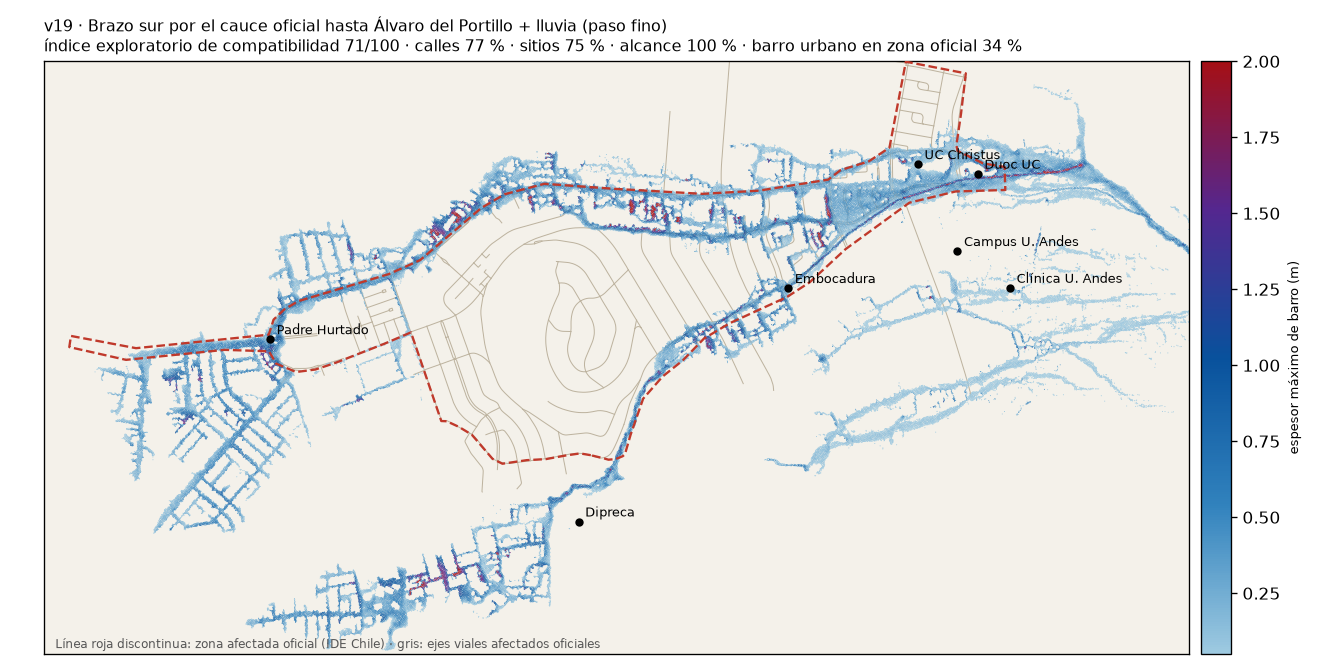
\includegraphics[width=\textwidth]{anexo/v19}\caption{Fact sheet v19: Southern branch along the official channel to Álvaro del Portillo + rainfall (fine time step).}\end{figure}

\subsection*{Bulnes Correa culvert (hypothetical scenarios)}

\paragraph{v17 · Hypothetical scenario: assumed culvert capacity set to 30 m$^3$/s.} \textbf{What it tests:} Hypothetical scenario with assumed culvert capacity set to 30 m$^3$/s and capture of the entire channel cross section. Public information on the actual capacity and condition of the culvert was unavailable. \textbf{What it shows:} Calculated: the modeled culvert reaches the imposed capacity (removes 67.6 thousand m$^3$ at 30 m$^3$/s) and Quebrada Honda is wetted at 62 \% of its points. \textbf{Model limitations:} — \textbf{What it raises:} In the model, with an assumed capacity of 30 m$^3$/s, surface flow remains towards Quebrada Honda. This is not an evaluation of the real structure. \textbf{Status:} Lower reference for the interval explored in these scenarios: ECI 69/100.

\begin{figure}[H]\centering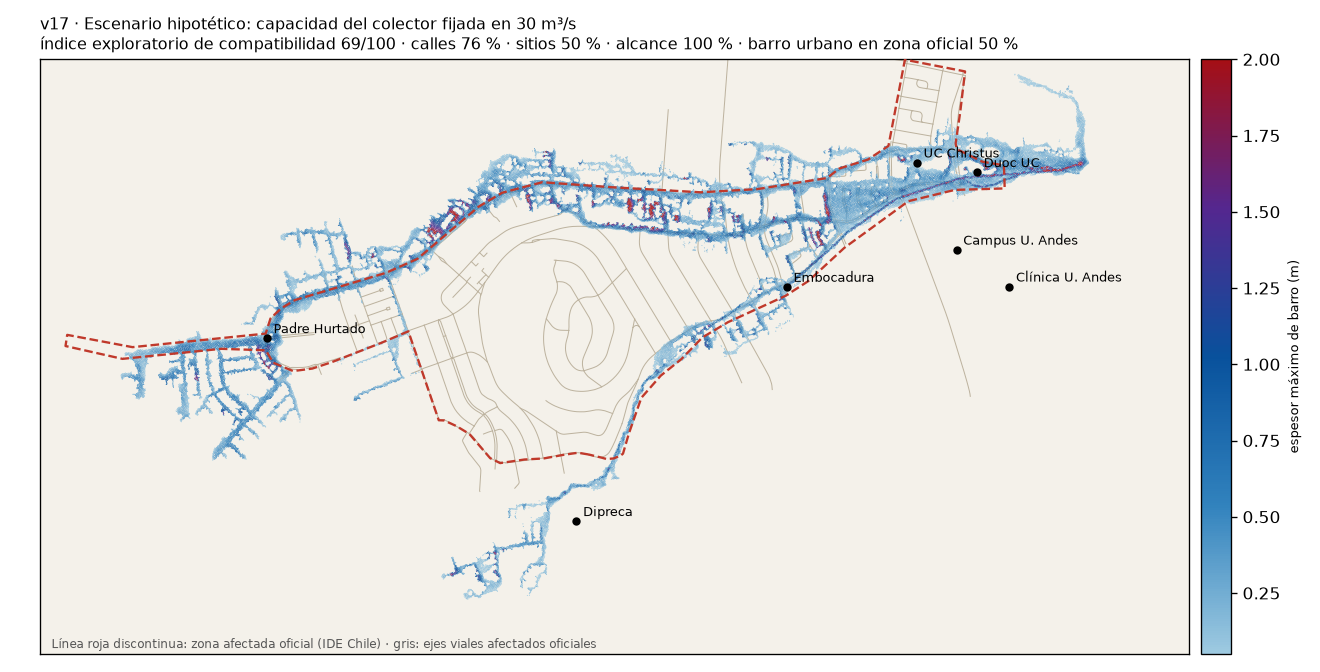
\includegraphics[width=\textwidth]{anexo/v17}\caption{Fact sheet v17: Hypothetical scenario: assumed culvert capacity set to 30 m$^3$/s.}\end{figure}

\paragraph{v10 · Hypothetical scenario: assumed culvert capacity set to 100 m$^3$/s.} \textbf{What it tests:} Hypothetical high-capacity scenario with capture of the entire channel cross section. \textbf{What it shows:} Calculated: the modeled culvert removes about 93 thousand m$^3$ with a peak of $\sim$64 m$^3$/s and Quebrada Honda remains dry. With 200 m$^3$/s the result is the same, because calculated arriving discharge does not exceed $\sim$65 m$^3$/s. \textbf{Model limitations:} The scenario does not reproduce the reported flooding of Quebrada Honda; this discrepancy does not allow the operation of the real culvert to be established. \textbf{What it raises:} Under the assumptions tested and with full capture, the analysis places the calculated threshold of assumed capacity for removing all surface flow in the model near 65 m$^3$/s. A capture radius of 12 m allowed flow to pass beside the sink: this was a representation artifact, now corrected. \textbf{Status:} Upper reference for the interval explored in these scenarios: ECI 68/100.

\begin{figure}[H]\centering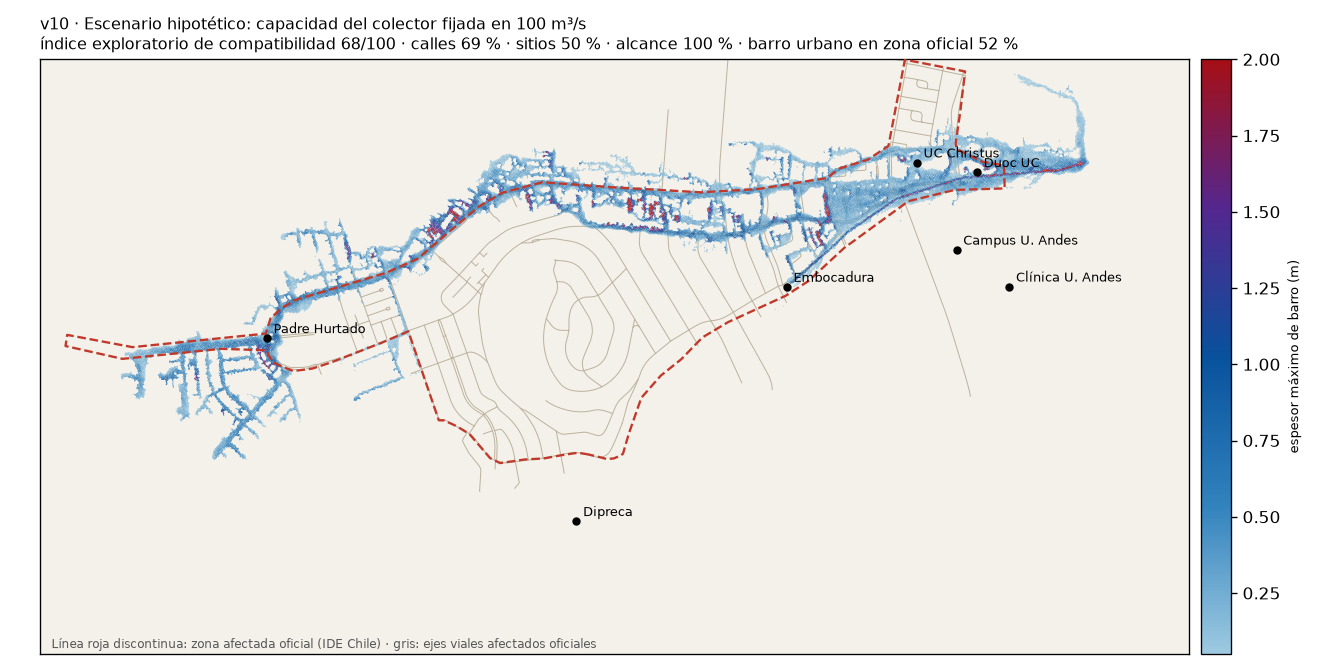
\includegraphics[width=\textwidth]{anexo/v10}\caption{Fact sheet v10: Hypothetical scenario: assumed culvert capacity set to 100 m$^3$/s.}\end{figure}

\subsection*{Mud type}

\paragraph{v08 · Thick mud (Glenwood 1, Cv 0.45).} \textbf{What it tests:} A more concentrated and viscous mud mixture (1,742 kg/m$^3$, yield stress 29 Pa). \textbf{What it shows:} Calculated: the front stops 396 m from Padre Hurtado. \textbf{Model limitations:} It does not meet the reach criterion. \textbf{What it raises:} An intermediate material (Cv 0.43, v25) does not reduce mud outside the official area; across the full Cv range from 0.24 to 0.48 (concentration quadrature), the index remains between 71 and 73. \textbf{Status:} Thicker variant: ECI 67/100.

\begin{figure}[H]\centering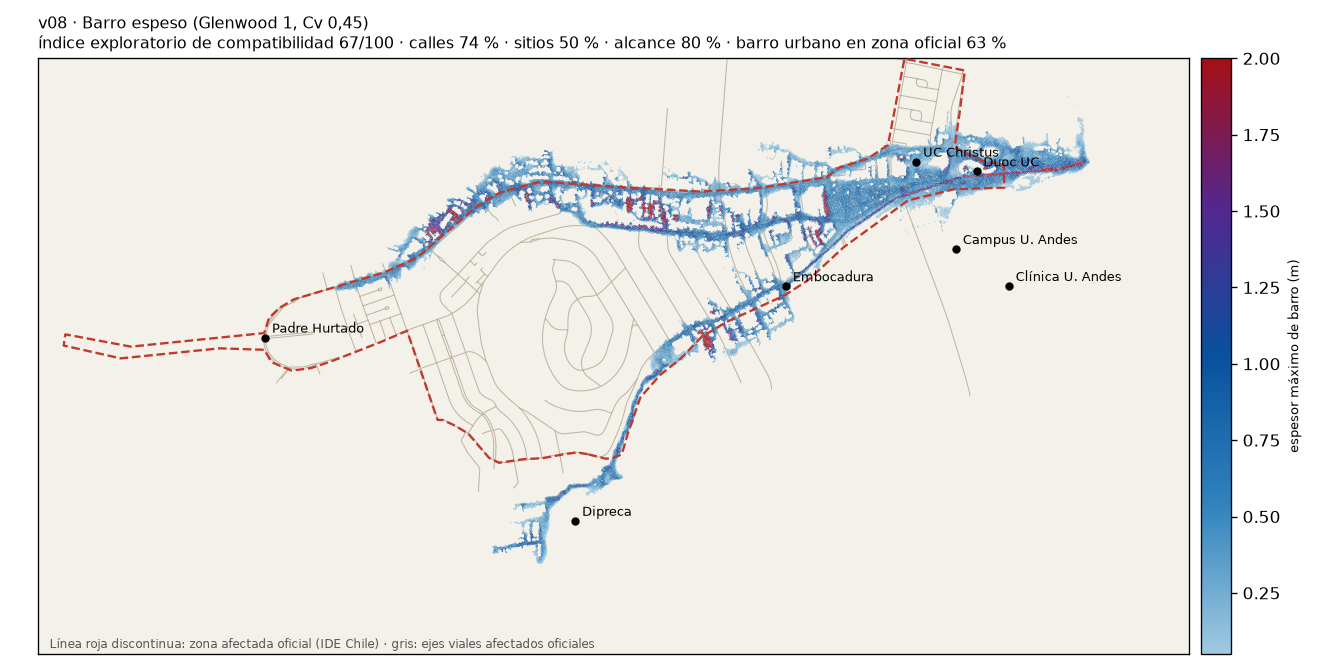
\includegraphics[width=\textwidth]{anexo/v08}\caption{Fact sheet v08: Thick mud (Glenwood 1, Cv 0.45).}\end{figure}

\paragraph{v09 · Very fluid mud (Aspen 2).} \textbf{What it tests:} A more fluid mud mixture than the reference. \textbf{What it shows:} Calculated: a result similar to the reference (ECI 70/100), with somewhat more mud inside the official area. \textbf{Model limitations:} It does not reach the southern sector (without southern branches or rainfall). \textbf{What it raises:} The ECI varies little between the materials tested; that variation alone does not summarize changes in reach, depth or velocity. \textbf{Status:} Index sensitivity to material: low. ECI 70/100.

\begin{figure}[H]\centering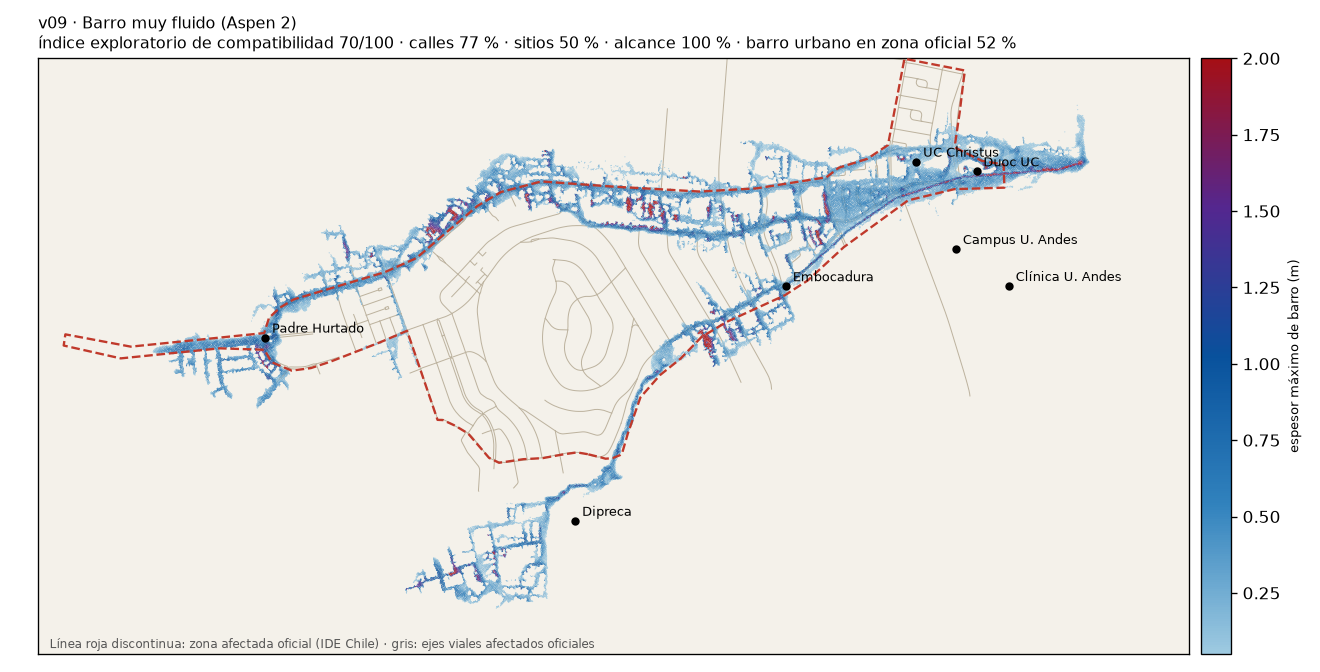
\includegraphics[width=\textwidth]{anexo/v09}\caption{Fact sheet v09: Very fluid mud (Aspen 2).}\end{figure}

\subsection*{Previous terrain (first model generation)}

\paragraph{e04 · Channel + culvert with assumed zero capacity, terrain with 1,103 buildings.} \textbf{What it tests:} The configuration selected in the first model generation (9 October), with only 1,103 buildings represented and the press-perimeter criterion. \textbf{What it shows:} Calculated: flow spreads more across the surface (93 ha inside the official area) in thinner layers and reaches Padre Hurtado. \textbf{Model limitations:} It calculates only 0.3 m around UC Christus (Cadena 3 reported about 1 m in the emergency department). \textbf{What it raises:} Representing all buildings changed the results; representation as impermeable blocks could intensify channeling compared with one that allows retention in buildings (v26). \textbf{Status:} Superseded by simulations with the full city: ECI 68/100.

\begin{figure}[H]\centering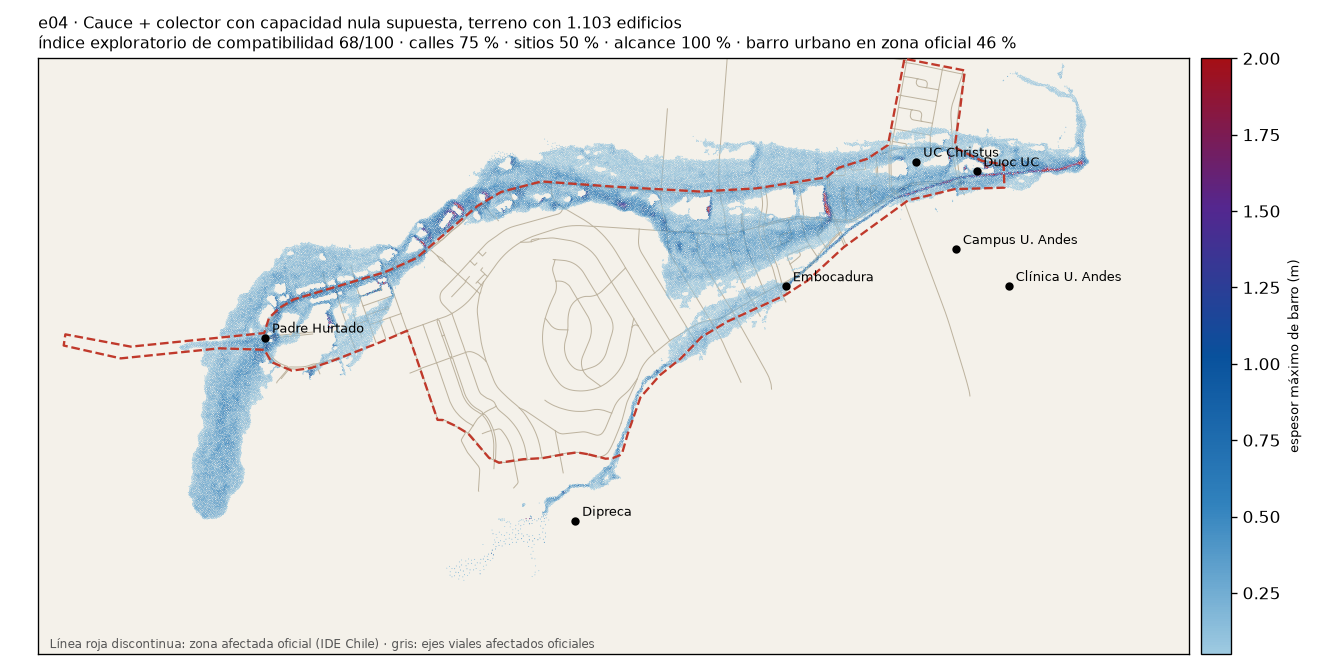
\includegraphics[width=\textwidth]{anexo/e04}\caption{Fact sheet e04: Channel + culvert with assumed zero capacity, terrain with 1,103 buildings.}\end{figure}

\paragraph{f03 · Alluvial fan + culvert inlet + hillside rainfall, previous terrain.} \textbf{What it tests:} The first simulation with hillside rainfall, using the previous terrain. \textbf{What it shows:} Calculated: it was the first to produce flow next to Clínica U. de los Andes and on La Plaza Sur. \textbf{Model limitations:} Low thickness around UC Christus and extent outside the official area. \textbf{What it raises:} It led to the hypothesis selected for the held-out test (channel + southern branches + rainfall, z02). \textbf{Status:} ECI 71/100.

\begin{figure}[H]\centering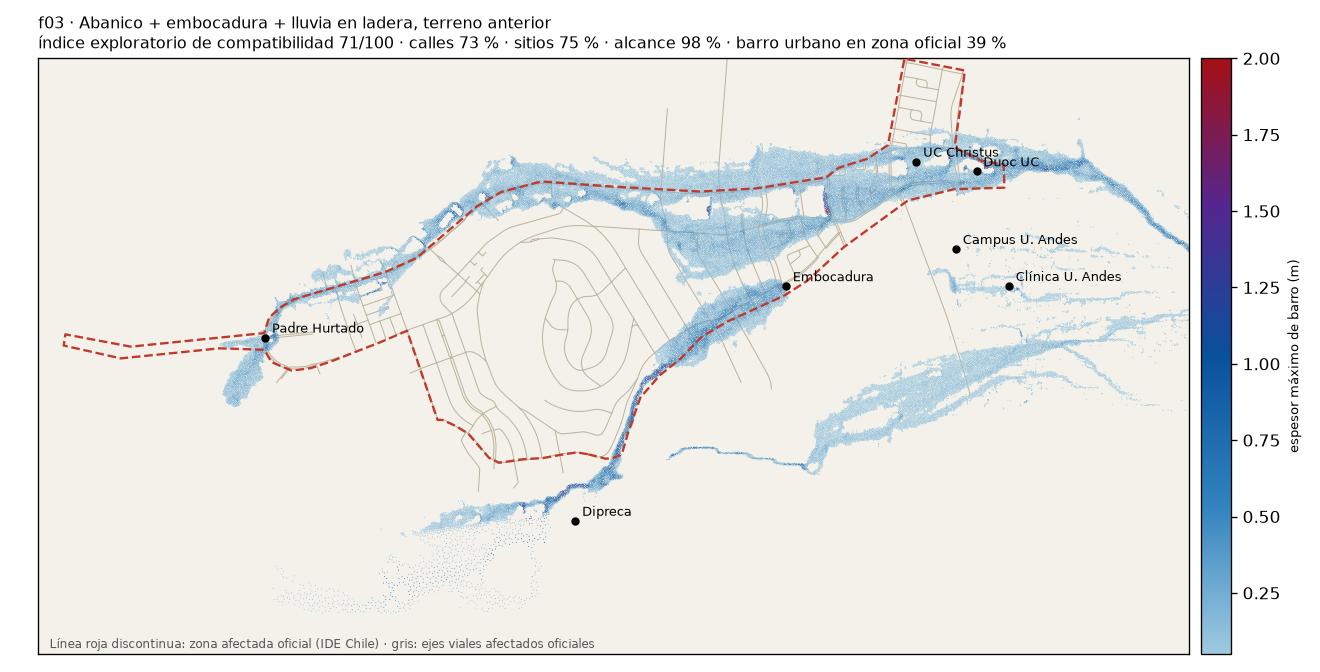
\includegraphics[width=\textwidth]{anexo/f03}\caption{Fact sheet f03: Alluvial fan + culvert inlet + hillside rainfall, previous terrain.}\end{figure}

\paragraph{e03 · Overflow at the culvert inlet only (H2).} \textbf{What it tests:} Surface inflow of the entire assumed volume at Francisco Bulnes Correa, without inferring the actual operation of the channel. \textbf{What it shows:} Calculated: it wets Quebrada Honda but none of the alluvial fan. \textbf{Model limitations:} It does not reproduce General Blanche, Camino El Alba, Duoc UC or UC Christus. \textbf{What it raises:} El Desconcierto reports an overflow at Bulnes Correa described by Carabineros. Simulation e03 alone does not reproduce the full set of observations. \textbf{Status:} Does not by itself reproduce the full set of observations under the assumptions and terrain of e03: ECI 16/100.

\begin{figure}[H]\centering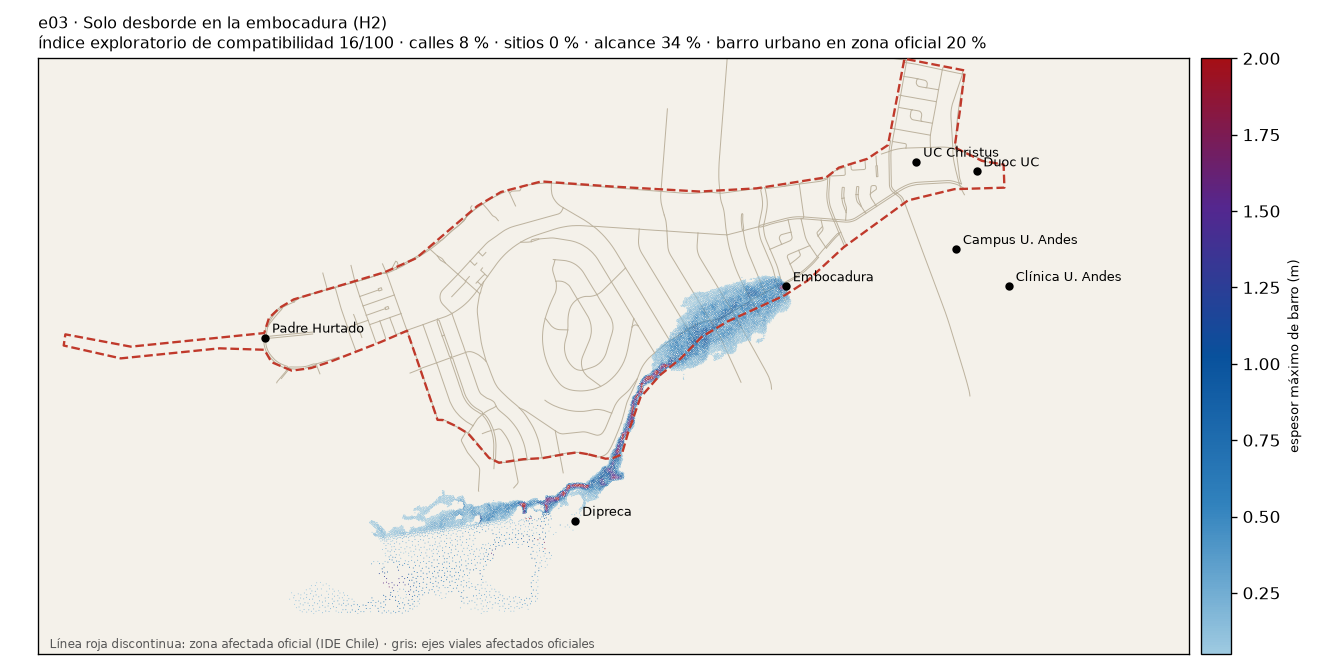
\includegraphics[width=\textwidth]{anexo/e03}\caption{Fact sheet e03: Overflow at the culvert inlet only (H2).}\end{figure}

\end{document}
